\chapter{Desarrollo}
\label{hardware}

\section{Búsqueda de información}
\label{busqueda_informacion}

El primer paso es identificar el hardware del que disponemo en la fábrica con ayuda de las fotos tomadas:
    \begin{figure}[H]
            \centering
            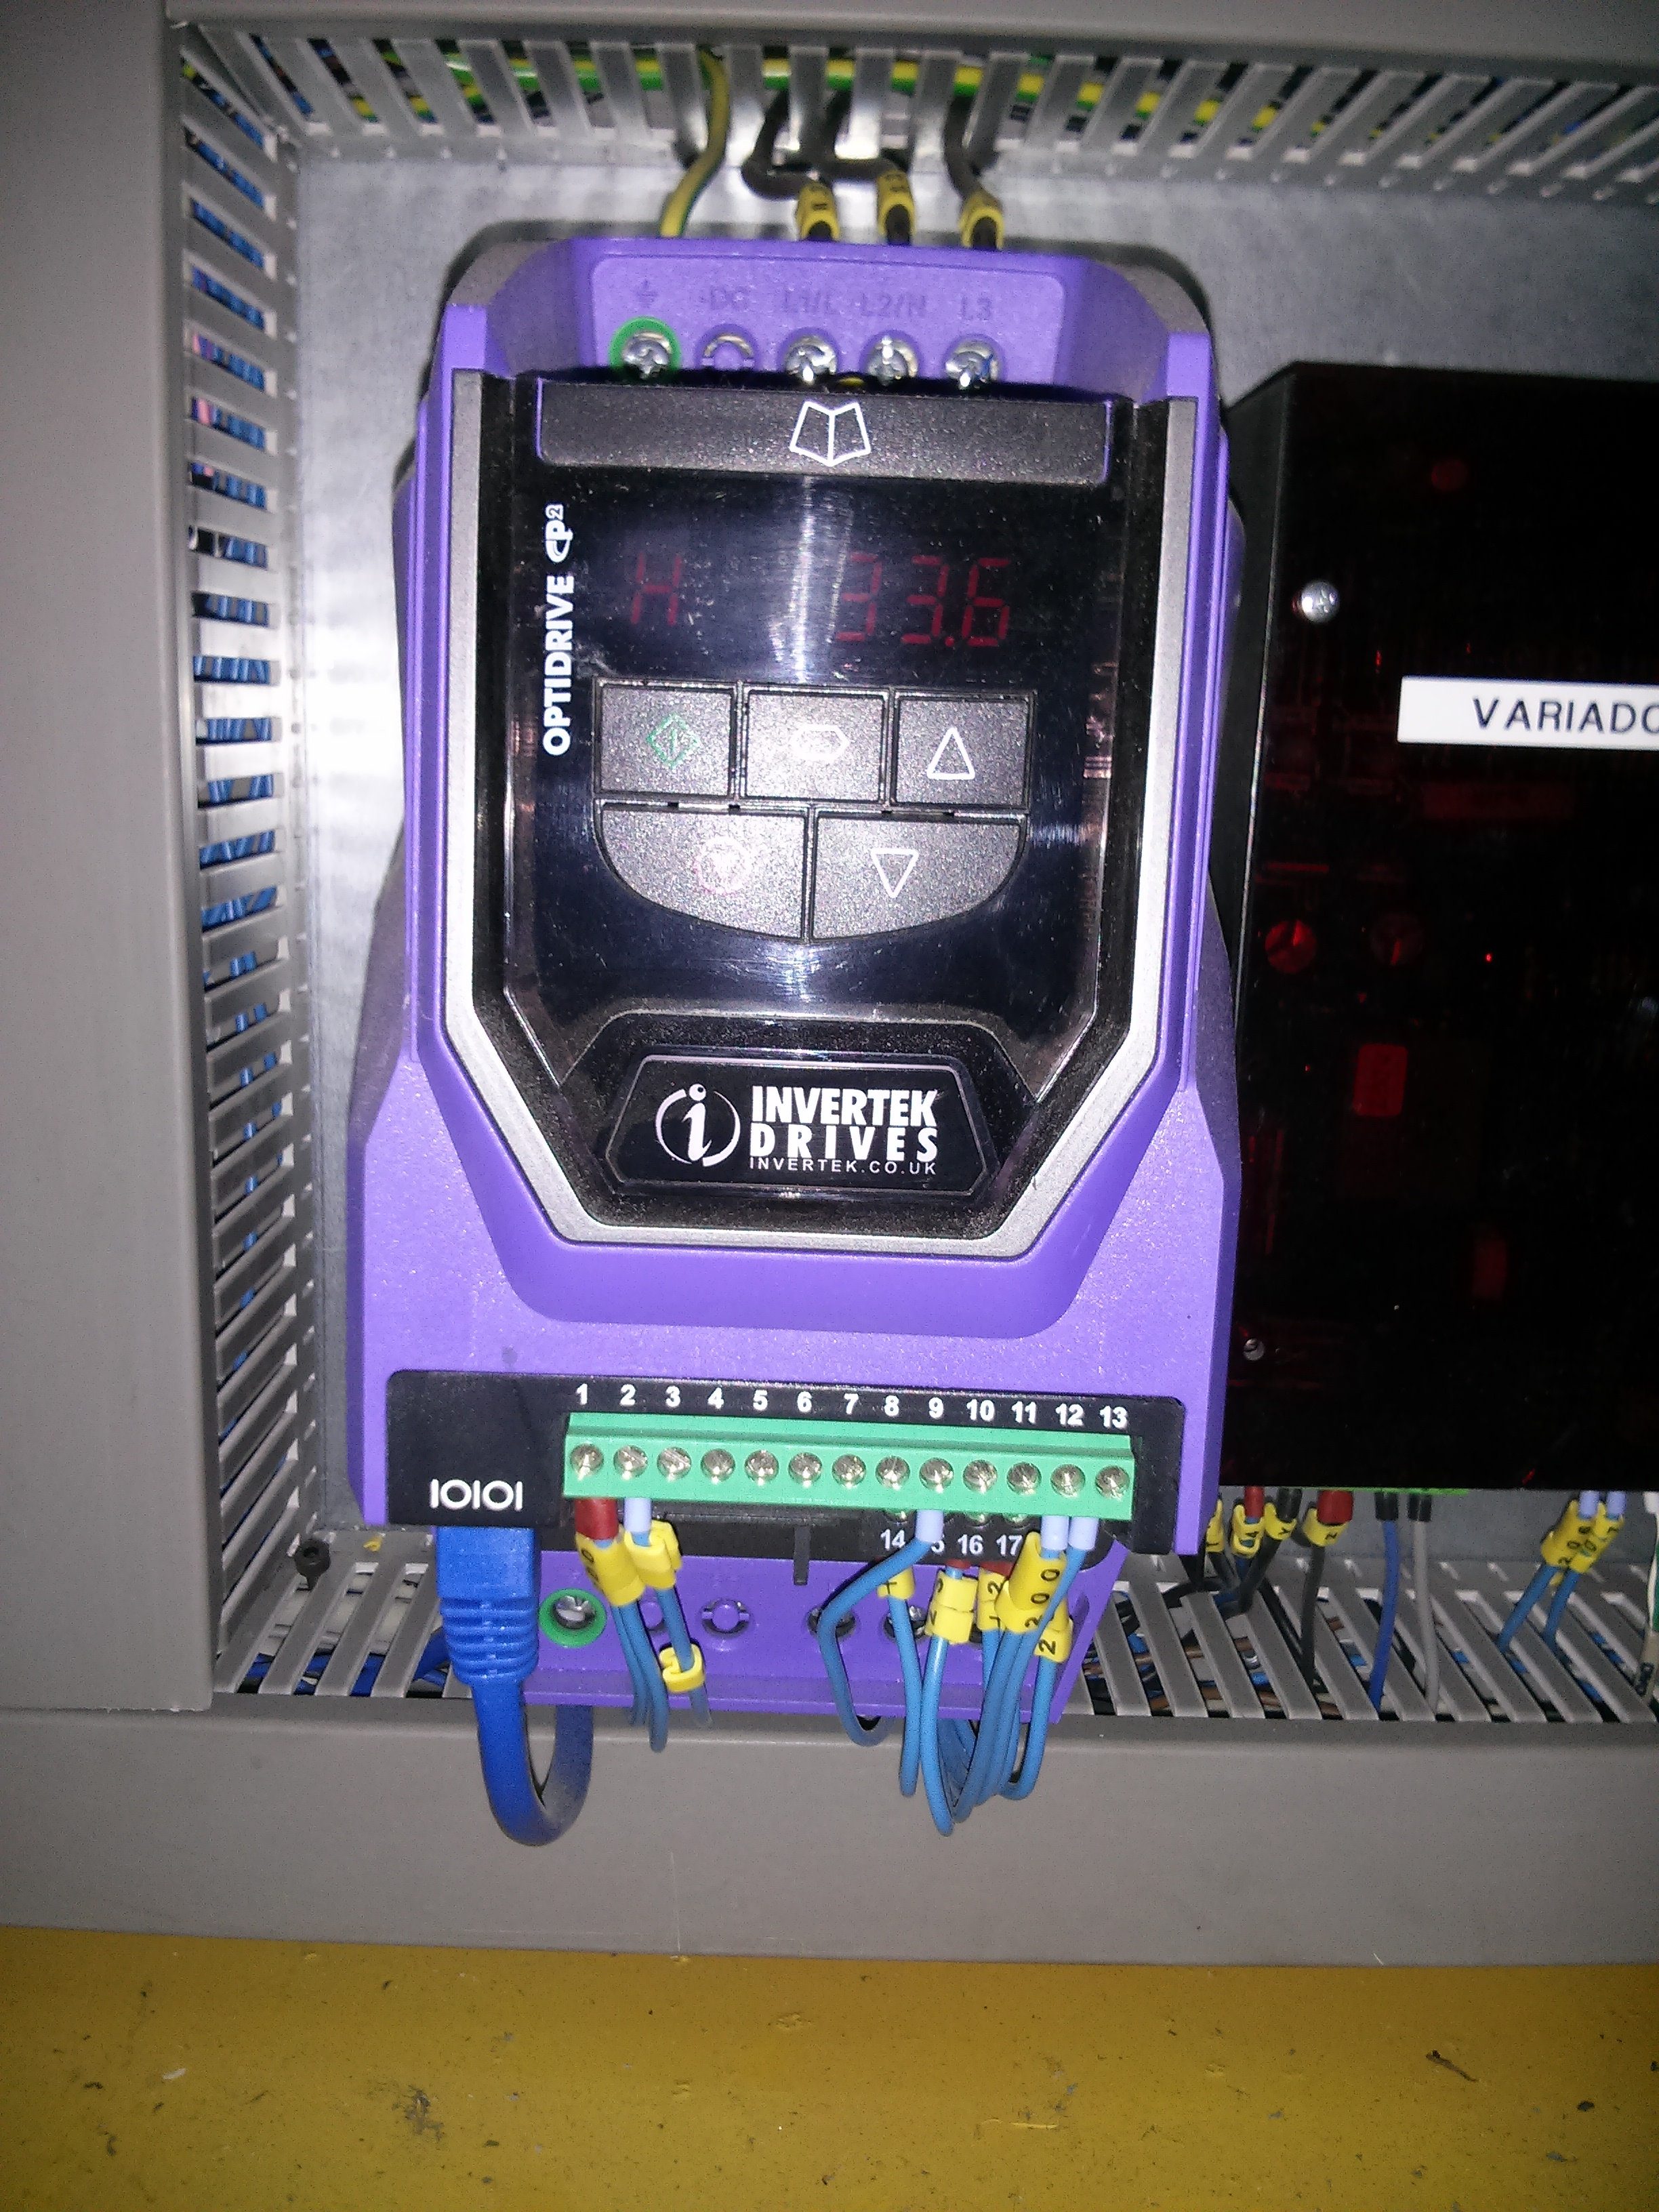
\includegraphics[width=0.4\textwidth]{images/huesca/IMG_20141216_174810.jpg}
            \caption{Variador Optidrive}
            \label{fig:hardware_variador}
    \end{figure}

    \begin{figure}[H]
            \centering
            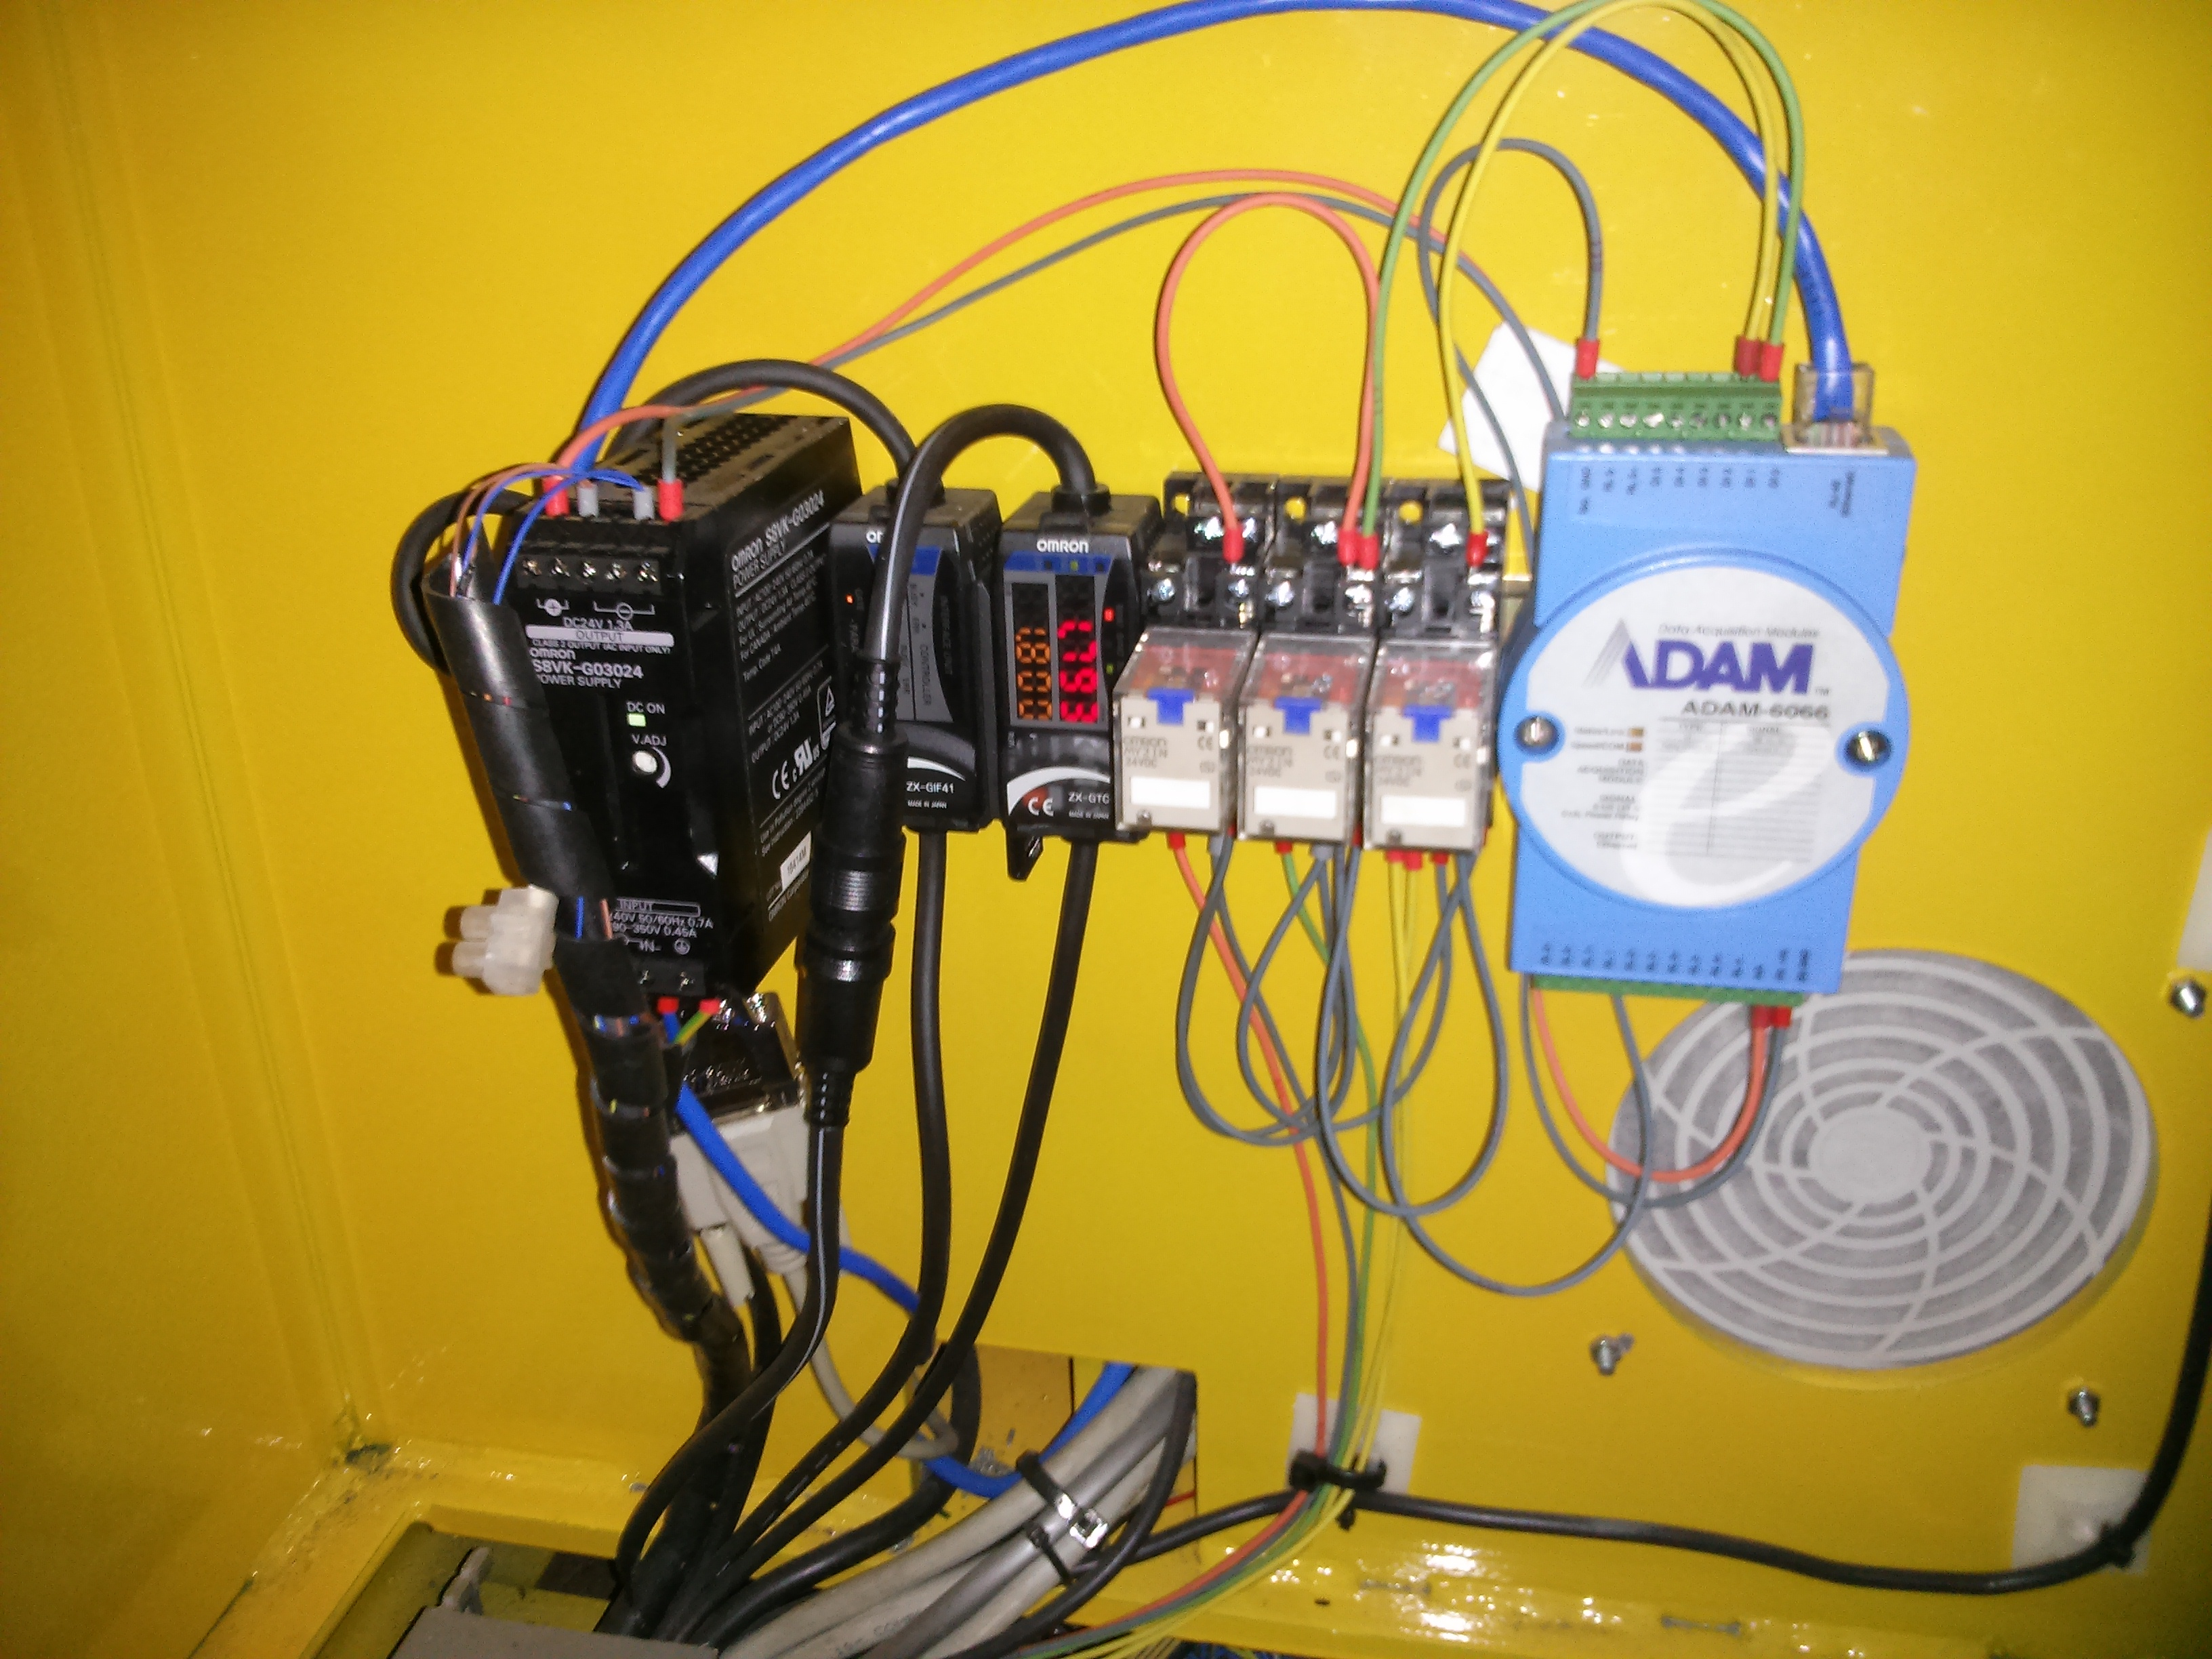
\includegraphics[width=0.4\textwidth]{images/huesca/IMG_20141216_174824.jpg}
            \caption{Sensor de diámetro y perifería}
            \label{fig:hardware_diametro}
    \end{figure}

    \begin{figure}[H]
            \centering
            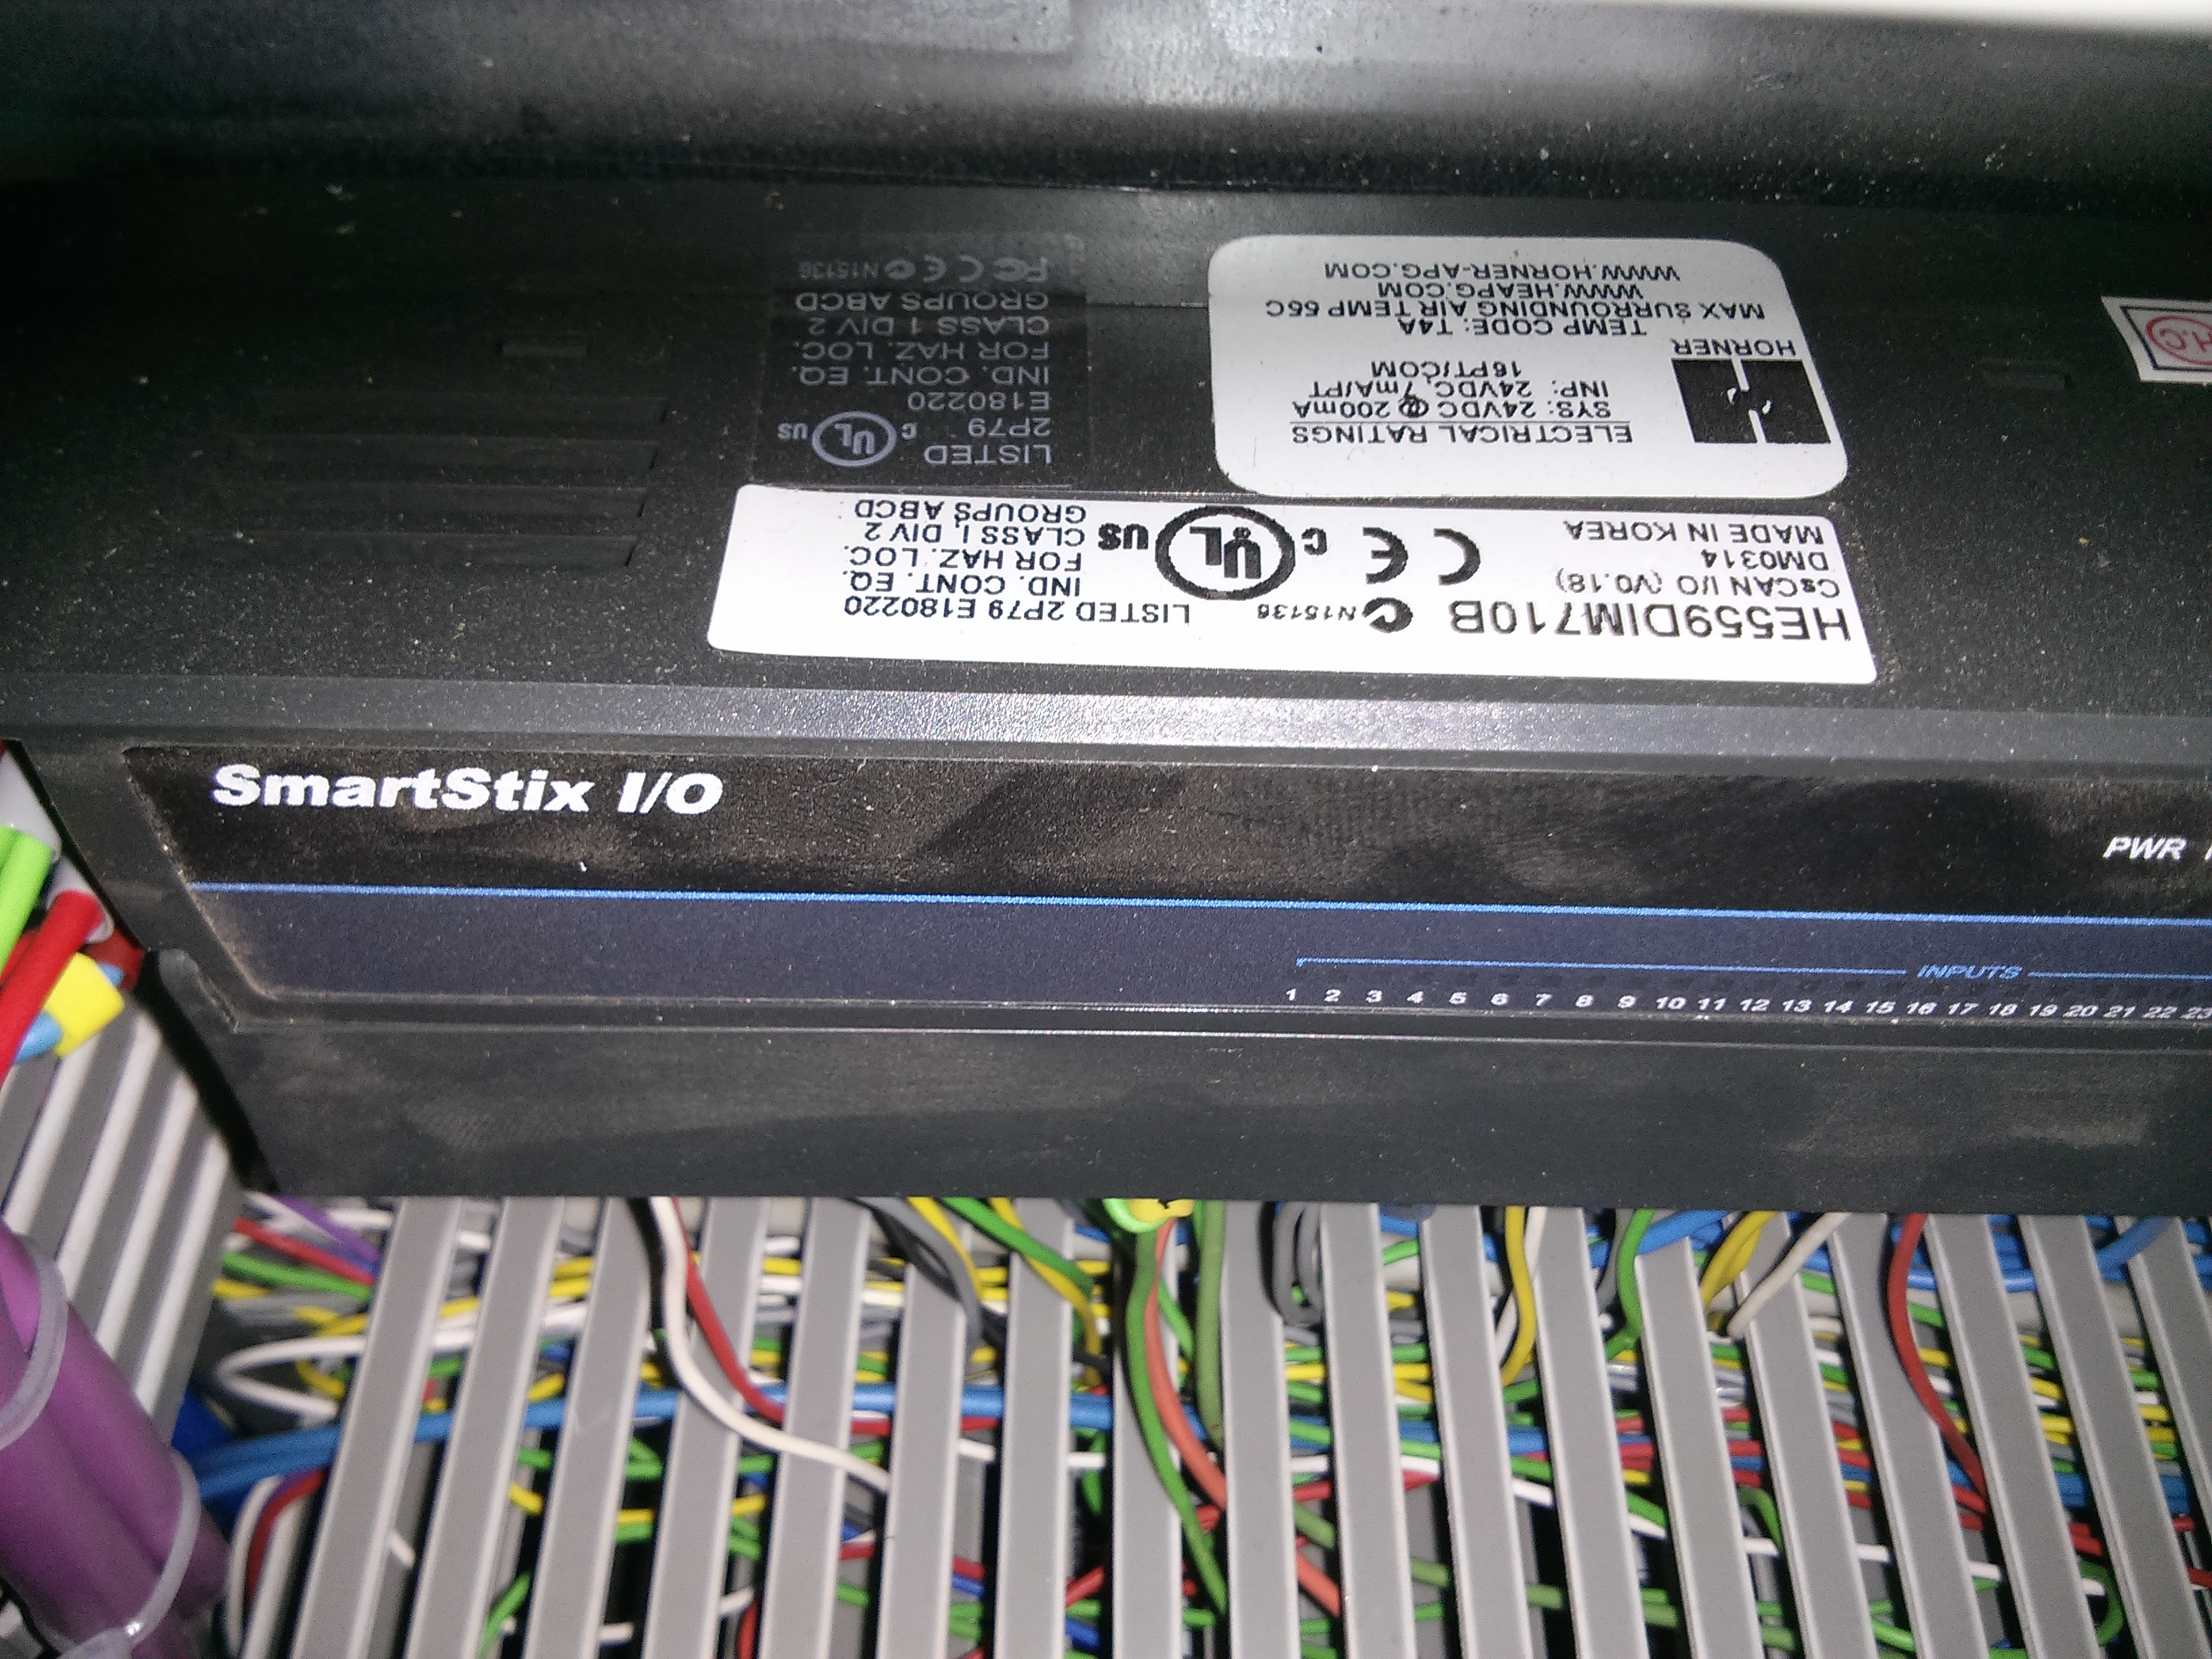
\includegraphics[width=0.4\textwidth]{images/huesca/IMG_20141216_174925.jpg}
            \caption{Perifería distribuida}
            \label{fig:hardware_periferia}
    \end{figure}

    \begin{figure}[H]
            \centering
            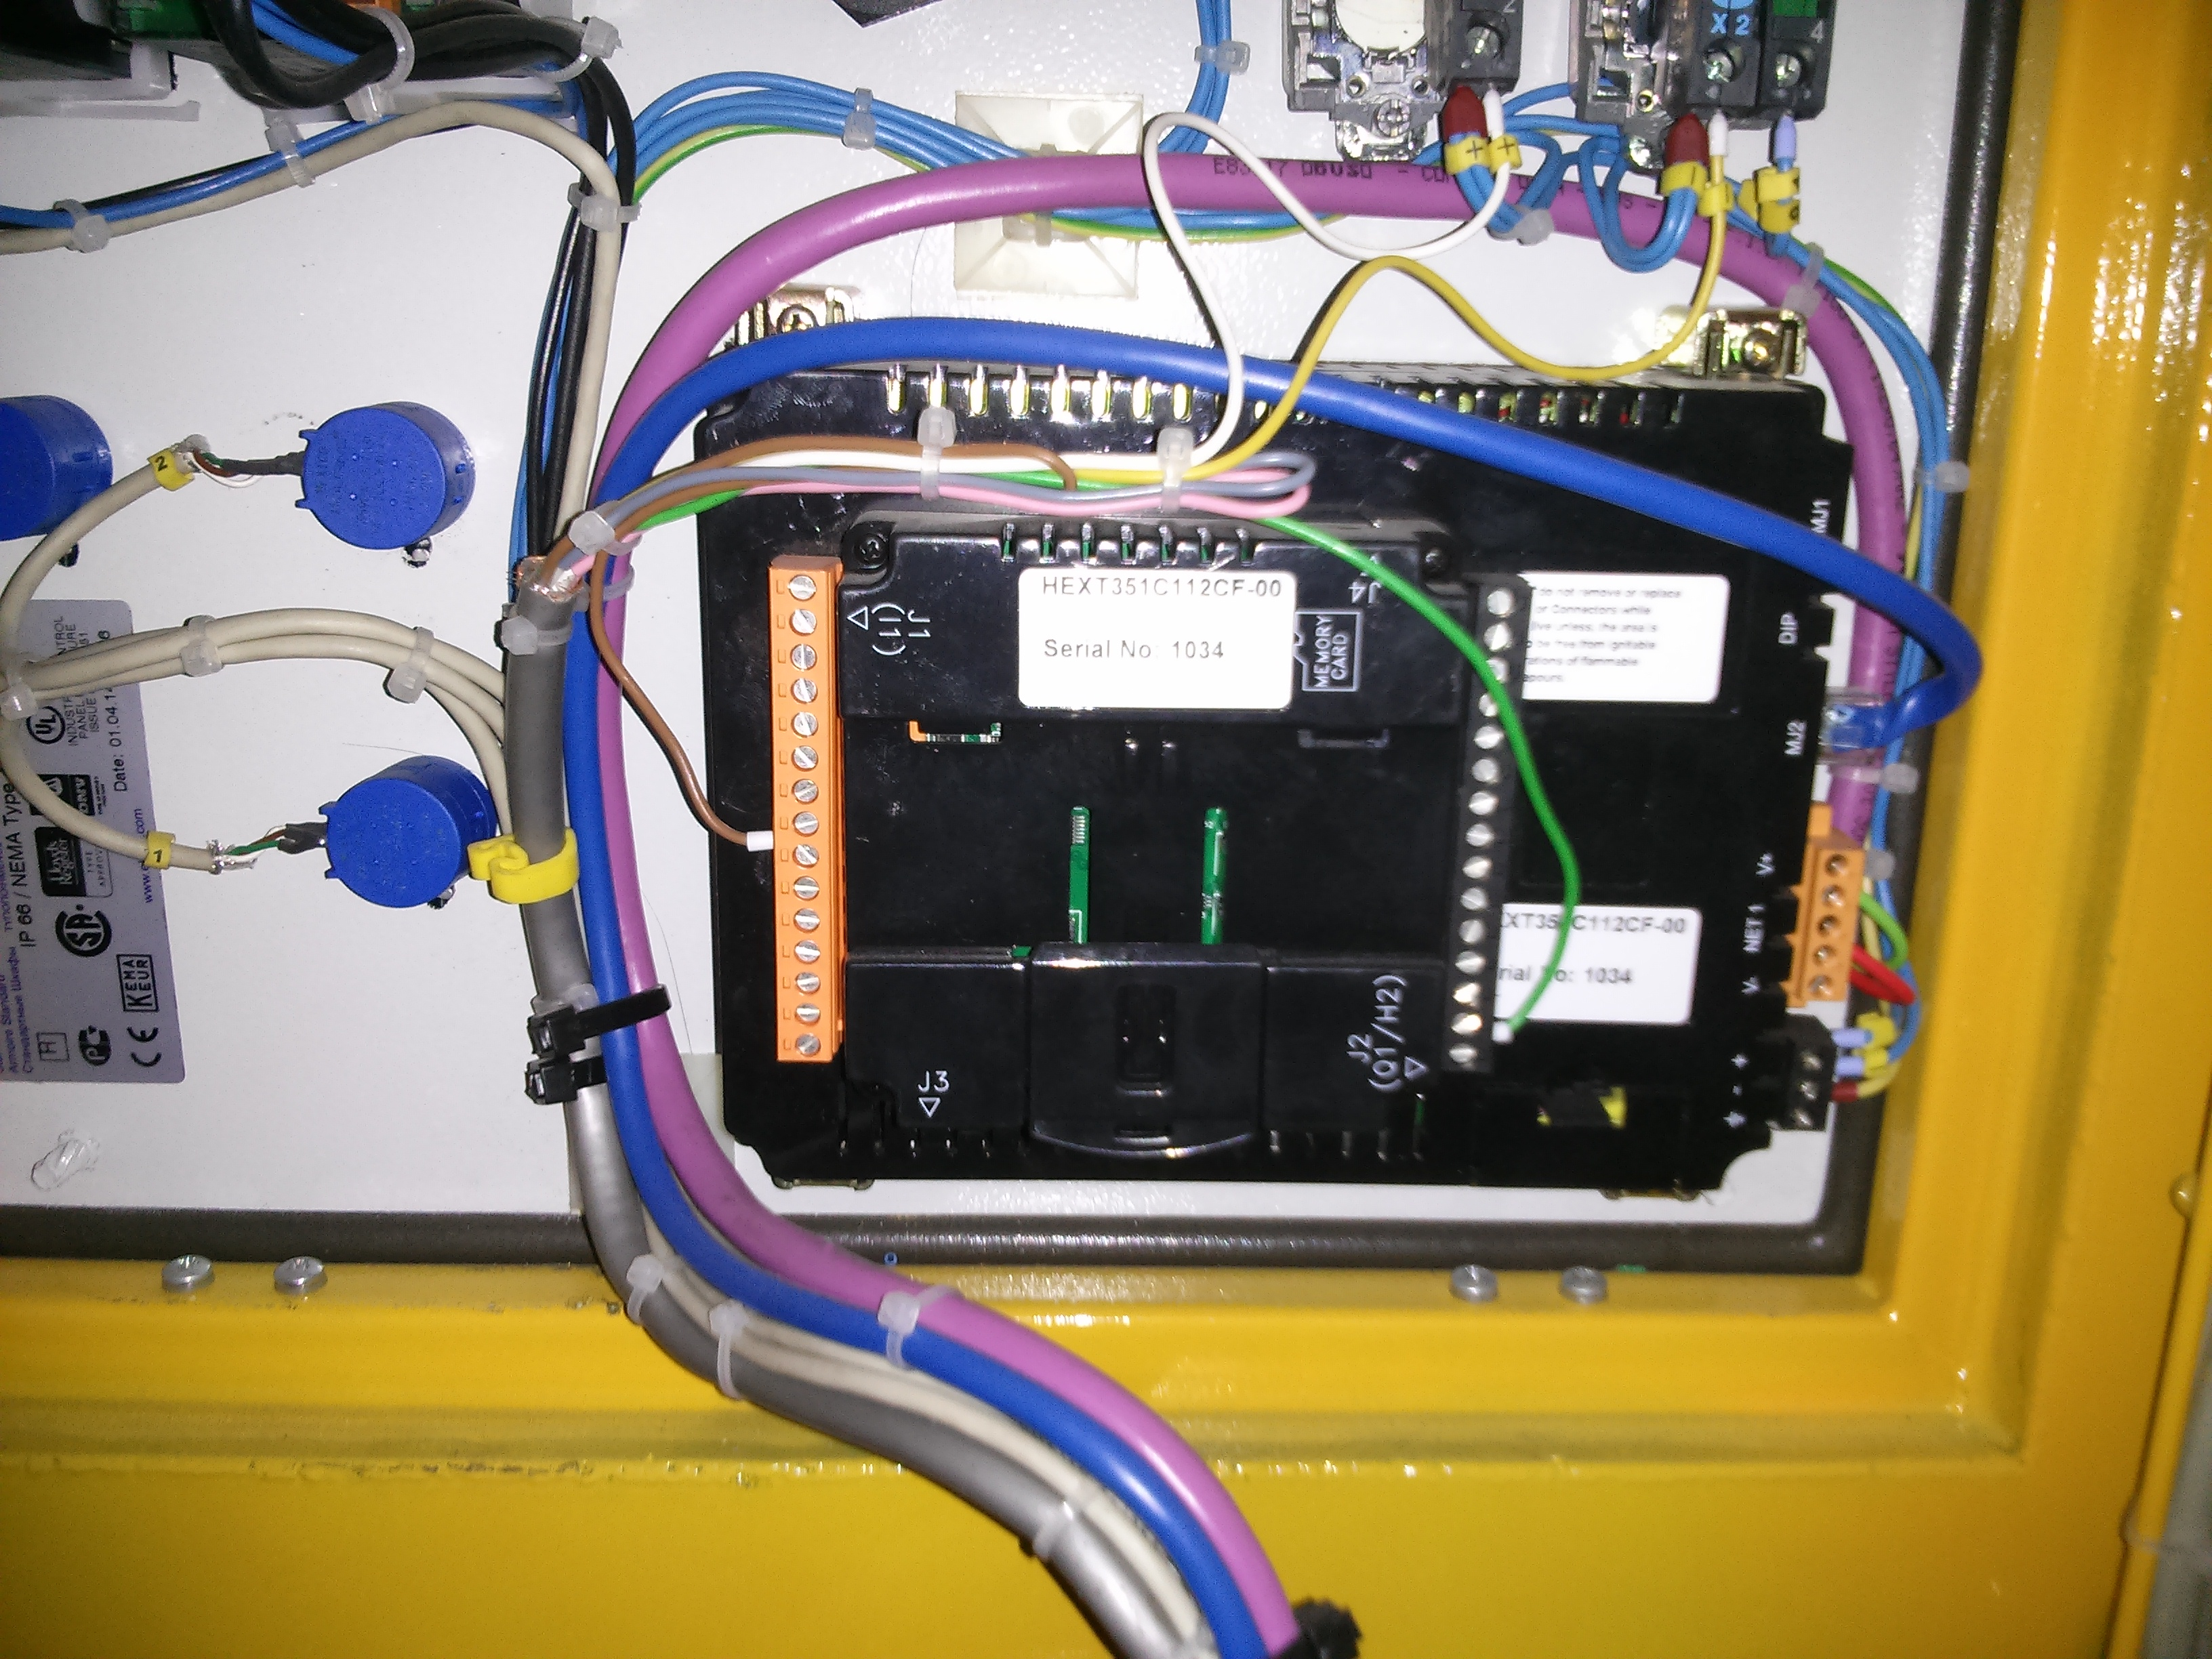
\includegraphics[width=0.4\textwidth]{images/huesca/IMG_20141216_175108.jpg}
            \caption{Pantalla HMI}
            \label{fig:hardware_HMI}
    \end{figure}

     \begin{figure}[H]
            \centering
            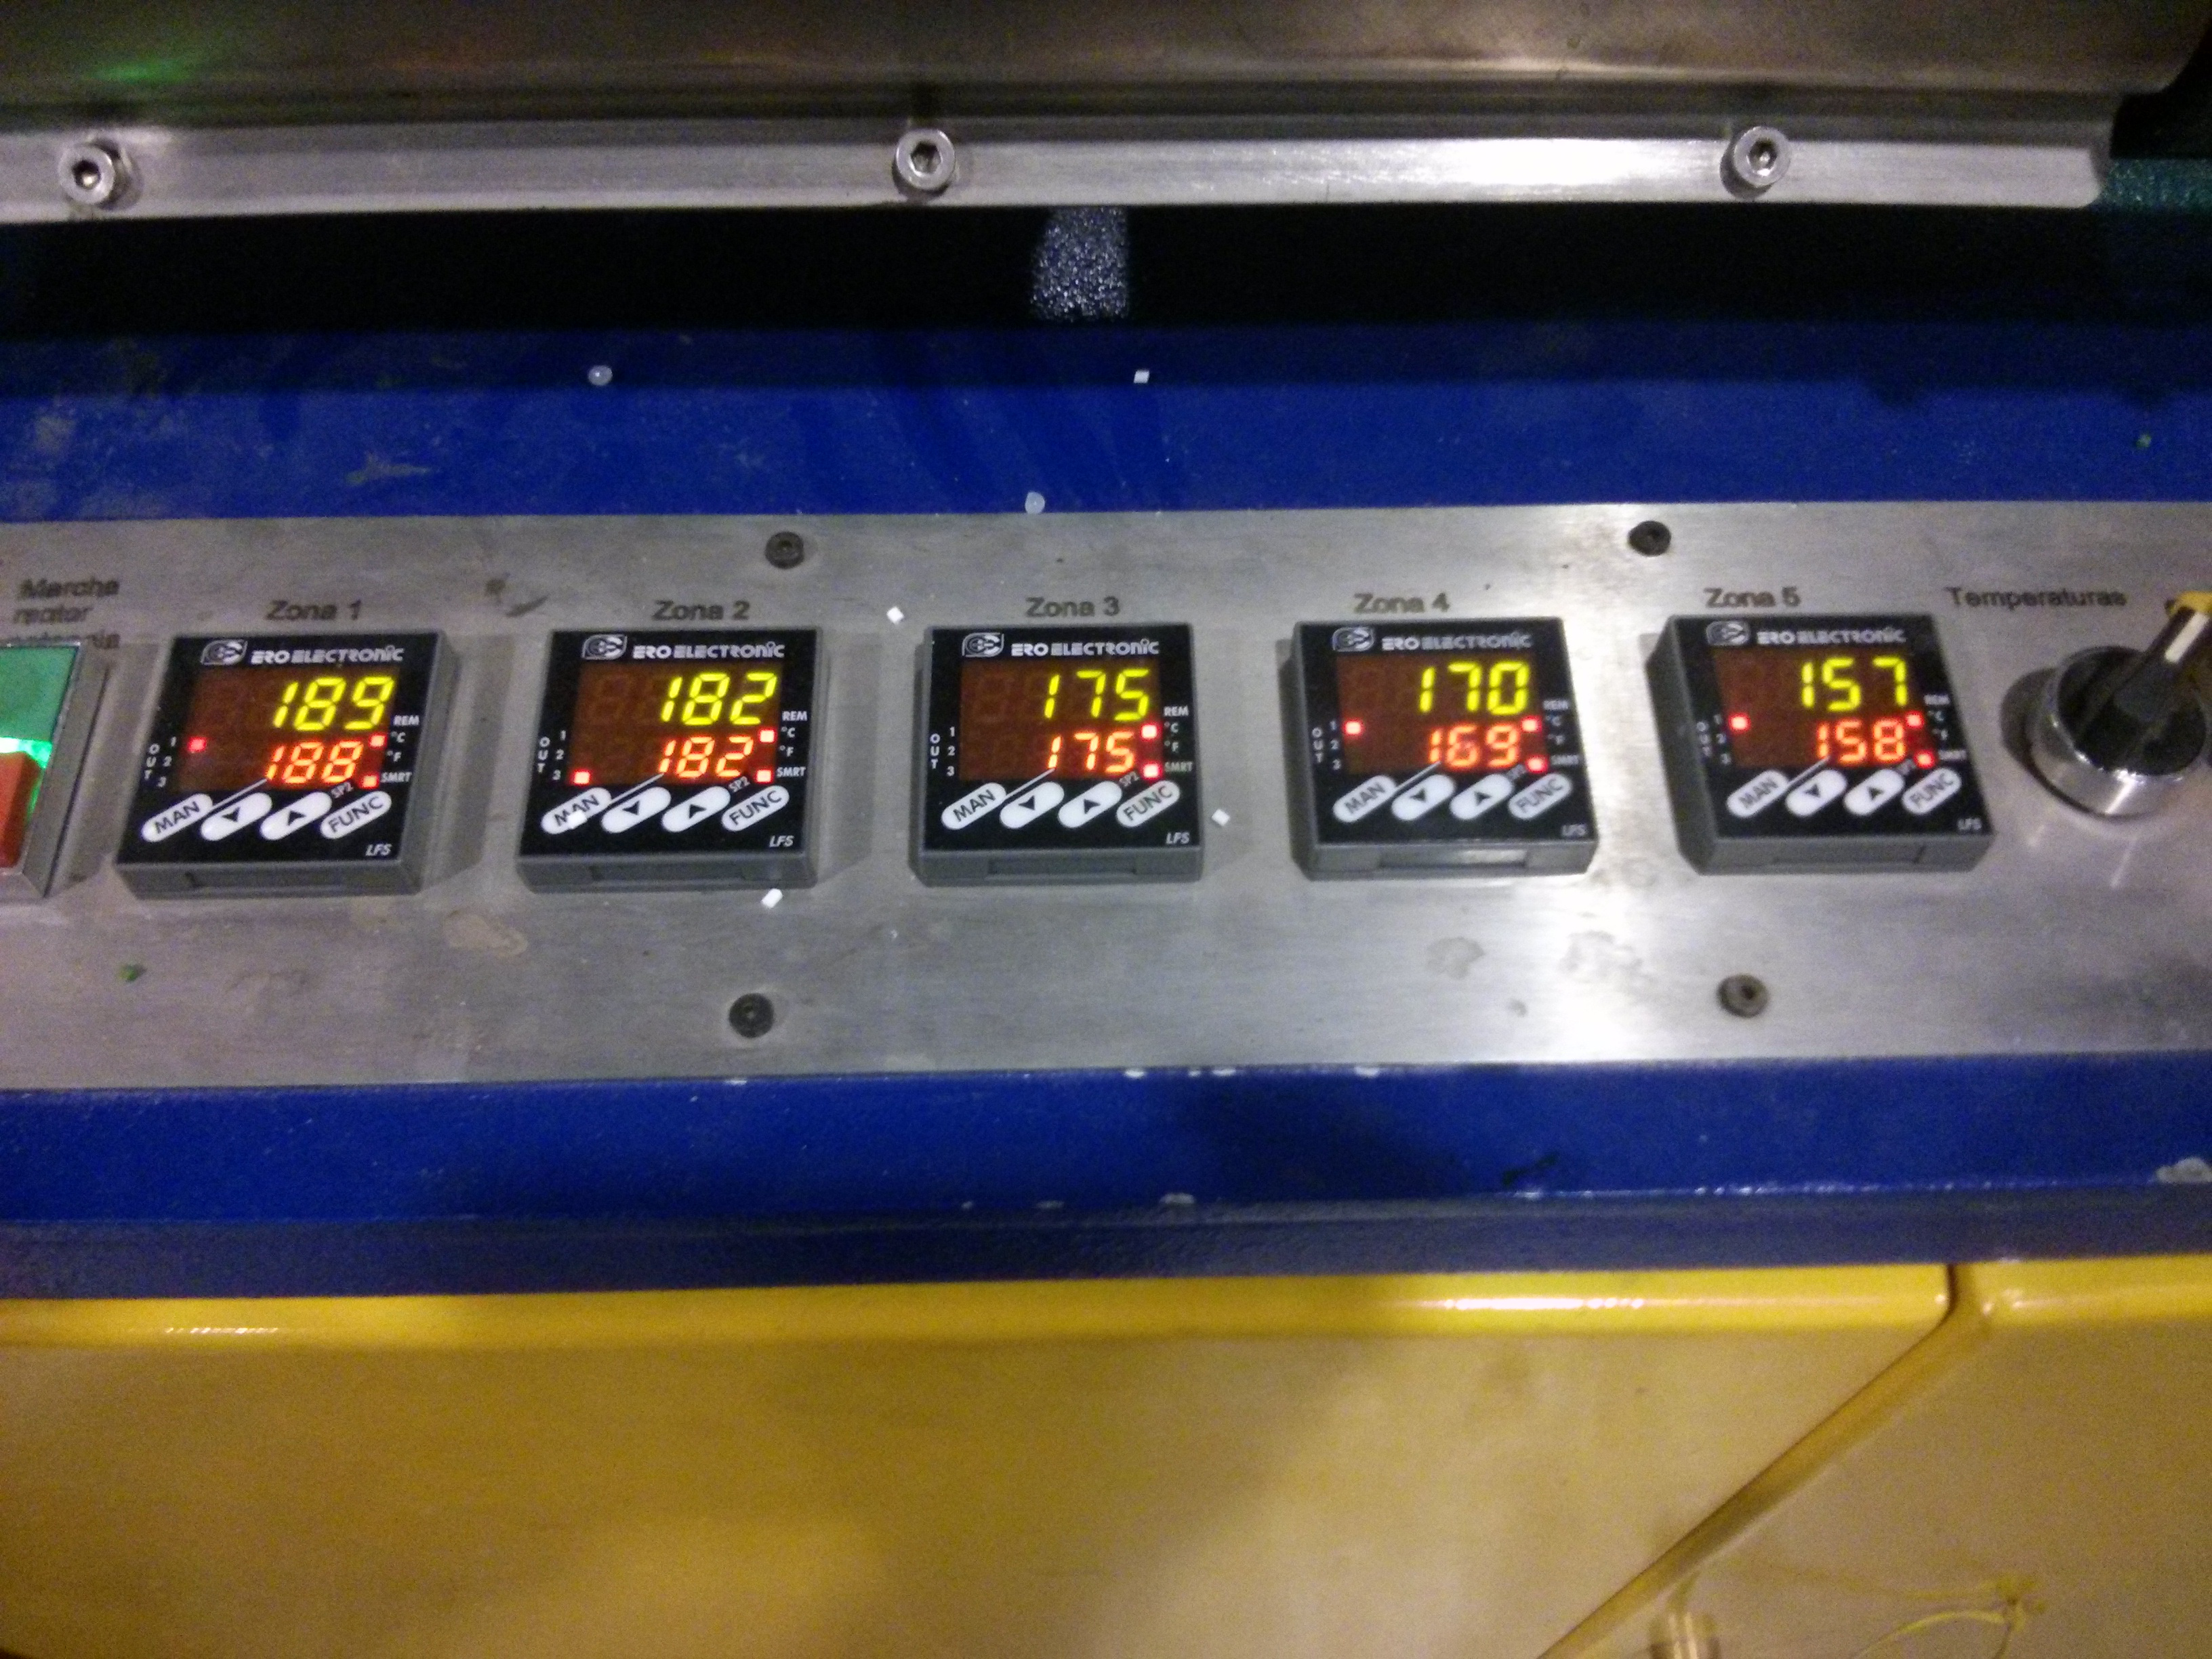
\includegraphics[width=0.4\textwidth]{images/huesca/IMG_20141216_175204.jpg}
            \caption{Sensores de temperatura}
            \label{fig:hardware_temperatura}
    \end{figure}

Buscando en internet referencias de los posibles componentes que disponemos, y con ayuda de los responsables de la fábrica, llegamos a la conclusión de que el hardware que disponemos es el siguiente:

\begin{itemize}
	\item \textbf{Reguladores temperatura Extrusora:} 5x Eroelectronic LFS
	\item \textbf{Regulador temperatura bañera:} 1x OMRON E5CC
	\item \textbf{Bobinadora: IO distribuidas: }
	\begin{itemize}

       \item {SmartStix I/O:} HE559DQM706B y HE559DI710B
       \item{HMI:} HE-XT351C112CF
        \item{Variador (control tractora):} Optidrive rrp2 ODP-24400-SP
        \item{Sensor diámetro:} conectado a módulo Adam 6066
        	\begin{itemize}
        				\item Omron ZX-GIF41 (RS232)
        				\item Omron ZX-GTC41 (Controlador)
                        \item Omron ZX-GT28S41 (sensor)
             \end{itemize}
        \item Relés: OMRON MY2IN
    \end{itemize}
\end{itemize}

Así mismo, disponemos de los datasheet y sabemos qué tipo de comunicación podemos disponer con cada uno, información necesaria para poder establecer la arquitectura del sistema.

\section{Arquitectura planteada}
\label{arquitectura}

Antes de plantear la arquitectura, deberemos establecer el protocolo de comunicaciones y el medio físico por el que irán conectados entre sí. El protocolo establece las reglas necesarias para que dos dispositivos se comuniquen correctamente, haciendo un simil con la realidad, sería el idioma que usan dos personas para hablar. Si dos personas mantienen una conversación en un distinto lenguaje, no se entenderán. Y el medio físico, es cómo se hará la comunicación. Mirando las especificaciones de los componentes llegamos a la siguiente conclusión

\begin{table}[H]

\begin{tabular}{ccc}
\hline
{\bf Dispositivo}     & {\bf Protocolo} & {\bf Medio} \\ \hline
Senores temperatura   & Modbus          & RS485       \\
Pantalla HMI          & Modbus          & RS485       \\
Adam                  & Modbus-TCP      & RS485       \\
Sensor diámetro       & -               & RS232       \\
Variador              & Modbus-TCP      & RS485       \\
Perifería distribuida & CsCAN           & Modbus      \\
Bobinadora            &                 & Cableado    \\ \hline
\end{tabular}
\centering
\caption{Dispositivos disponibles}
\label{tab:dispositivos}
\end{table}

Todos los dispositivos usan protocolos de comunicaciones industriales ampliamente conocidos, como son Modbus y CsCAN. El sensor de diámetro por ejemplo, está conectado a un PC mediante 
RS232, en el que almacena en una base de datos SQLITE (Ver imagen \ref{fig:hardware_sensor_diametro}) las medidas que se van tomando, por ello, será necesario acceder a esa base de datos.
 	\begin{figure}[H]
            \centering
            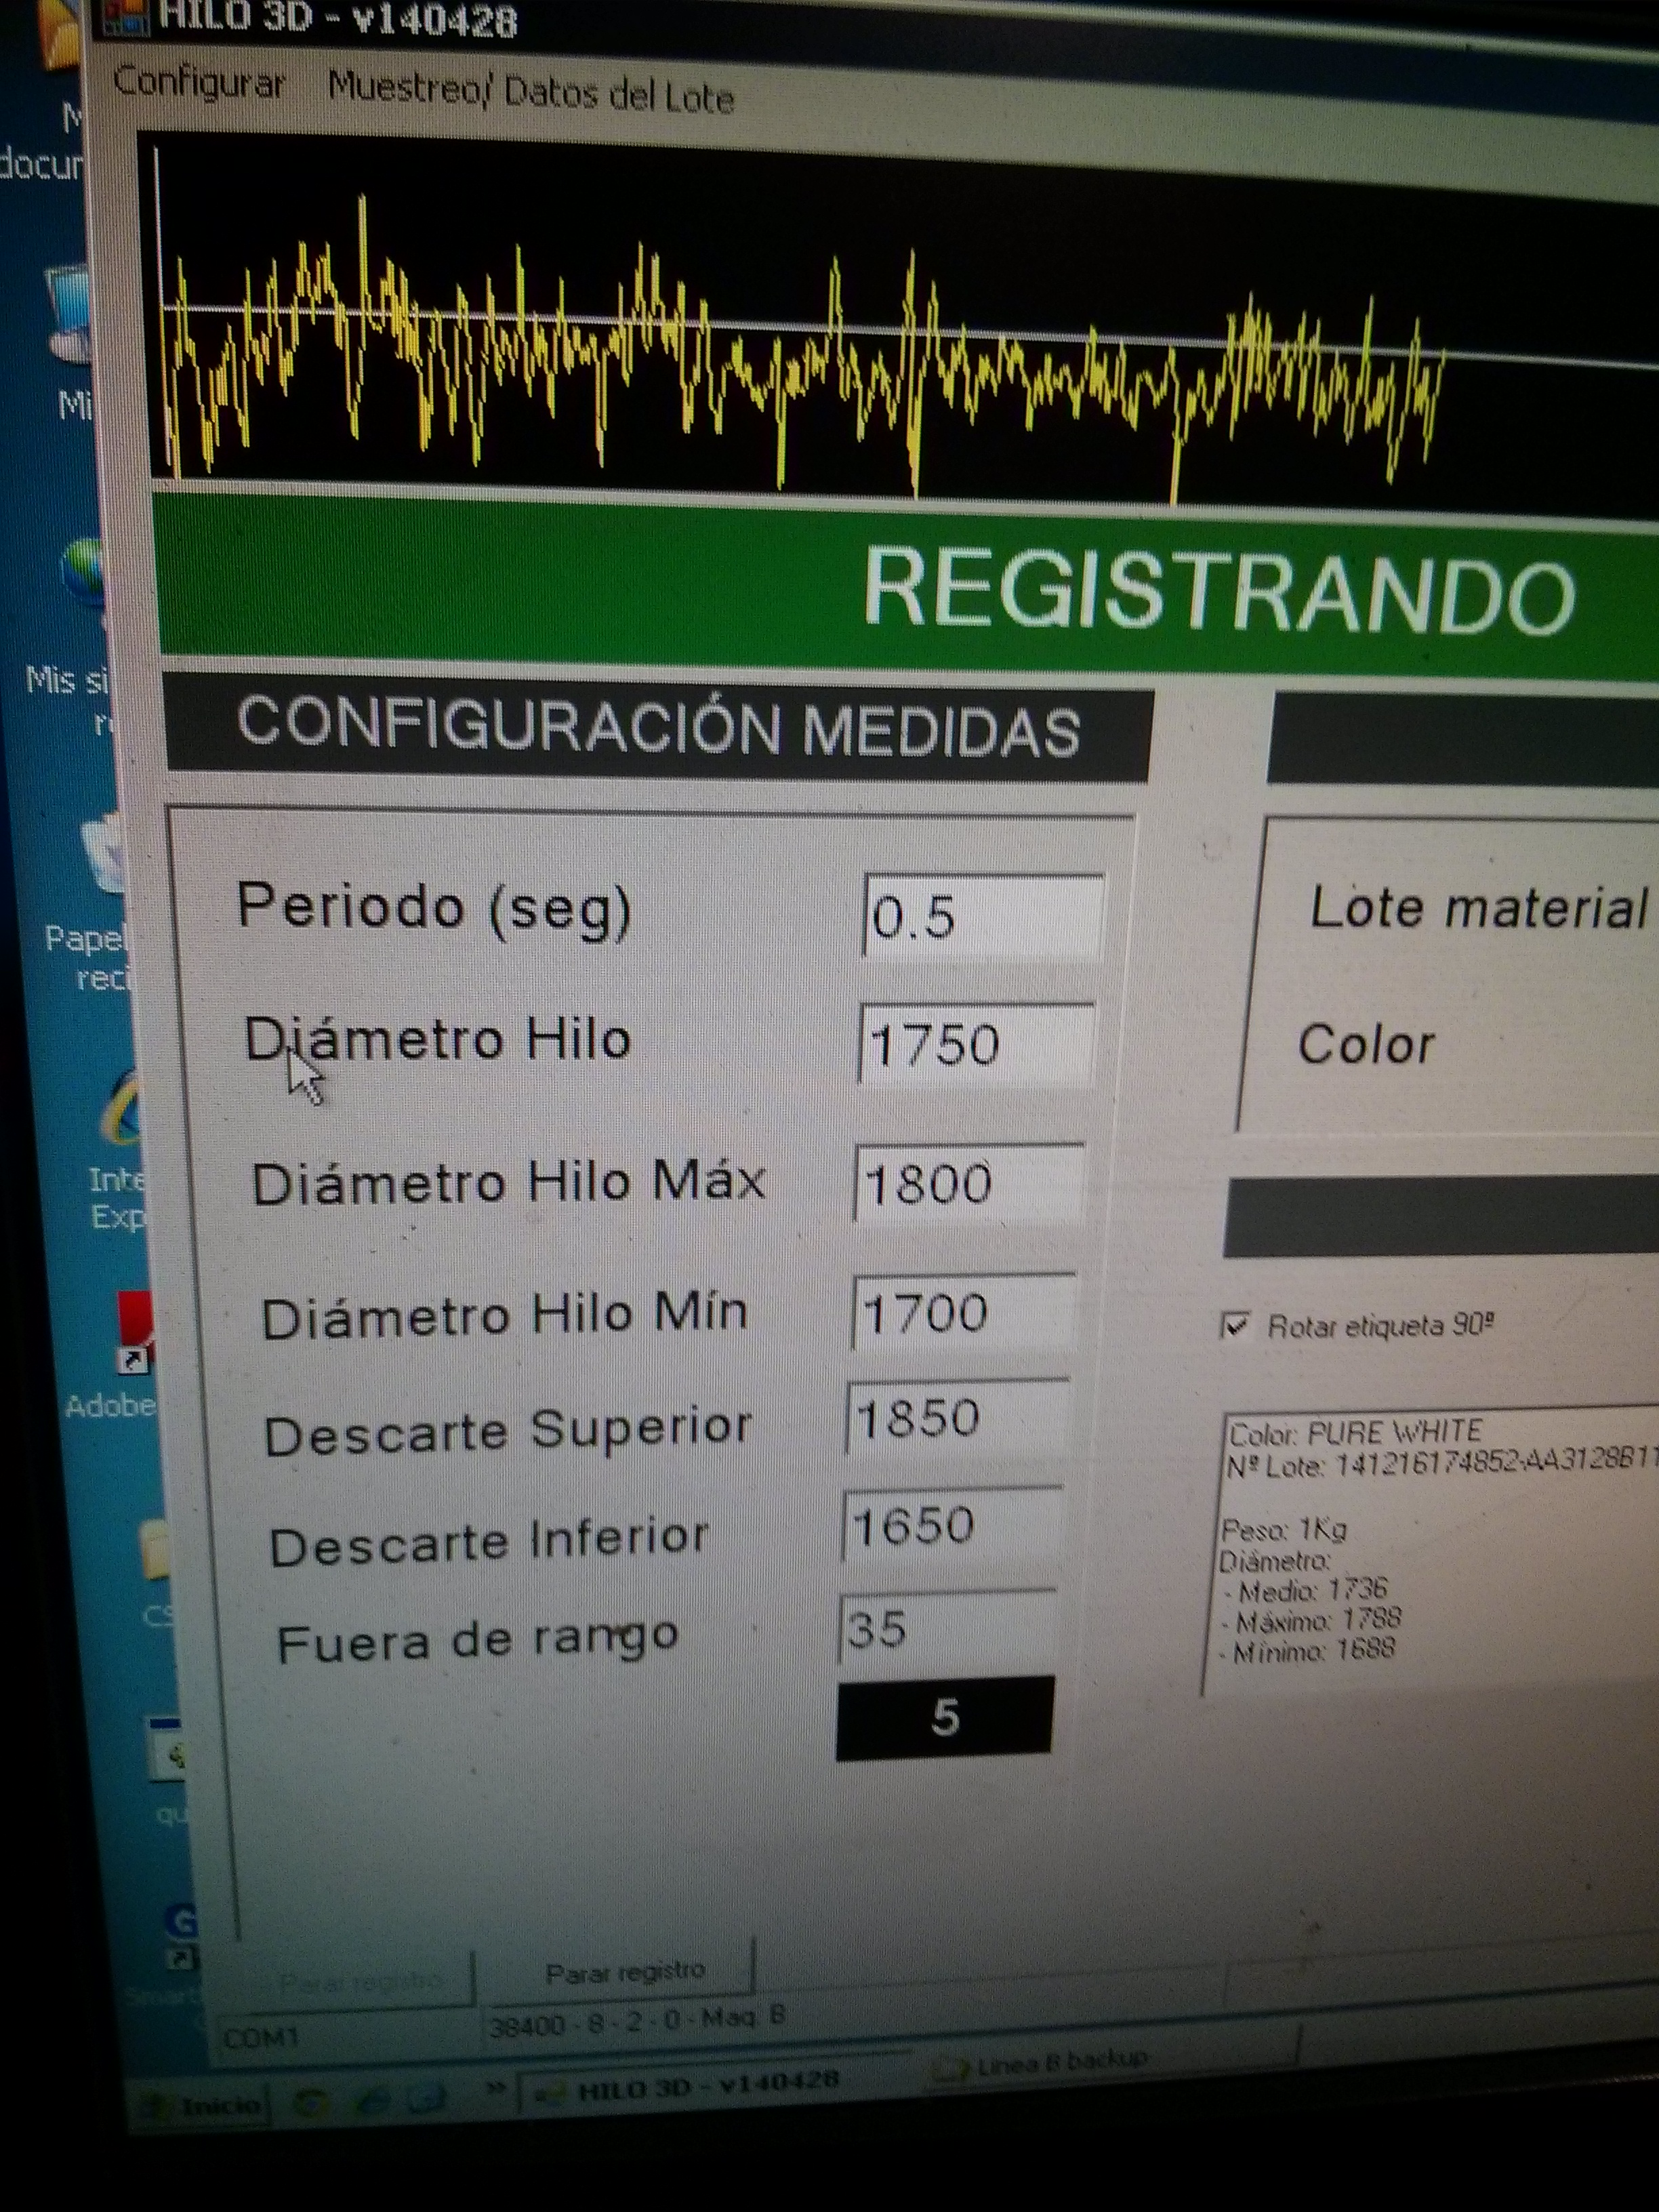
\includegraphics[width=0.5\textwidth]{images/Parametros_adquisicin.jpg}
            \caption{Programa que almacena las medidas tomadas en el sensor de diámetro}
            \label{fig:hardware_sensor_diametro}
    \end{figure}

La bobinadora, no usa ningún protocolo de comunicaciones, mediante señales de entrada salida, ese va realizando la comunicación.\\

Por tanto, con esta información, podemos establecer la arquitectura del sistema.\\

 	\begin{figure}[H]
            \centering
            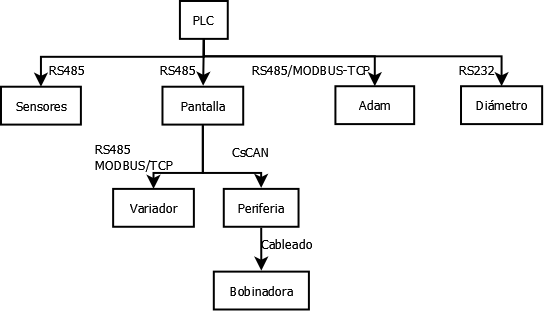
\includegraphics[width=0.6\textwidth]{images/20141229.png}
            \caption{Arquitectura propuesta}
            \label{fig:hardware_arquitectura}
    \end{figure}

Debemos buscar por tanto, un PLC que cumpla con las siguientes especificaciones:

% Please add the following required packages to your document preamble:
% \usepackage{multirow}
\begin{table}[H]
\centering
\begin{tabular}{|c|c|c|}
\hline
\textbf{Característica }                              & \textbf{Descripción}            & \textbf{Cantidad} \\ \hline
\multirow{3}{*}{Comunicaciones industriales} & Ethernet               & 1        \\ \cline{2-3} 
                                             & RS485                  & 1        \\ \cline{2-3} 
                                             & RS232                  & 1        \\ \hline
Software                                     & Acceso R/W a tabla SQL &          \\ \hline
Almacenamiento externo                       & USB o SD               & 1        \\ \hline
\multirow{2}{*}{Periferia digital}           & Entrada                & 8        \\ \cline{2-3} 
                                             & Salida                 & 0        \\ \hline
\multirow{2}{*}{Periferia analógica}         & Entrada                & 4        \\ \cline{2-3} 
                                             & Salida                 & 1        \\ \hline
\end{tabular}
\caption{Especificaciones PLC}
\label{tab:espc_plc}
\end{table}

\section{Elección del PLC}
\label{eleccion_PLC}

Se va a buscar un automáta programable (PLC) que cumpla las especificacione de la tabla \ref{tab:espc_plc}, también se intentará buscar una marca que nos ofrezca las siguientes ventajas, no siendo estas imprescindibles, pero si ayudarán a la hora de elegir un modelo u otro:

\begin{itemize}
		\item{Licencia de desarrollo libre.}
		\item{Modelo básico con el mayor número de especificaciones necesarias.}
		\item{Capacidad de expansión de las características por medio de módulos.}
\end{itemize}

De este modo, conseguiremos reducir el coste total del proyecto. Partiendo de estos requisitos y buscando distintos proveedores por internet, las empresas que mejor se ajustan son:

\begin{itemize}
		\item{\textbf{UNITRONICS:} La compañía ofrece un PLC con pantalla HMI de bajo coste, que es idoneo para pequeños proyectos que no requieran demasiada capacidad. El principal problema es que no dispone de ningúna expansión para almacenar en tarjetas SD, ni se tiene conocimiendo de qu se pueda conectar a una bas de datos MYSQL de forma directa.}
		\item{\textbf{WAGO:} Cumple todos los requisitos que necesitamo, sin embargo, es necesario pagar una licencia para poder usar el software disponible}
		\item{\textbf{ABB:} El PLC de la gama eco trae de serie la mayoría de las cosas que necesitamos, además, si no se superan ciertas limitaciones, no es necesario pagar una licencia para poder usar el software de desarrollo.}
\end{itemize}

Se habla con cada uno de los distribuidores que ofrecen los productos en españa, pidiendo un presupuesto con el material necesario para suplir las necesidades del proyecto:

\begin{table}[H]
\centering
\begin{tabular}{cc}
{\bf Distribuidor} & {\bf Precio (\euro{})} \\ \hline
Unitronics         & 390              \\
Wago               & 1374             \\
Abb                & 506              \\ \hline
\end{tabular}
\caption{Presupuestos de los tres distribuidores}
\label{tab:presupuestos}
\end{table}


Debido al alto presupuesto que nos propuso Wago se descartó, ya que en una primera aproximación, se eligio por que ofrecian alternativas baratas a grandes empresas como Siemens y ABB, sin embargo en el caso que nos ocupa y como se puede ver en la tabla \ref{tab:presupuestos} el precio de ABB es muy competitivo. De hecho es la marca que se elije, debido a que el coste con la marca Unitronics no supone un gasto excesivo y la fiabilidad de los automátas y el software que provee es mejor. Además trae de serie un servidor web con el que podremos hacer una interfaz WEB en la que veremos el estado de la fábrica de forma remota. Por ello, el hardware que se decide adquirir es el siguiente:

\begin{itemize}
	\item{PM564-RP-ETH CPU AC500-eCo,128kB,6DI/6DO-R/2AI/1AO, 24VDC. ETH y WEBSERVER. (Requiere: conectores 9+11 polos)}
	\item{AI562 Módulo S500-eCo, 2AI PT100/1000, Ni100/1000, Resist. 150/300 ( Requiere conector 11 polos)}
	\item{MC502 SD Memory Card 512 MB}
	\item{MC503 Adaptador para tarjeta SD de memoria AC500-eCo.}
\end{itemize}

\section{NO SE COMO LLAMARLOOOO}
\label{}

Una vez realizado el pedido del PLC y disponibles los datasheet de los sensores, dede la fábrica de filamento nos informan que no desean continuar con el proyecto y que no nos facilitarán más información acerca del proceso de fabricación. Por ello, el sentido de este proyecto cambia, ya que no podremos tener acceso a los sensores ni ninguna instrumentación de la fábrica.\\

Se decide entonces cambiar el enfoque del proyecto, desde BQ se tiene planes de investigación en lo referente a los polímeros usados en la impresión 3D para poder mejorar en el producto que ofrecen, y hay intención de adquirir dos extrusoras propias:

\begin{itemize}

		\item{Extrusora industrial.}
		\item{Extrusora de laboratorio.}
\end{itemize}

Con cualquiera de estas dos extrusoras se podría implementar el sistema propuesto para este proyecto, sin embargo el principal problema son los tiempos de adquisición que no se tiene planeado comprarlas hasta el último trimestre de 2015, con lo que el plazo de entrega del presente proyecto se alargaría.\\

Podría realizarse el proyecto sin tener ninguno de los materiales, unicamente con el PLC y simuladores del protocolo MODBUS, pero no sería algo completo. En el departamento de robótica e innovación de BQ se dispone de un KIT DIY de una extrusora de filamento, filestruder.\\

	\begin{figure}[H]
            \centering
            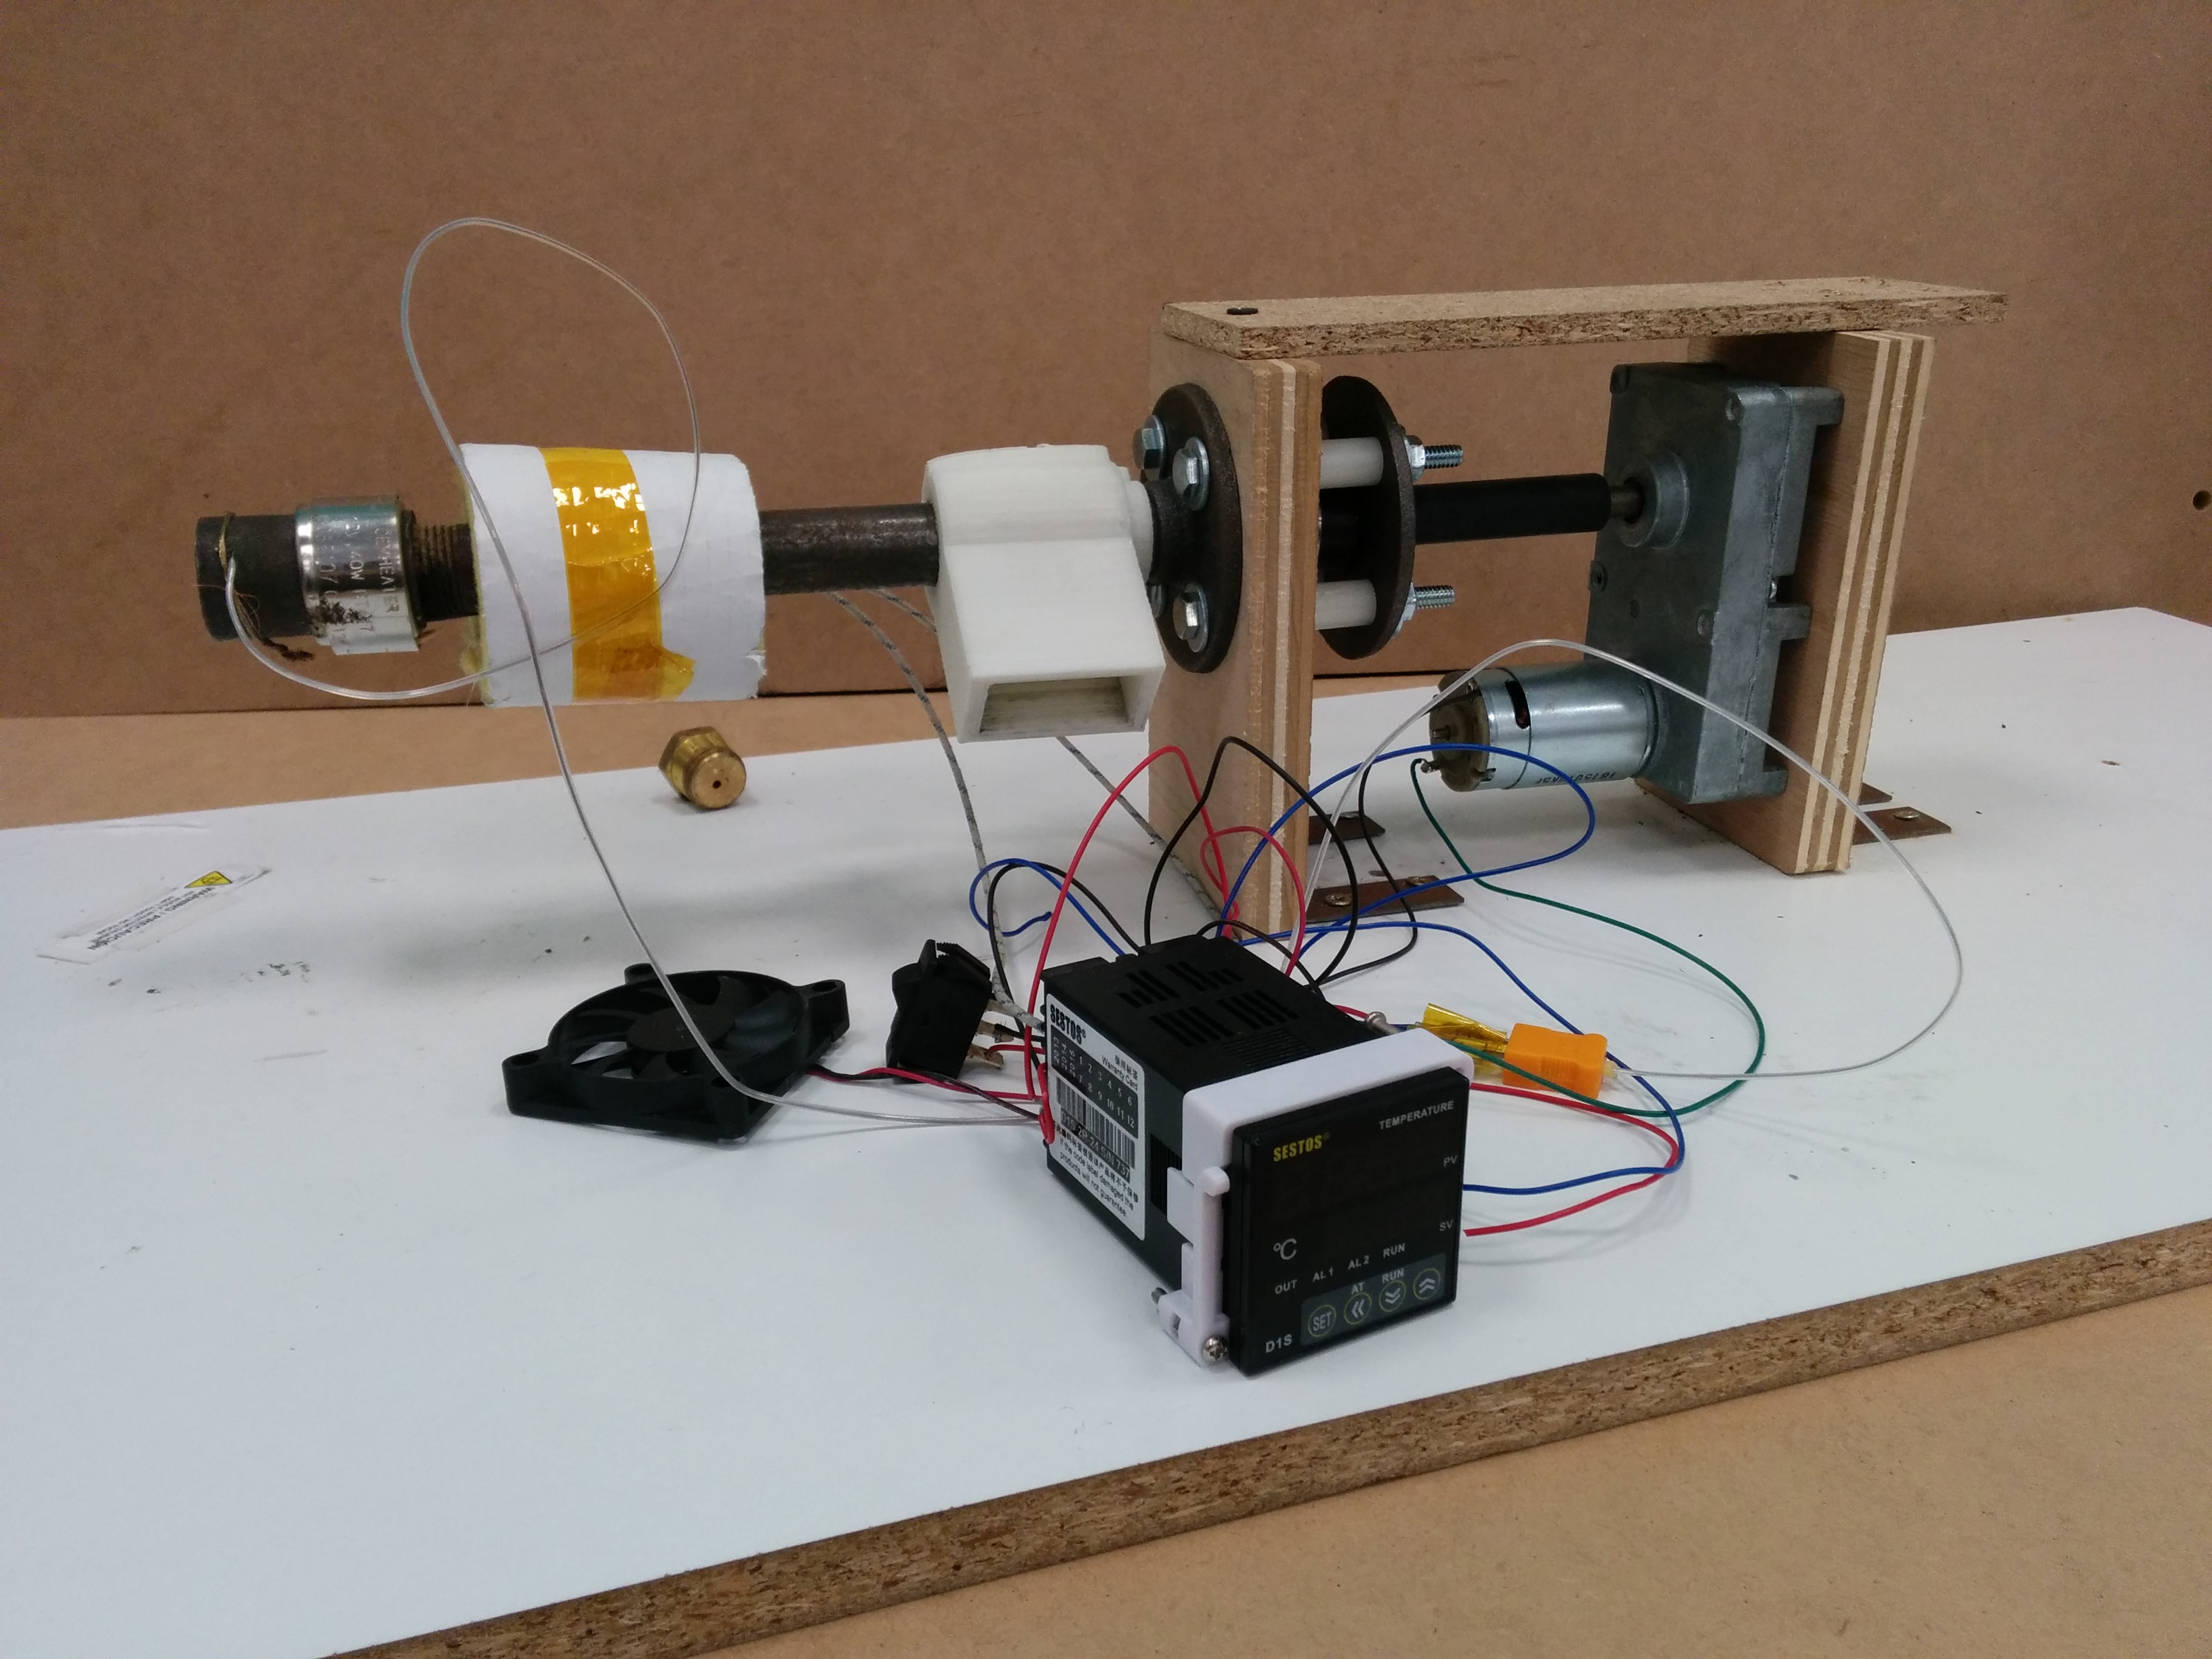
\includegraphics[width=0.6\textwidth]{images/filaextruder/IMG_20150313_111634.jpg}
            \caption{Maqueta de filastruder montada}
            \label{fig:hardware_filastruder}
    \end{figure}


Filastruder se presenta como proyecto en Noviembre de 2012 \cite{filastruder} y consiguió recaudar $212.278 \$$ en una campaña de kickstarter. Es un extrusor de baja capacidad y de bajo coste, liberado como Open Source. Todo el proceso de construcción del extrusor se documento en el foro y se creó una comunidad de usuarios interesandos en los extrusores caseros.\\

Algunas de las características de este extrusor son:

\begin{table}[H]
\centering

\begin{tabular}{lc}
\textbf{Par de detenimiento del motor}            & $12N.m$                           \\
\textbf{Velocidad del motor}                      & $3 rpm$                           \\
\textbf{Tiempo para extruir 1kg}                  & $24H$                             \\
\textbf{Diámetro del husillo}                     & $15.875mm$                        \\
\textbf{Longitud del husillo}					  & $255mm$           				  \\
\textbf{Tolerancia declarada}					  & $\pm 0.05 mm$					  \\	

\end{tabular}
\caption{Características filastruder. Fuente\cite{tfg_diego}}
\label{tab:caract_filas}
\end{table}

La filastruder que disponemos, trae un controlador PID que mediante una resistencia de potencia y un termopar tipo J, consigue regular la temperatura del dado de la extrusora. Así mismo, trae un motor de continua, con una etapa reductora, para poder mover el husillo y hacer avanzar los pellets de PLA por el cañon.\\

La maqueta lleva parada alrededor de un año y no se sabe muy bien si su funcionamiento es el correcto, por ello, se monta con una fuente de alimentación y se comprueba si al menos es capaz de mover el husillo y calentar el carucho.\\

	\begin{figure}[H]
            \centering
            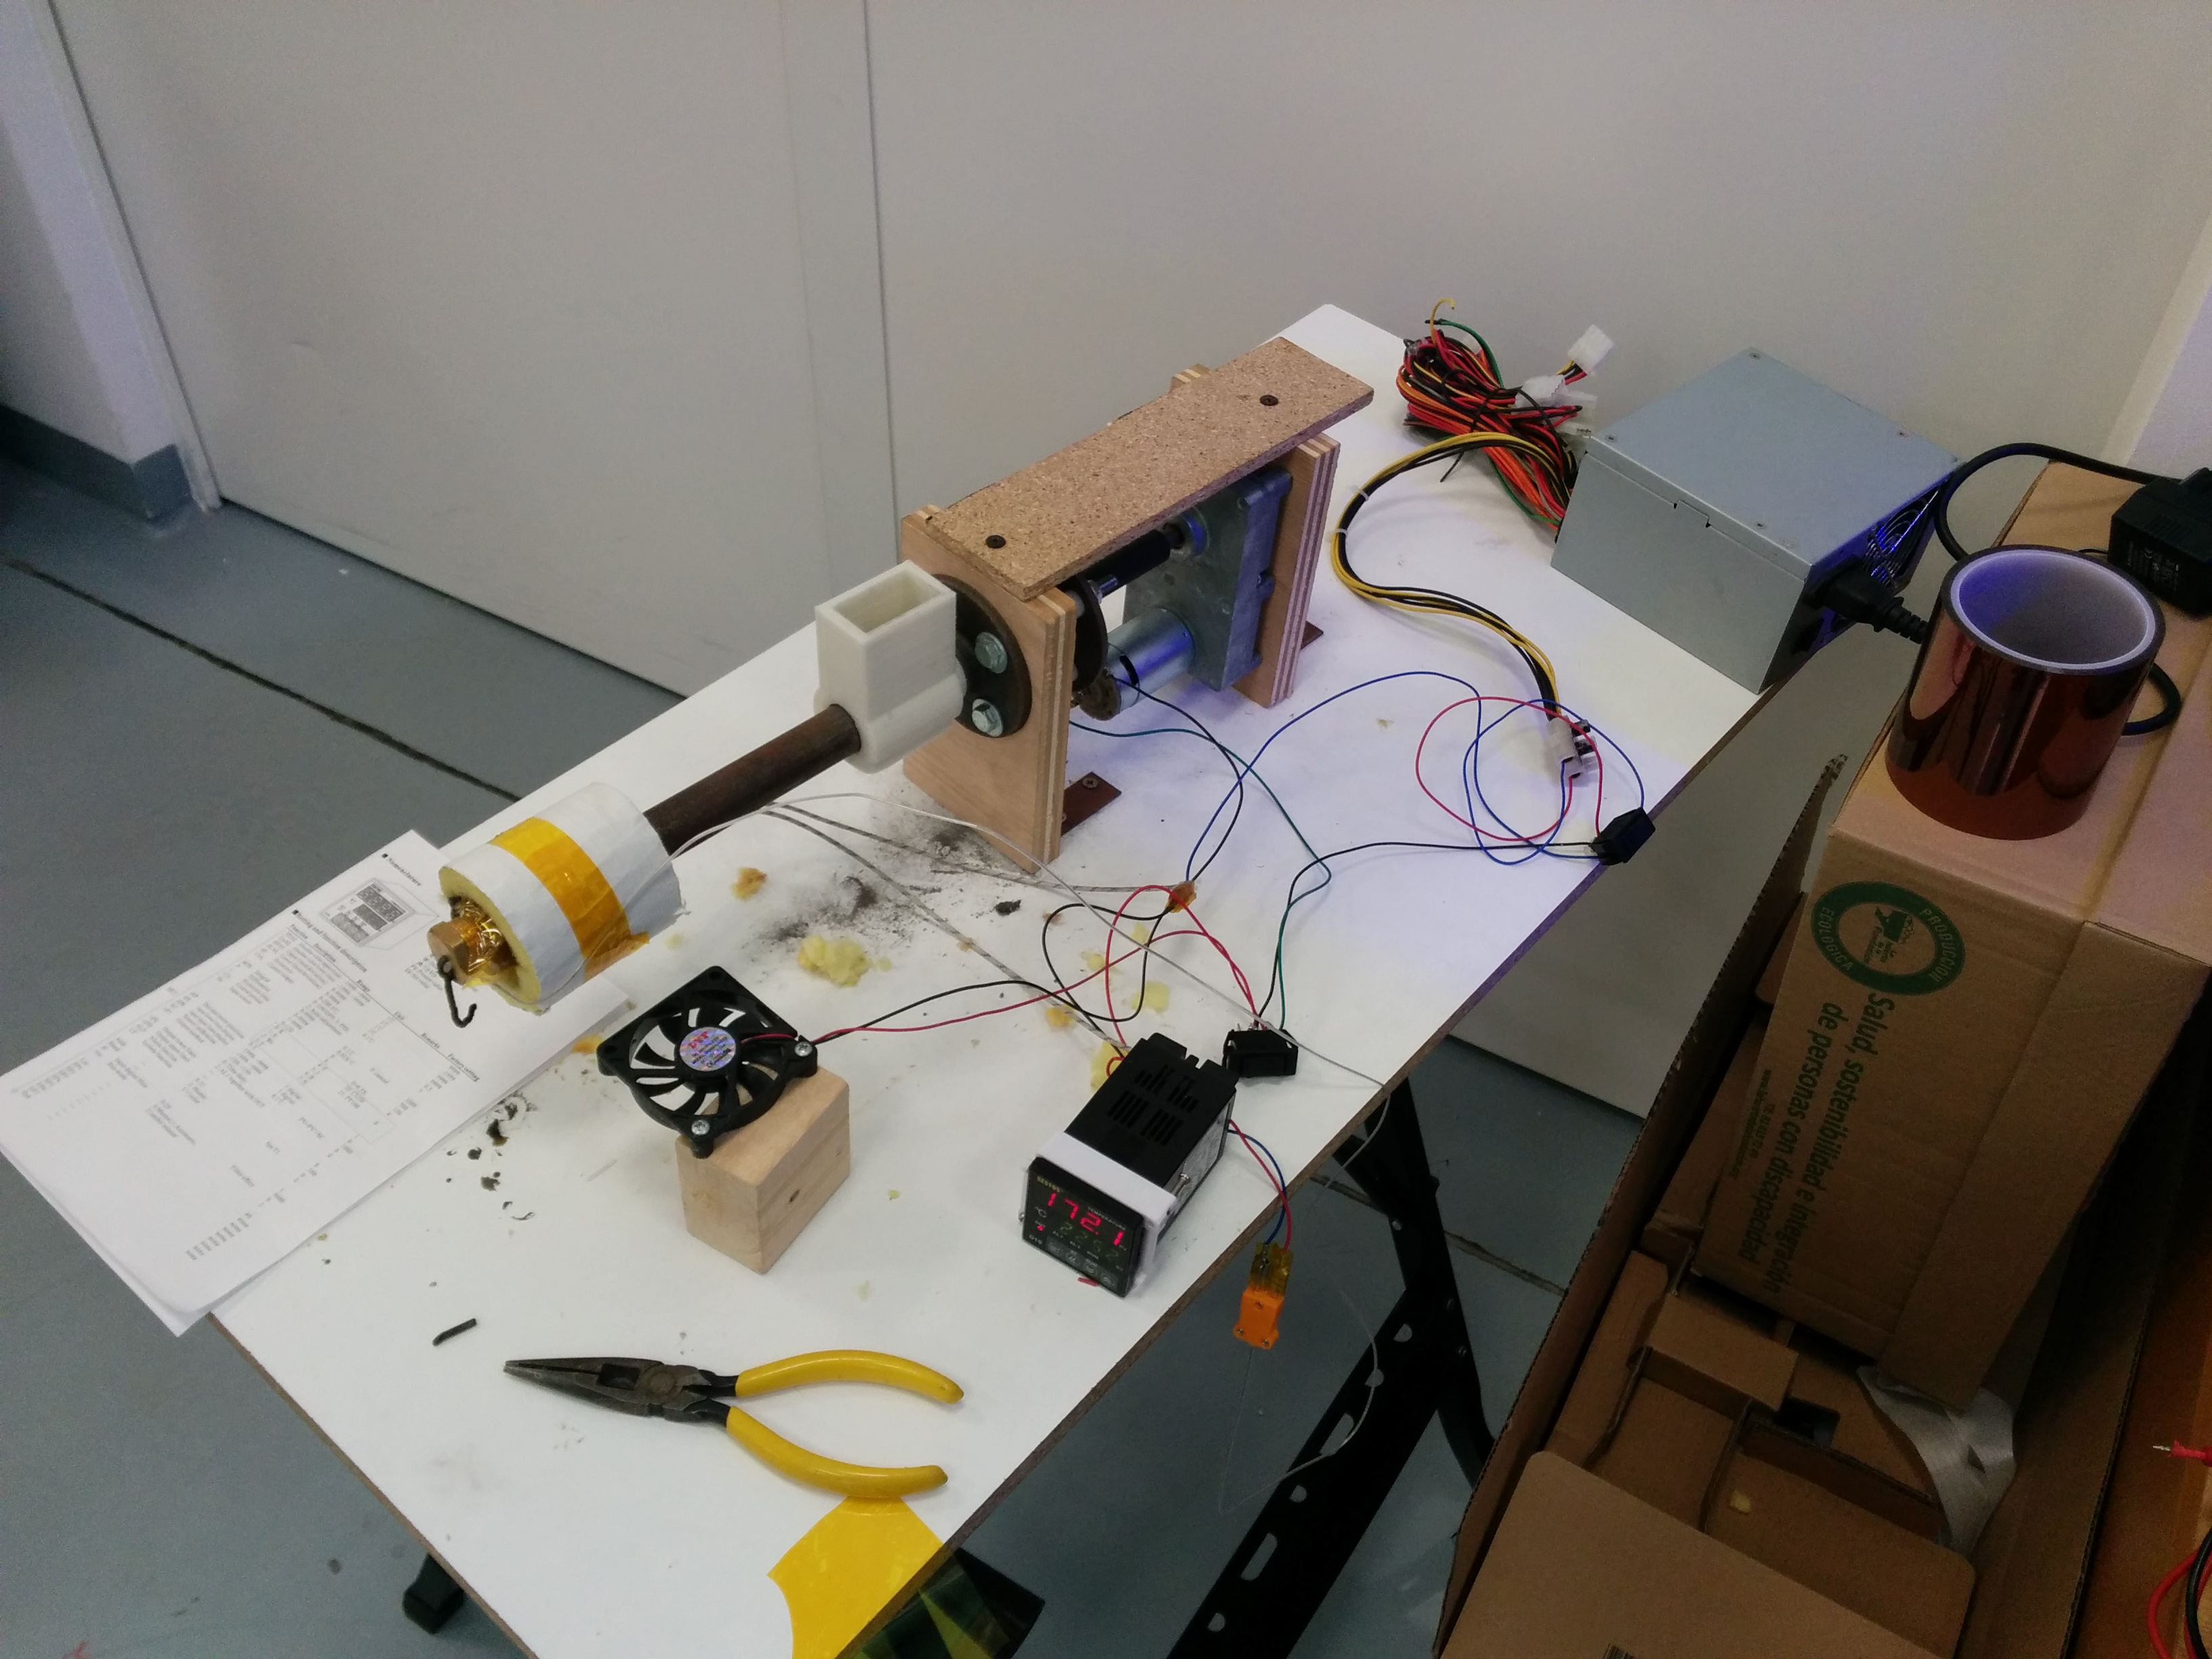
\includegraphics[width=0.6\textwidth]{images/filaextruder/IMG_20150225_093400.jpg}
            \caption{Maqueta de filastruder funcionando}
            \label{fig:hardware_filastruder2}
    \end{figure}
    	\begin{figure}[H]
            \centering
            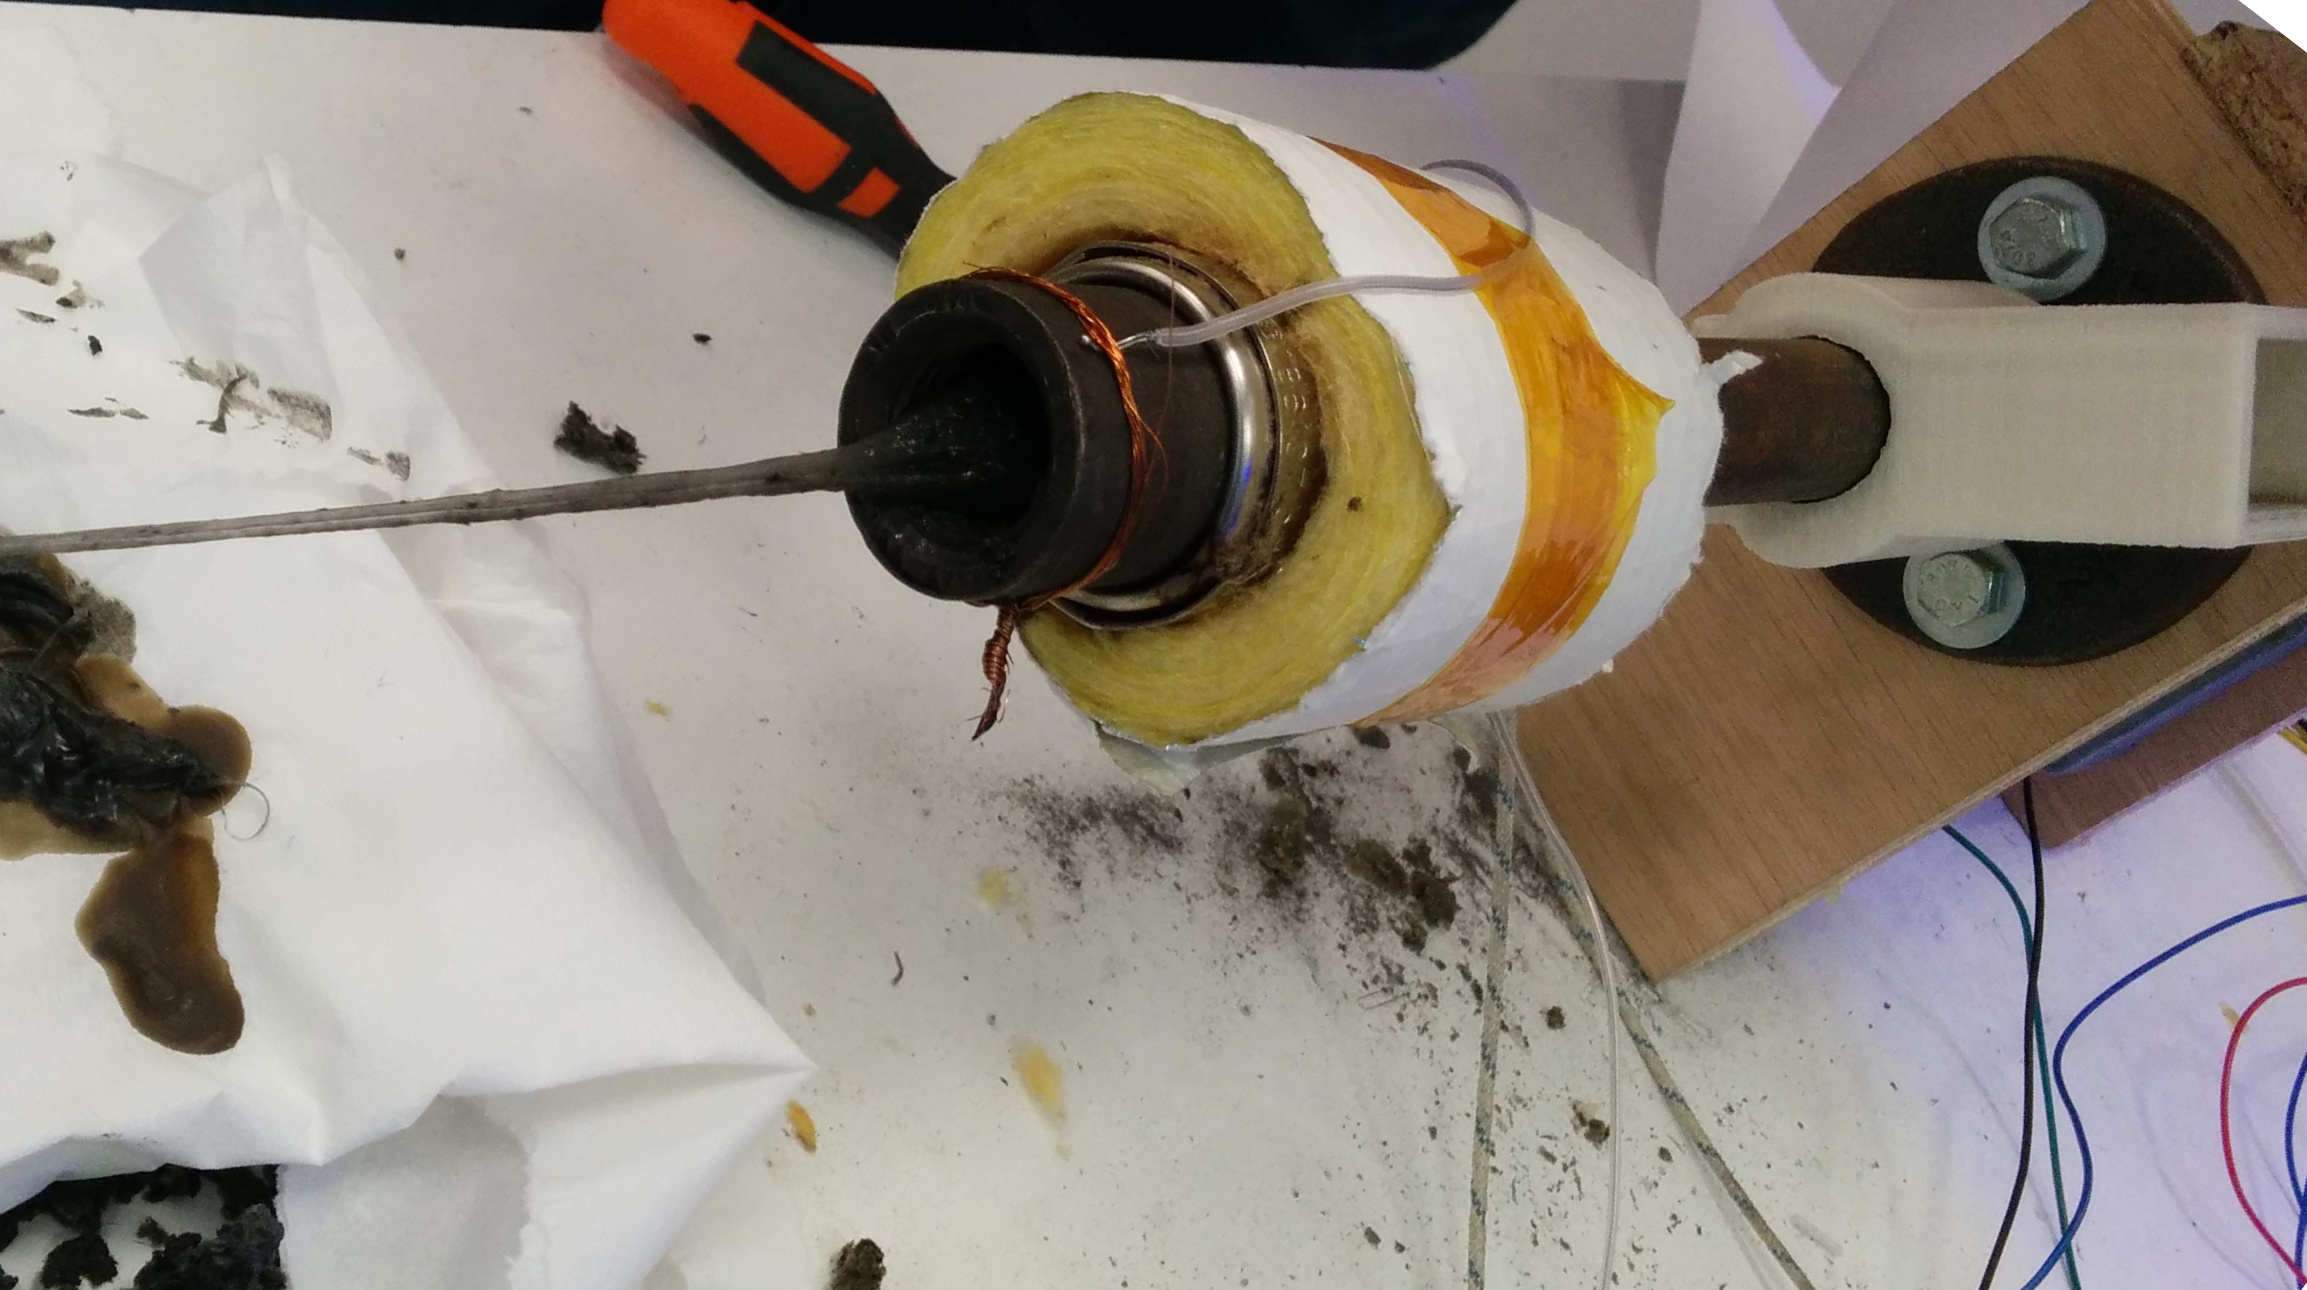
\includegraphics[width=0.6\textwidth]{images/filaextruder/IMG_20150225_124525.jpg}
            \caption{Maqueta de filastruder funcionando}
            \label{fig:hardware_filastruder3}
    \end{figure}

Después de vaciar y limpiar correctamente el cañon, comprobamos que el funcionamiento del filastruder puede sernos útil para al menos hacer un proyecto a escala reducida de lo que originariamente se pensó. Por tanto, los objetivos vistos en el capítulo \ref{cap:objetivos}, página \pageref{cap:objetivos},no cambian.\\

En este punto, tenemos accesibles los materiales necesarios para la realización del proyecto,  así podremos avanzar en el proyecto sin necesidad de pedir permisos a terceras personas,sin embargo se añaden nuevas tareas al proyecto, como la puesta en marcha de nuestra propia extrusora, lo cual añadirá una dificultad extra y hará que la fecha de entrega final se proloongue.\\

\section{Montaje Filastruder}
\label{sec:filastruder}
El control de temperatura del filastruder se realiza mediante un regulador PID modelo Sestos D1S. Conectandole el termopar tipo J y el cartucho calefactor, es capaz de regular la temperatura que deseemos del dado, el único problema es que no dispone de comunicaciones industriales, y sólo se puede introducir la temperatura deseada mediante el display que incorpora.
   	\begin{figure}[H]
            \centering
            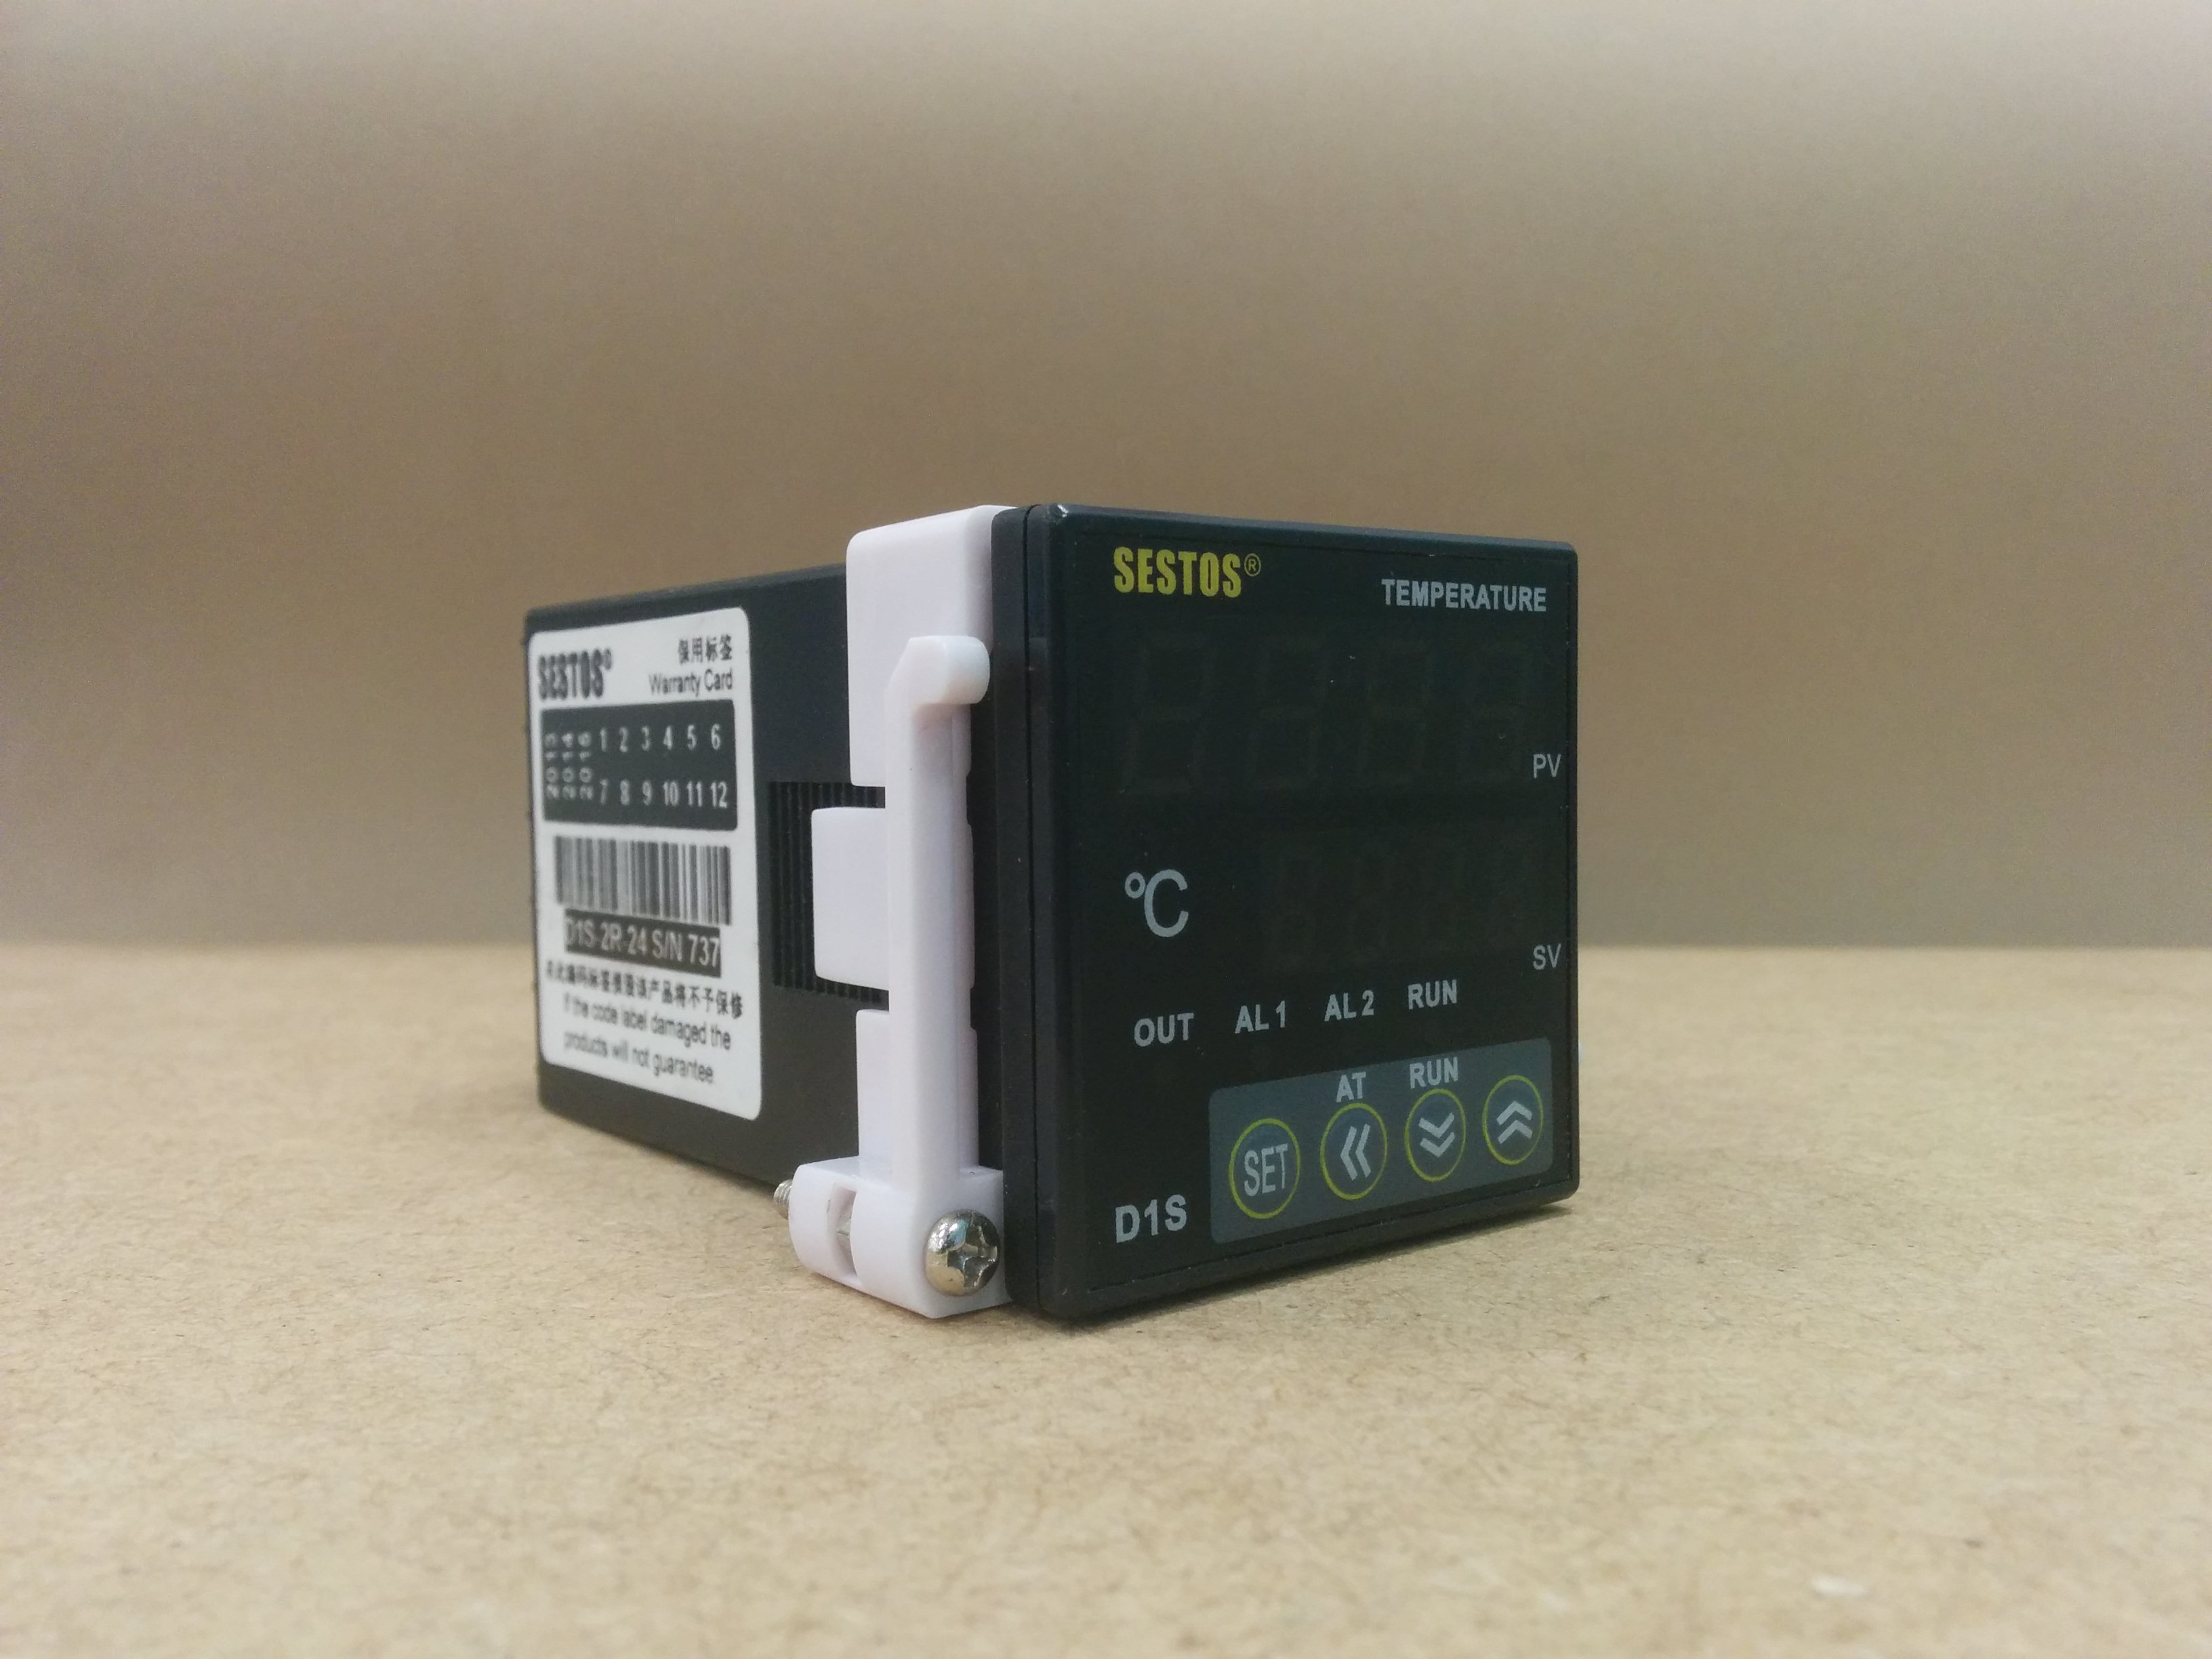
\includegraphics[width=0.6\textwidth]{images/filaextruder/IMG_20150814_123957.jpg}
            \caption{Controlador PID de temperatura Sestos}
            \label{fig:hardware_sestos}
    \end{figure}

Se decide entonces no usar el PID e integrarlo directamente en el PLC ya que, con el hardware que compramos tenemos dos entradas analógicas capaces de leer sensores de temperatura del tipo PT100. De este modo, podremos introducir dos zonas de calentamiento, una en el dado del cañon y otra en la entrada de los pellet para poder tener varios registros de temperaturas como se tenía en la idea principal , que se disponian hasta cinco sensores de temperatura.\\

Se pasa a instalar sobre una plancha de madera la filastruder y todo el cableado futuro que se va a usar a lo largo del proyecto:

   	\begin{figure}[H]
            \centering
            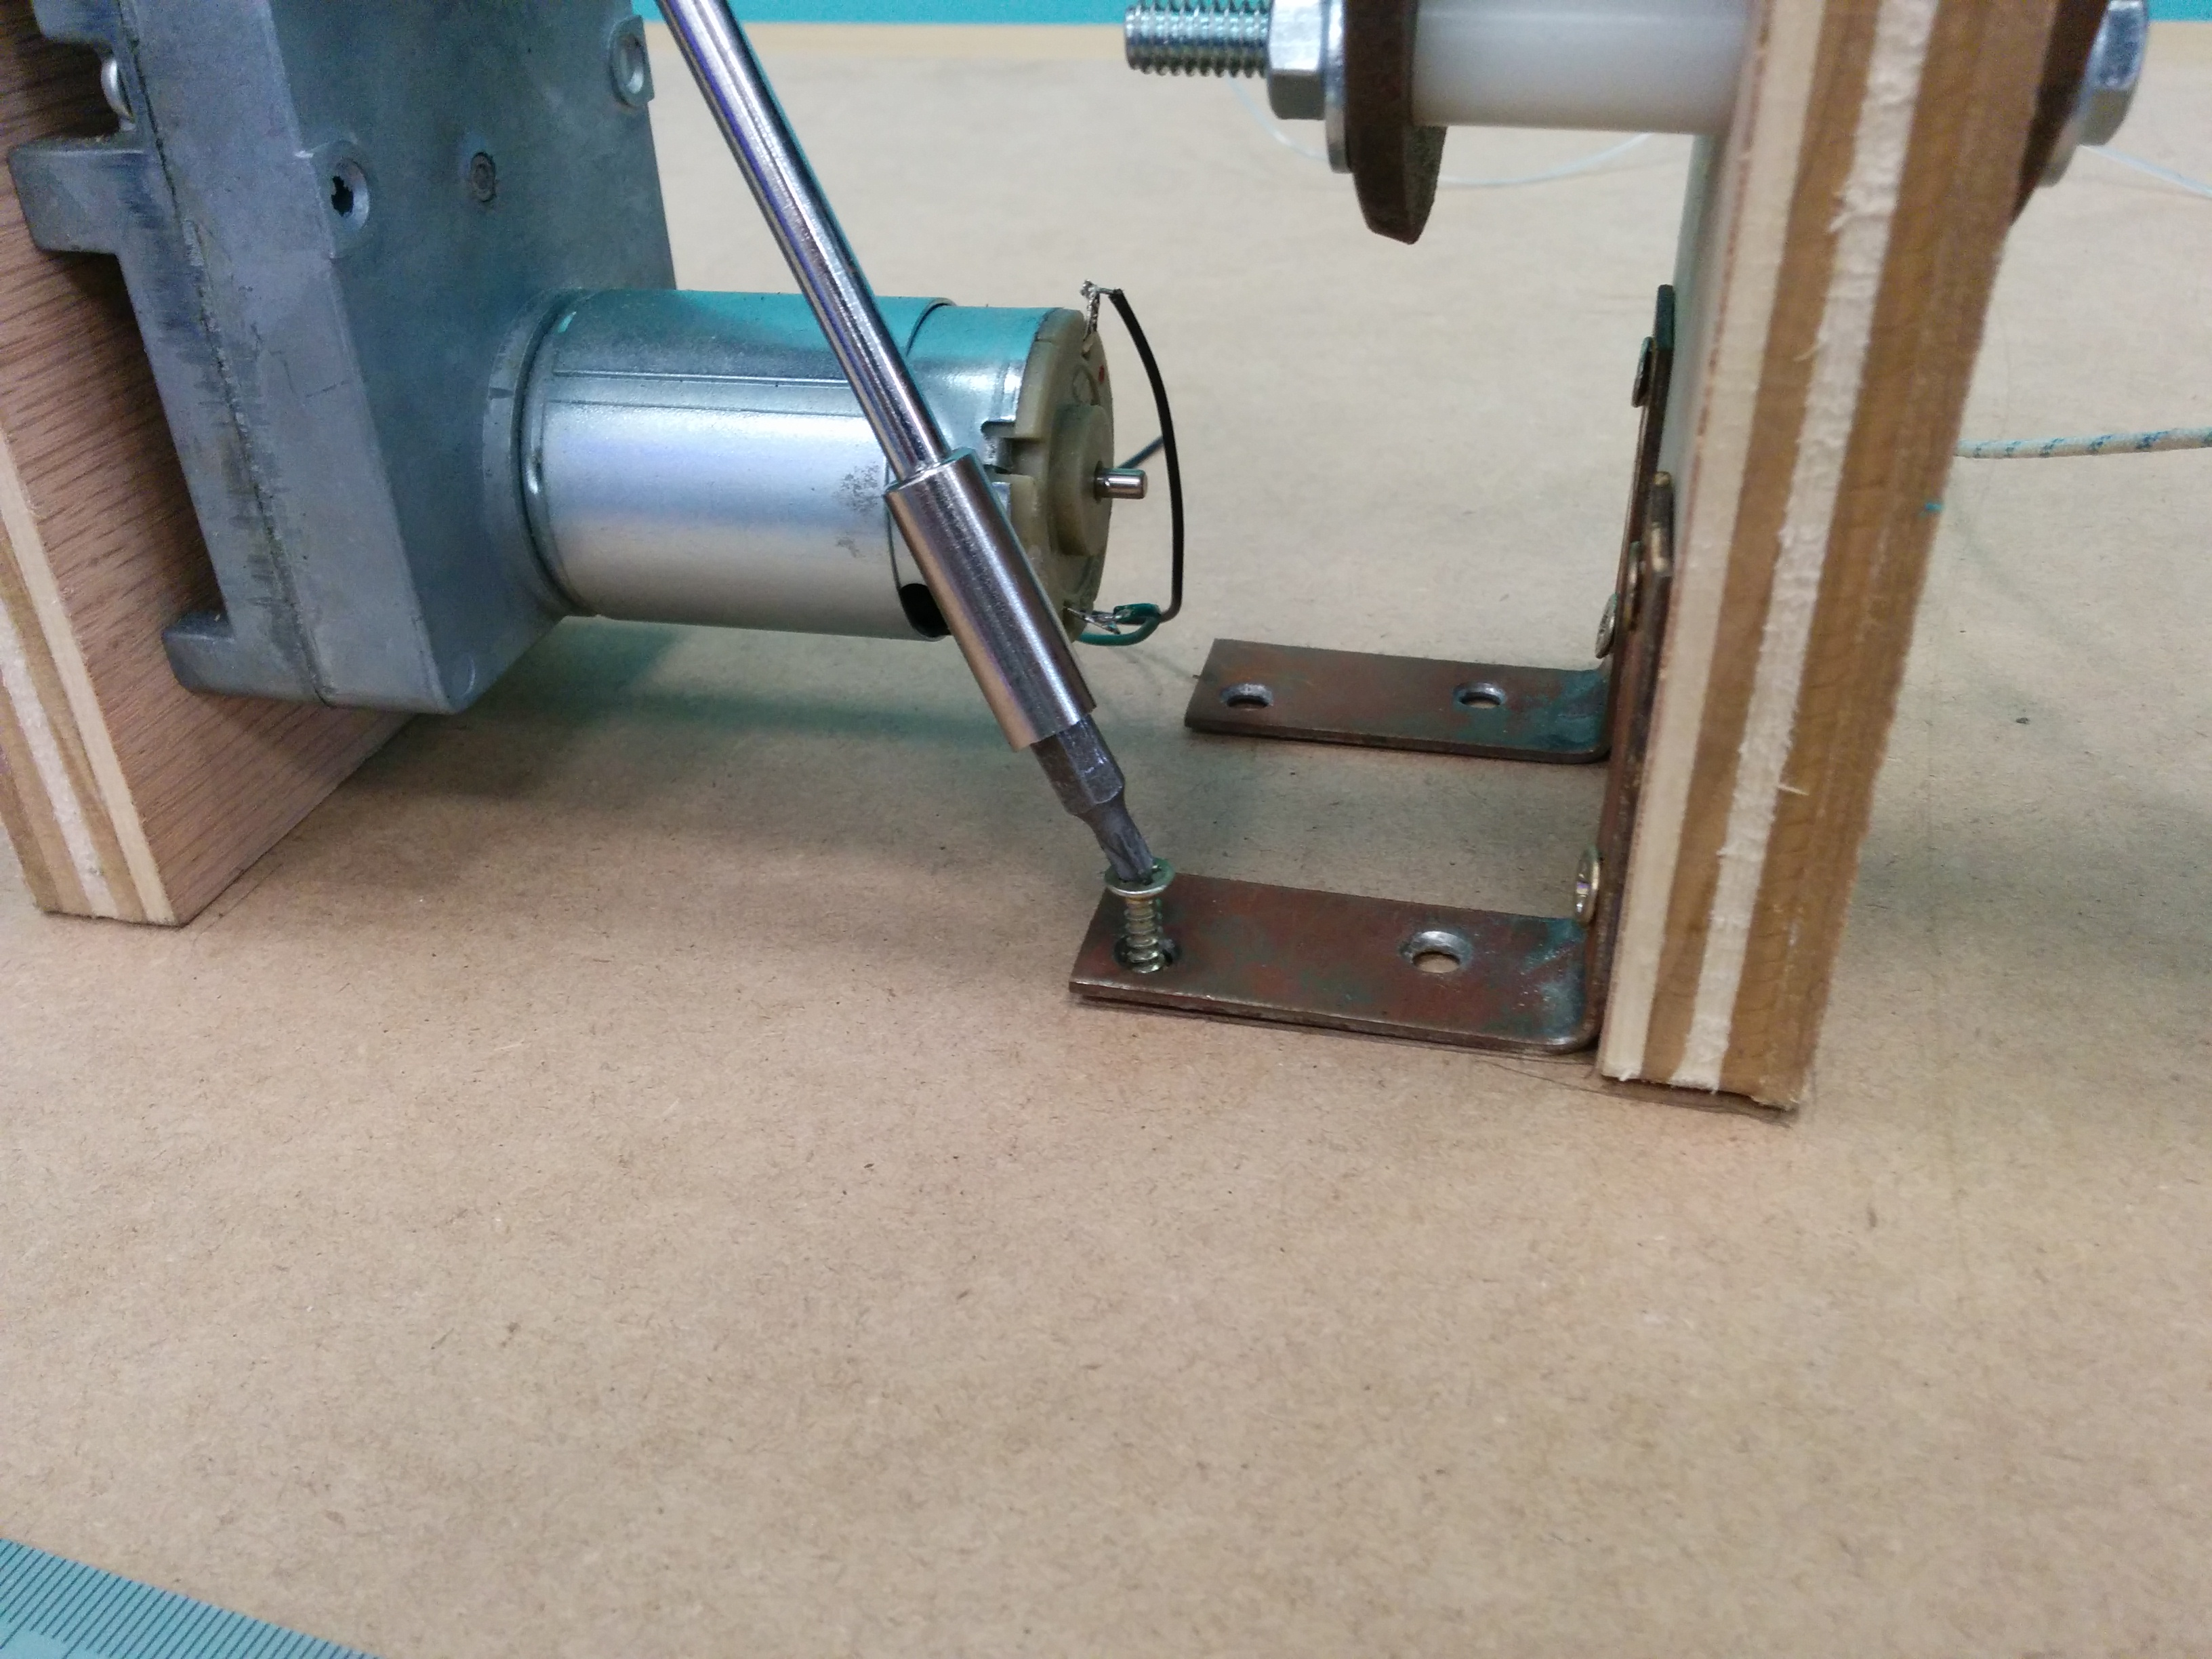
\includegraphics[width=0.6\textwidth]{images/filaextruder/IMG_20150313_114401.jpg}
            \caption{Se ancla la extructura a la base}
            \label{fig:fila_montaje1}
    \end{figure}
    \begin{figure}[H]
            \centering
            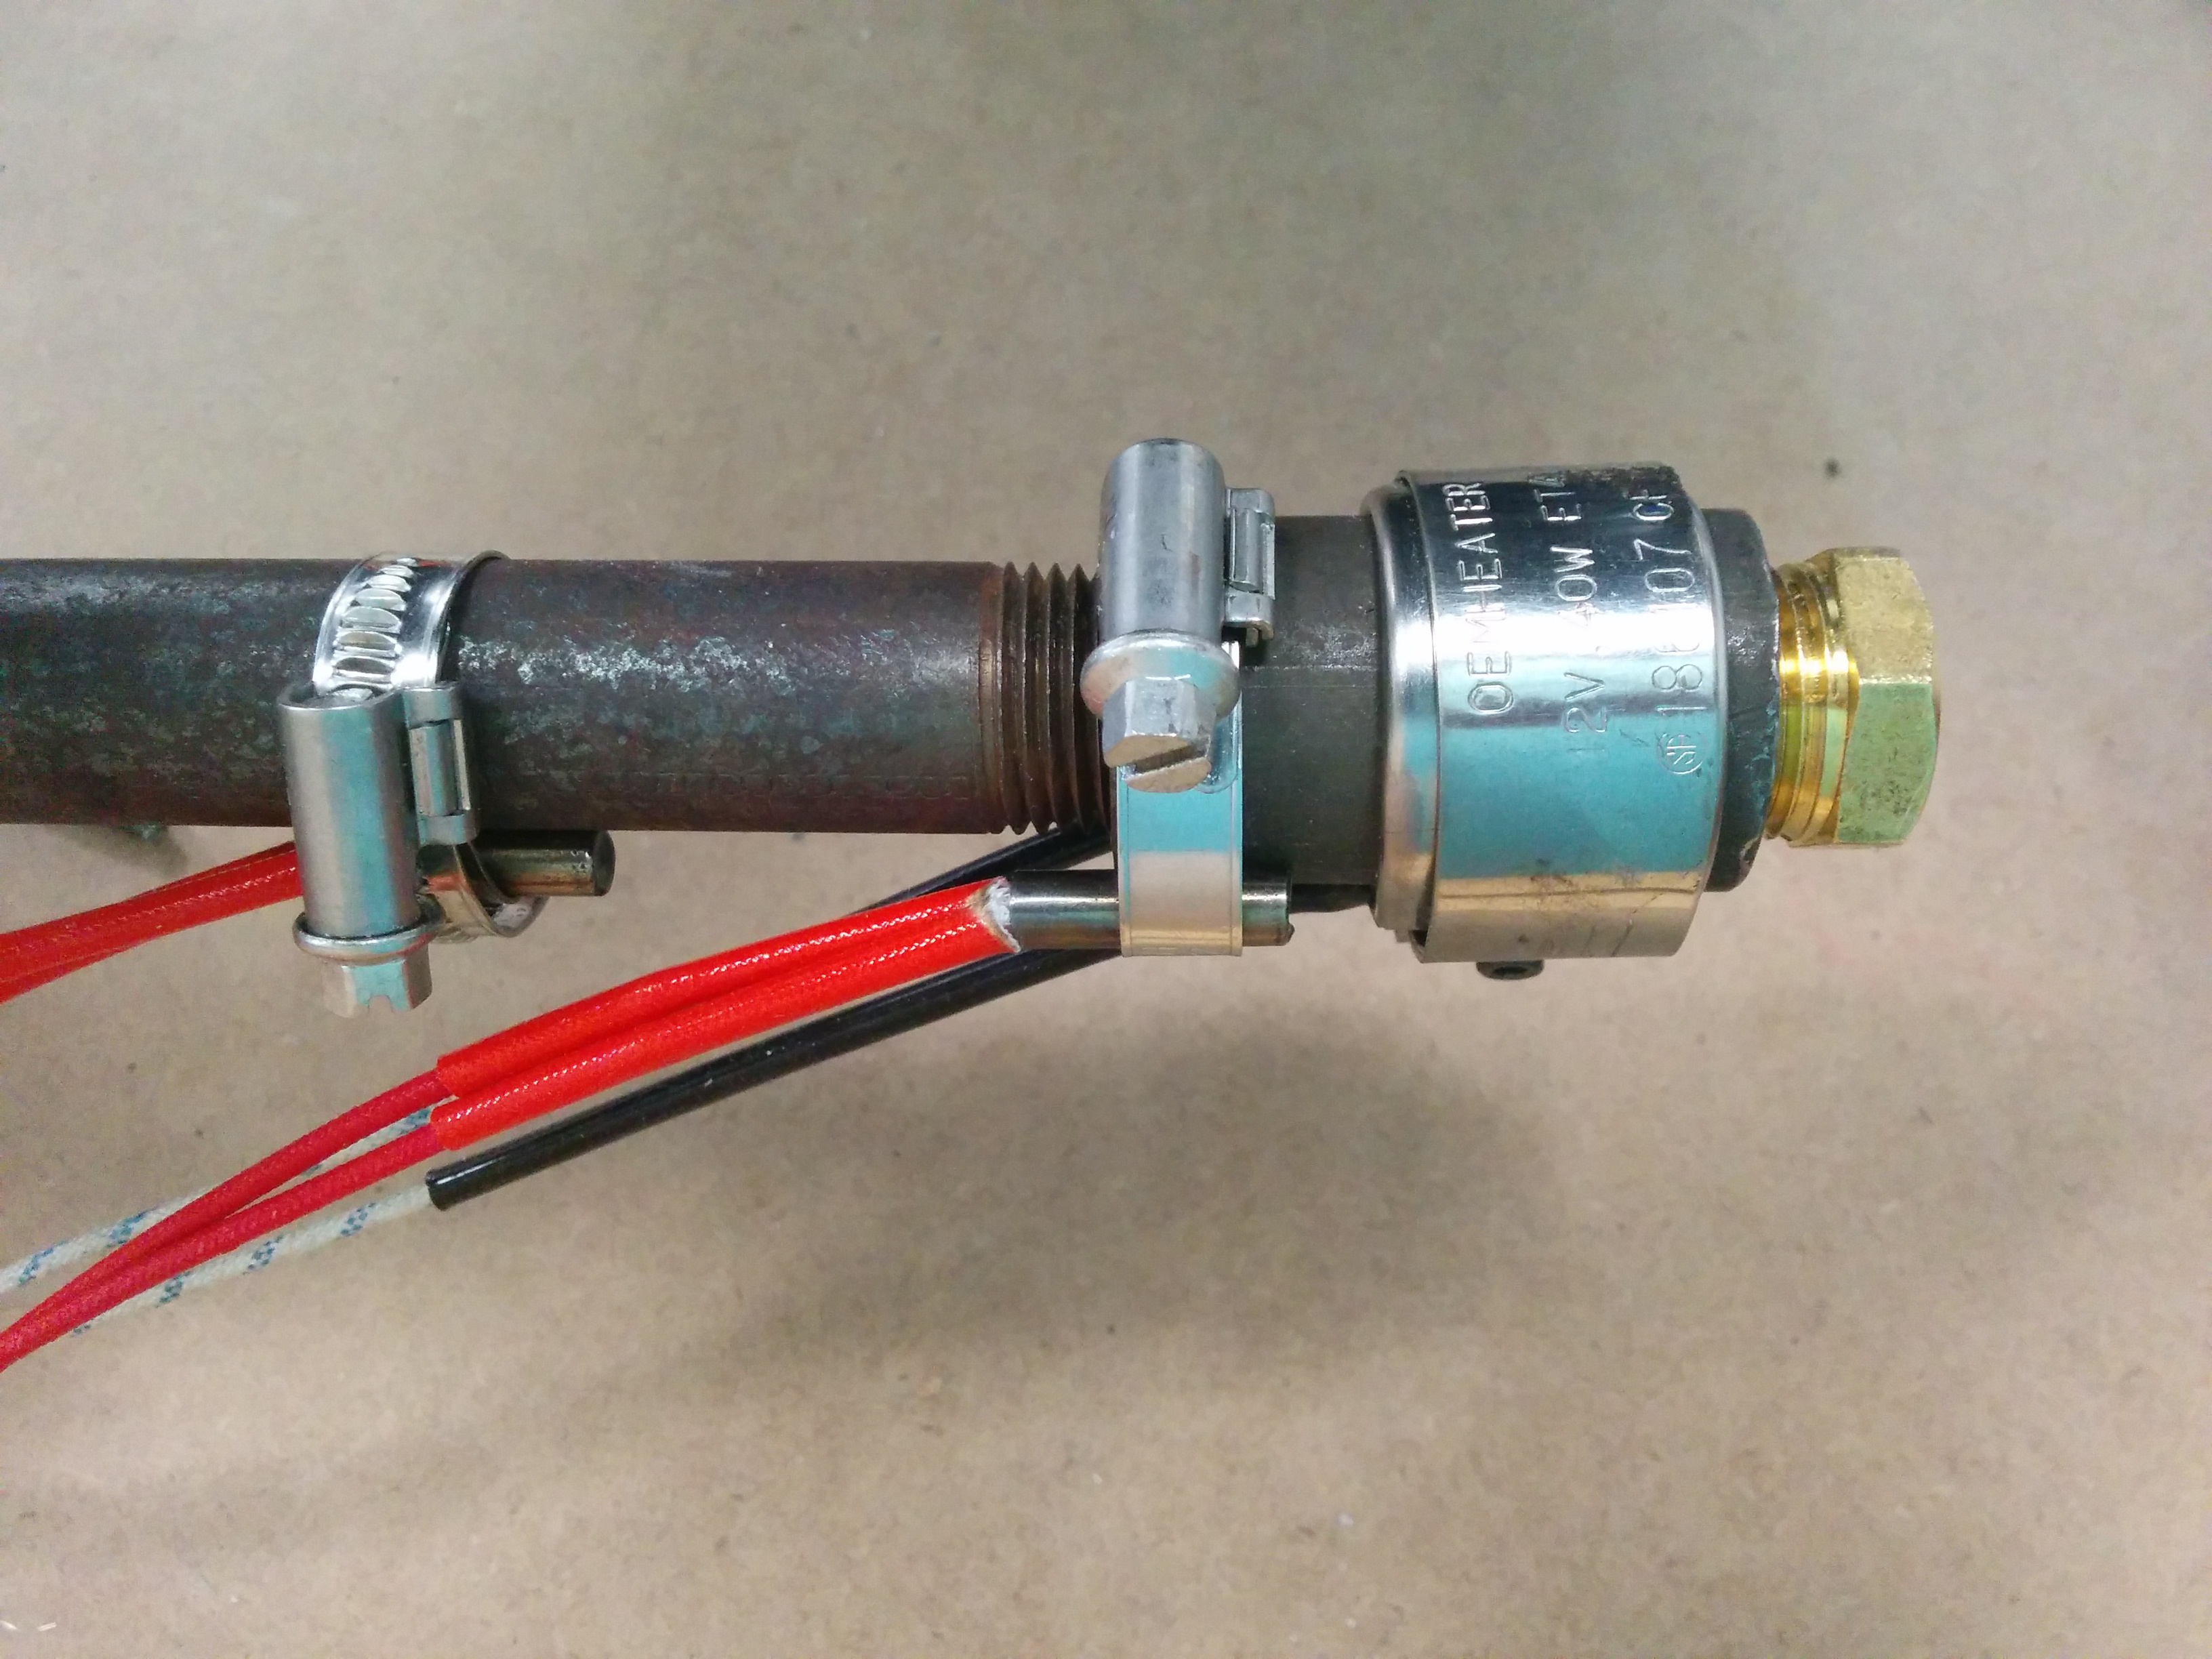
\includegraphics[width=0.6\textwidth]{images/filaextruder/IMG_20150324_175818.jpg}
            \caption{Calefactor en la alimentación y cañon}
            \label{fig:fila_montaje2}
    \end{figure}
    \begin{figure}[H]
            \centering
            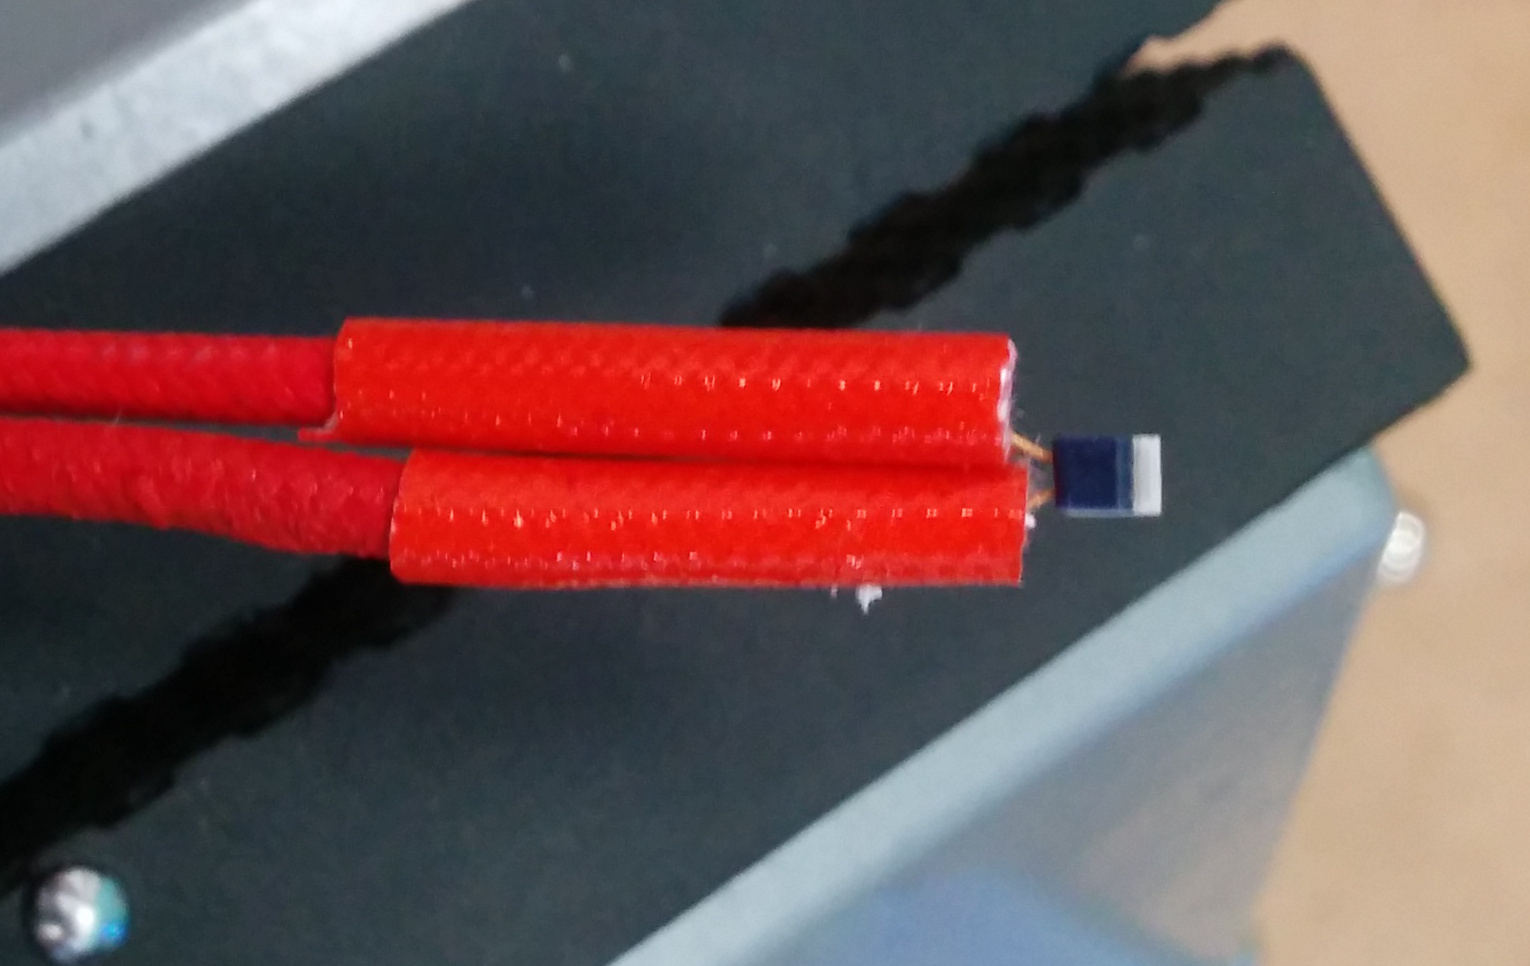
\includegraphics[width=0.6\textwidth]{images/filaextruder/IMG_20150325_145634.jpg}
            \caption{Sensor PT100 de temperatura}
            \label{fig:fila_montaje3}
    \end{figure}

Una vez instalados los cartuchos y las sondas de tempertura en la filastruder, se pasa a aislar el cañon para que la disipación de calor al exterior no sea elevada y poder mantener una temperatura constante.
    \begin{figure}[H]
            \centering
            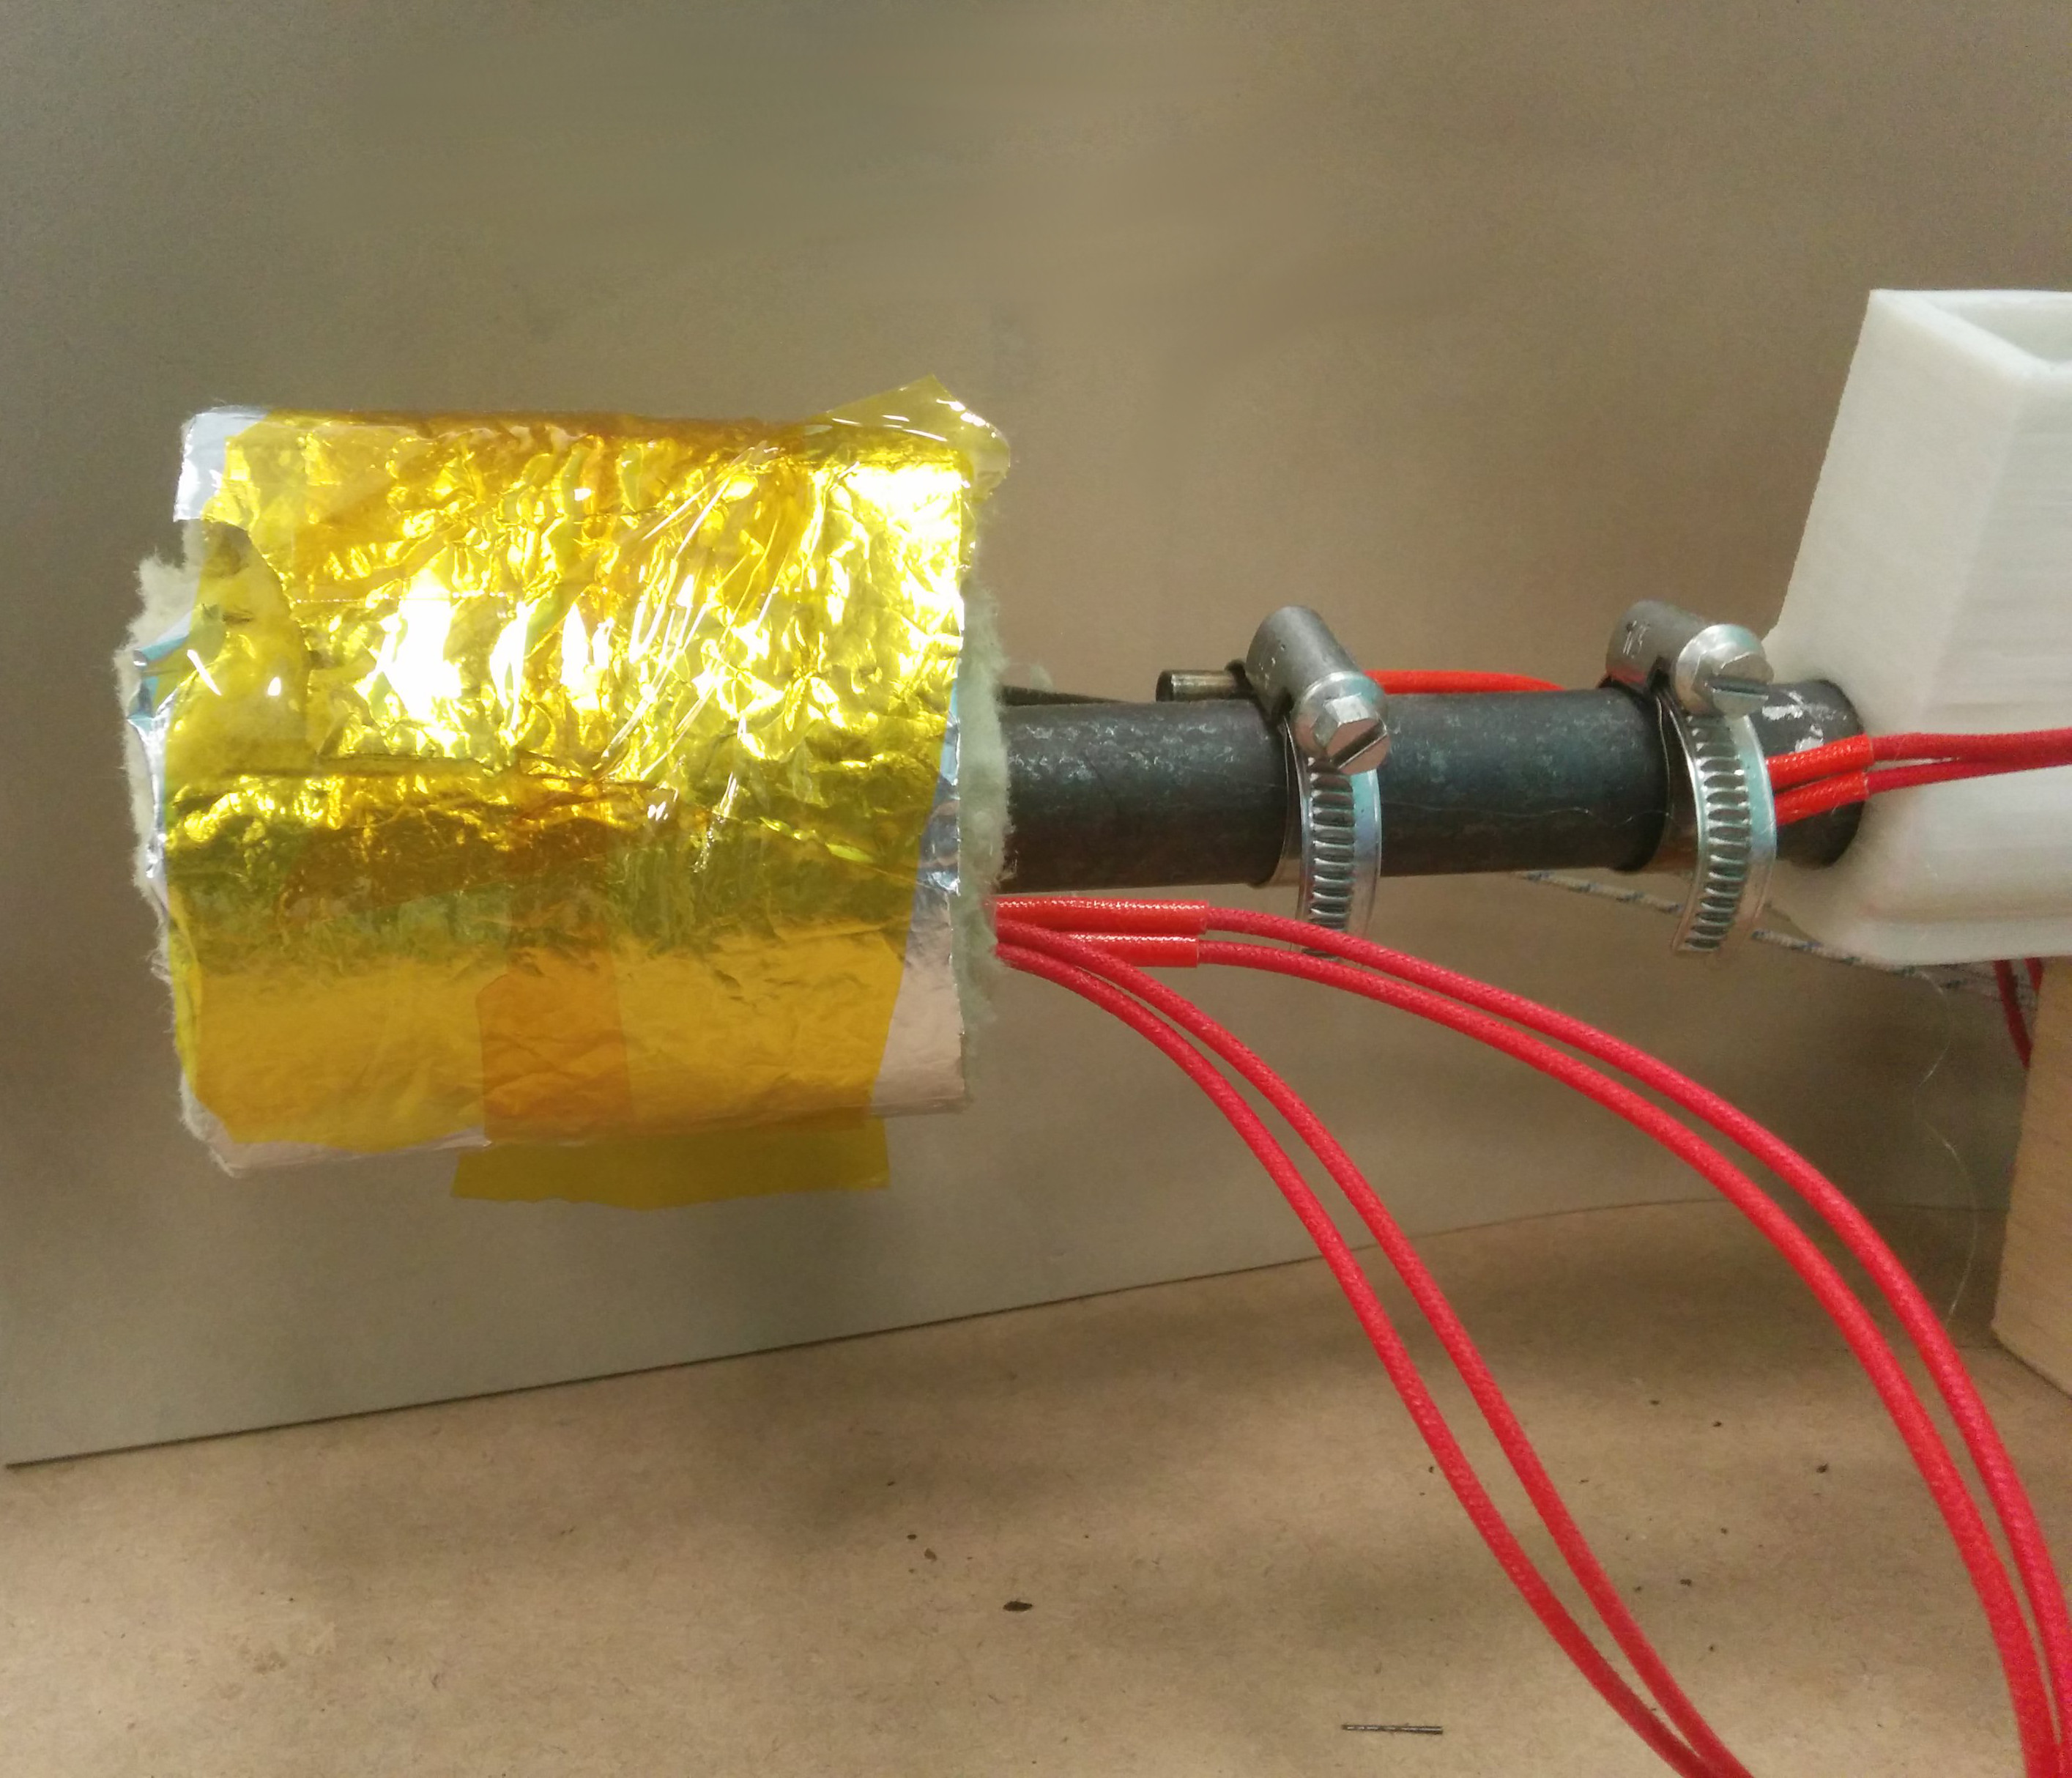
\includegraphics[width=0.4\textwidth]{images/filaextruder/IMG_20150814_132929.jpg}
            \caption{Filastruder montado}
            \label{fig:fila_montaje4}
    \end{figure}

El siguiente paso es cablear todas las señales a un armario que instalaremos en la propia maqueta en el espacio reservado para ello, este armario estará conectado al armario del PLC para poder realizar el control de la maqueta:

\begin{itemize}
	\item Sondas de temperatura.
	\item Reles para controlar las resistencias de potencia y el motor del husillo.
\end{itemize}


El circuito eléctrico a cablear está indicado en el Anexo \ref{ane:esquemas_electricos}.
    \begin{figure}[H]
            \centering
            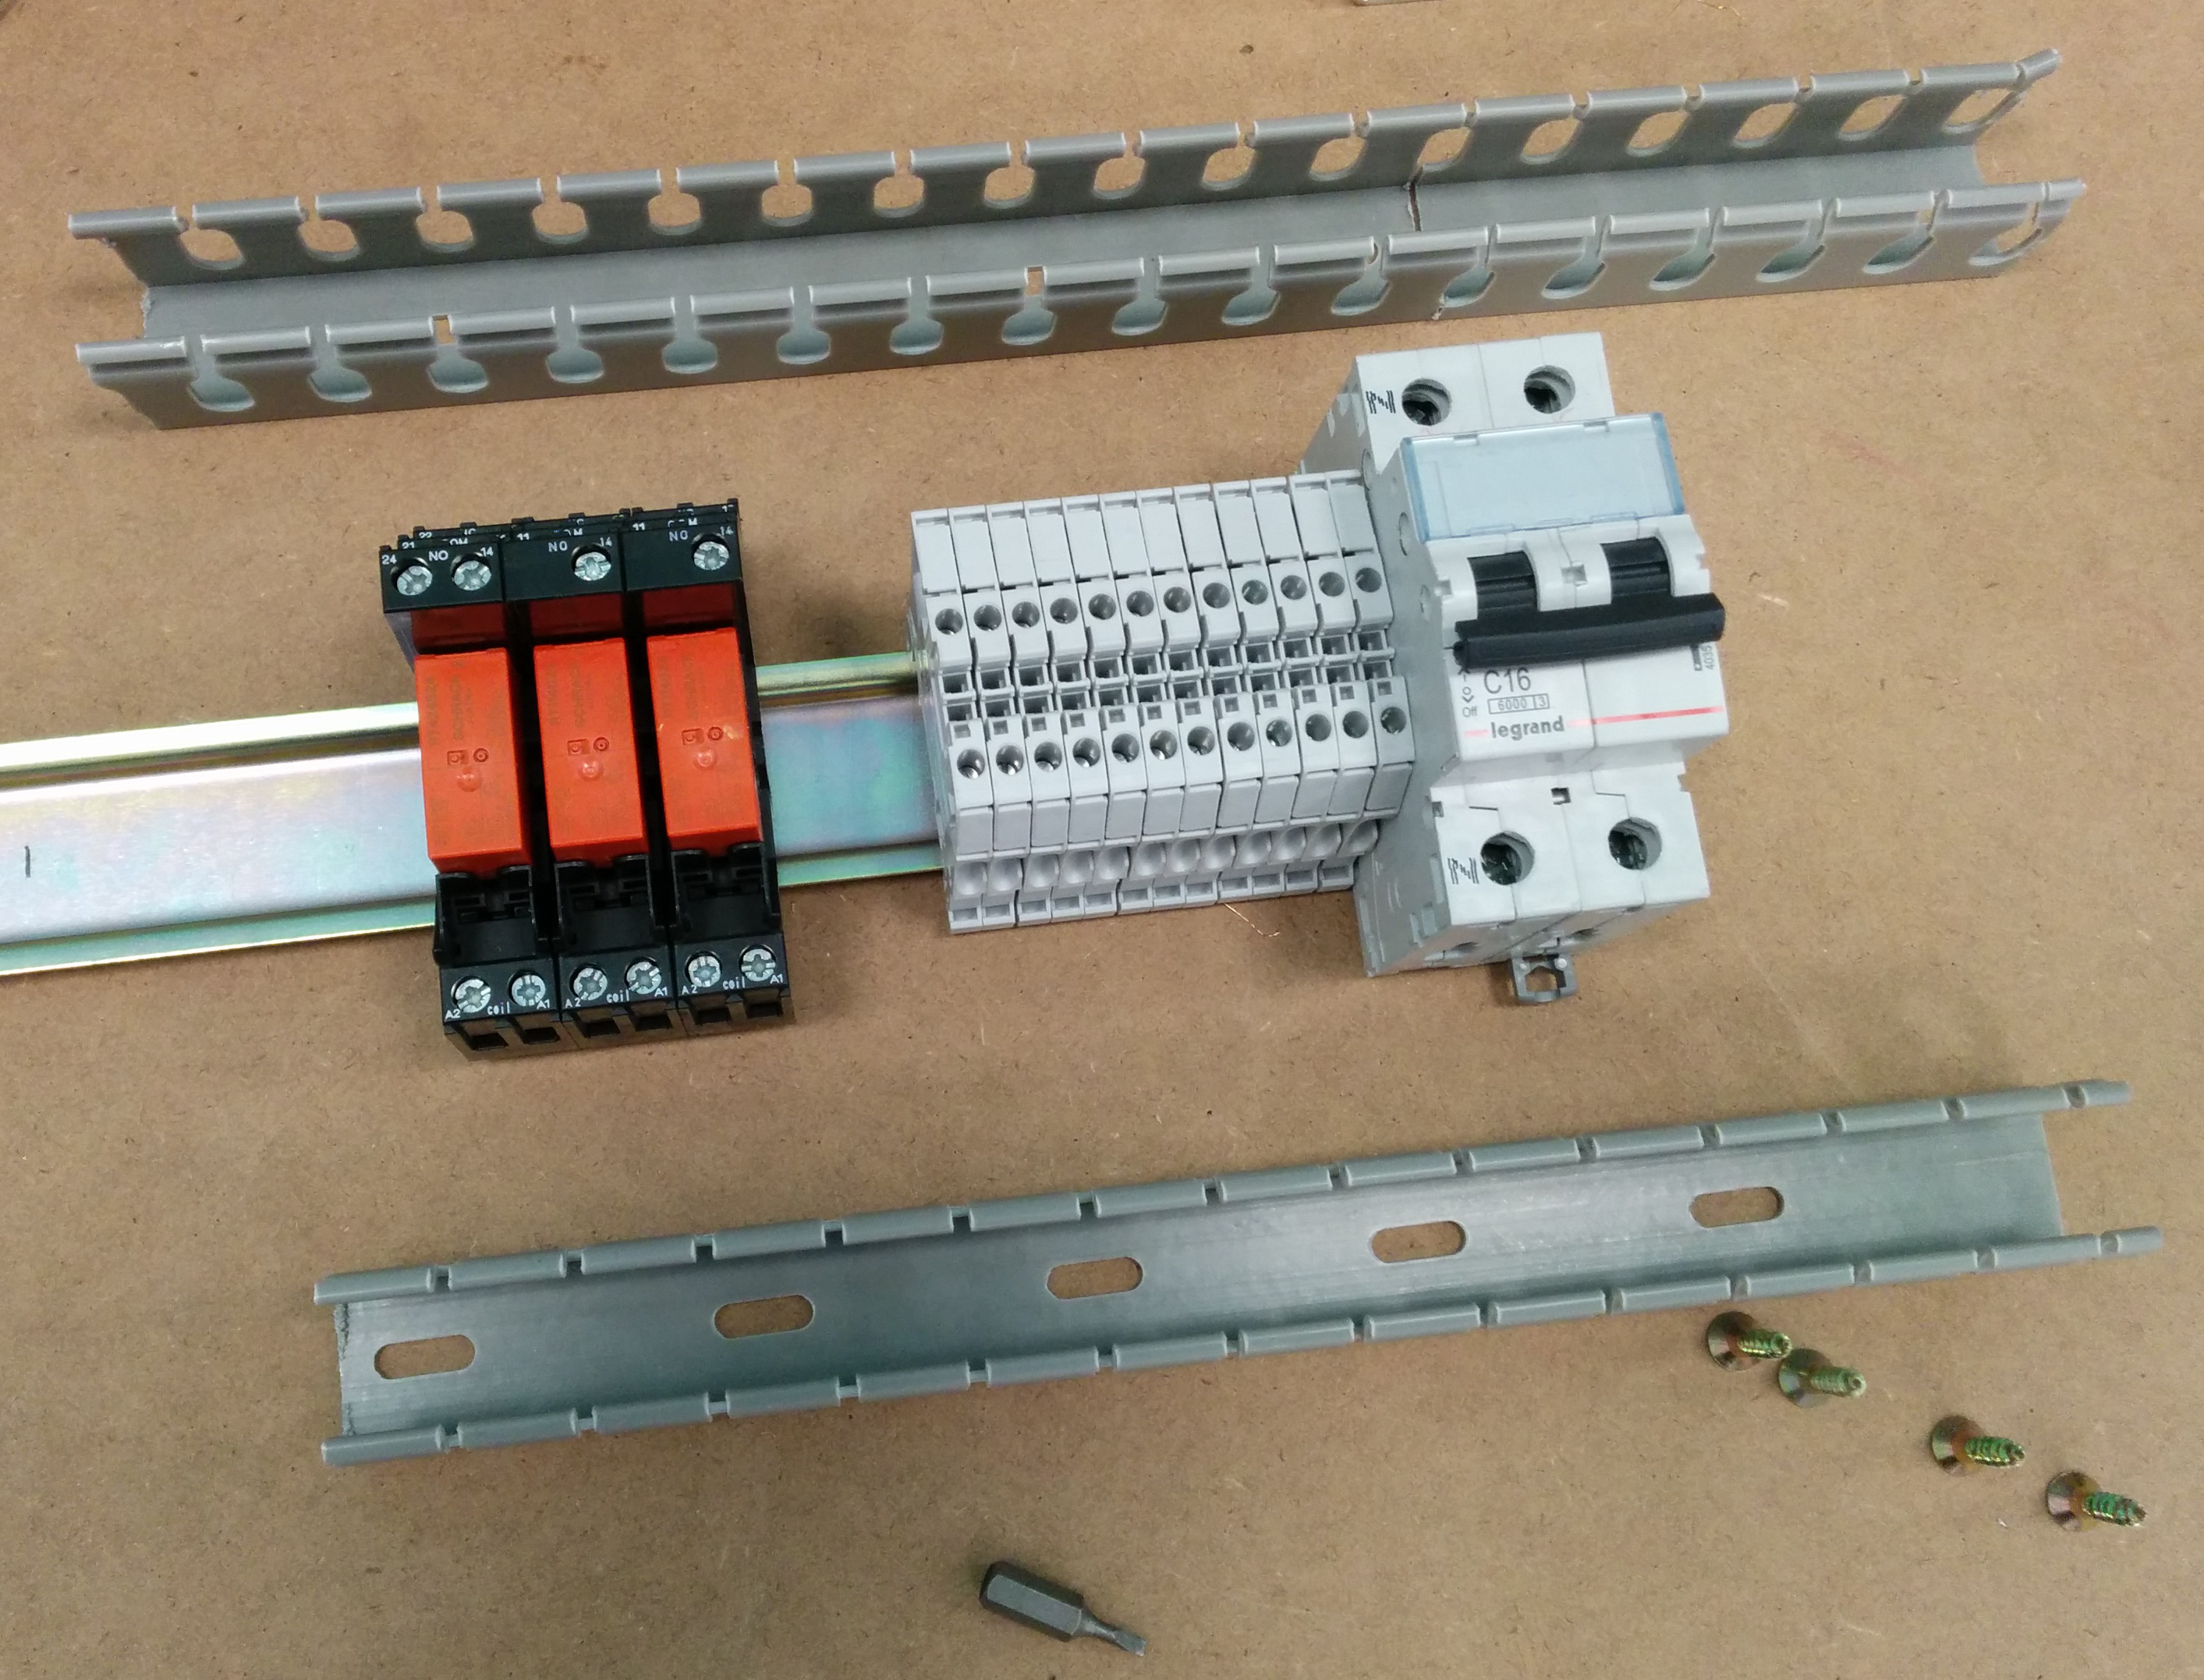
\includegraphics[width=0.5\textwidth]{images/maqueta/IMG_20150324_162200.jpg}
            \caption{Presentación de los componentes en el lugar adecuado.}
            \label{fig:maque_montaje5}
    \end{figure}
    \begin{figure}[H]
            \centering
            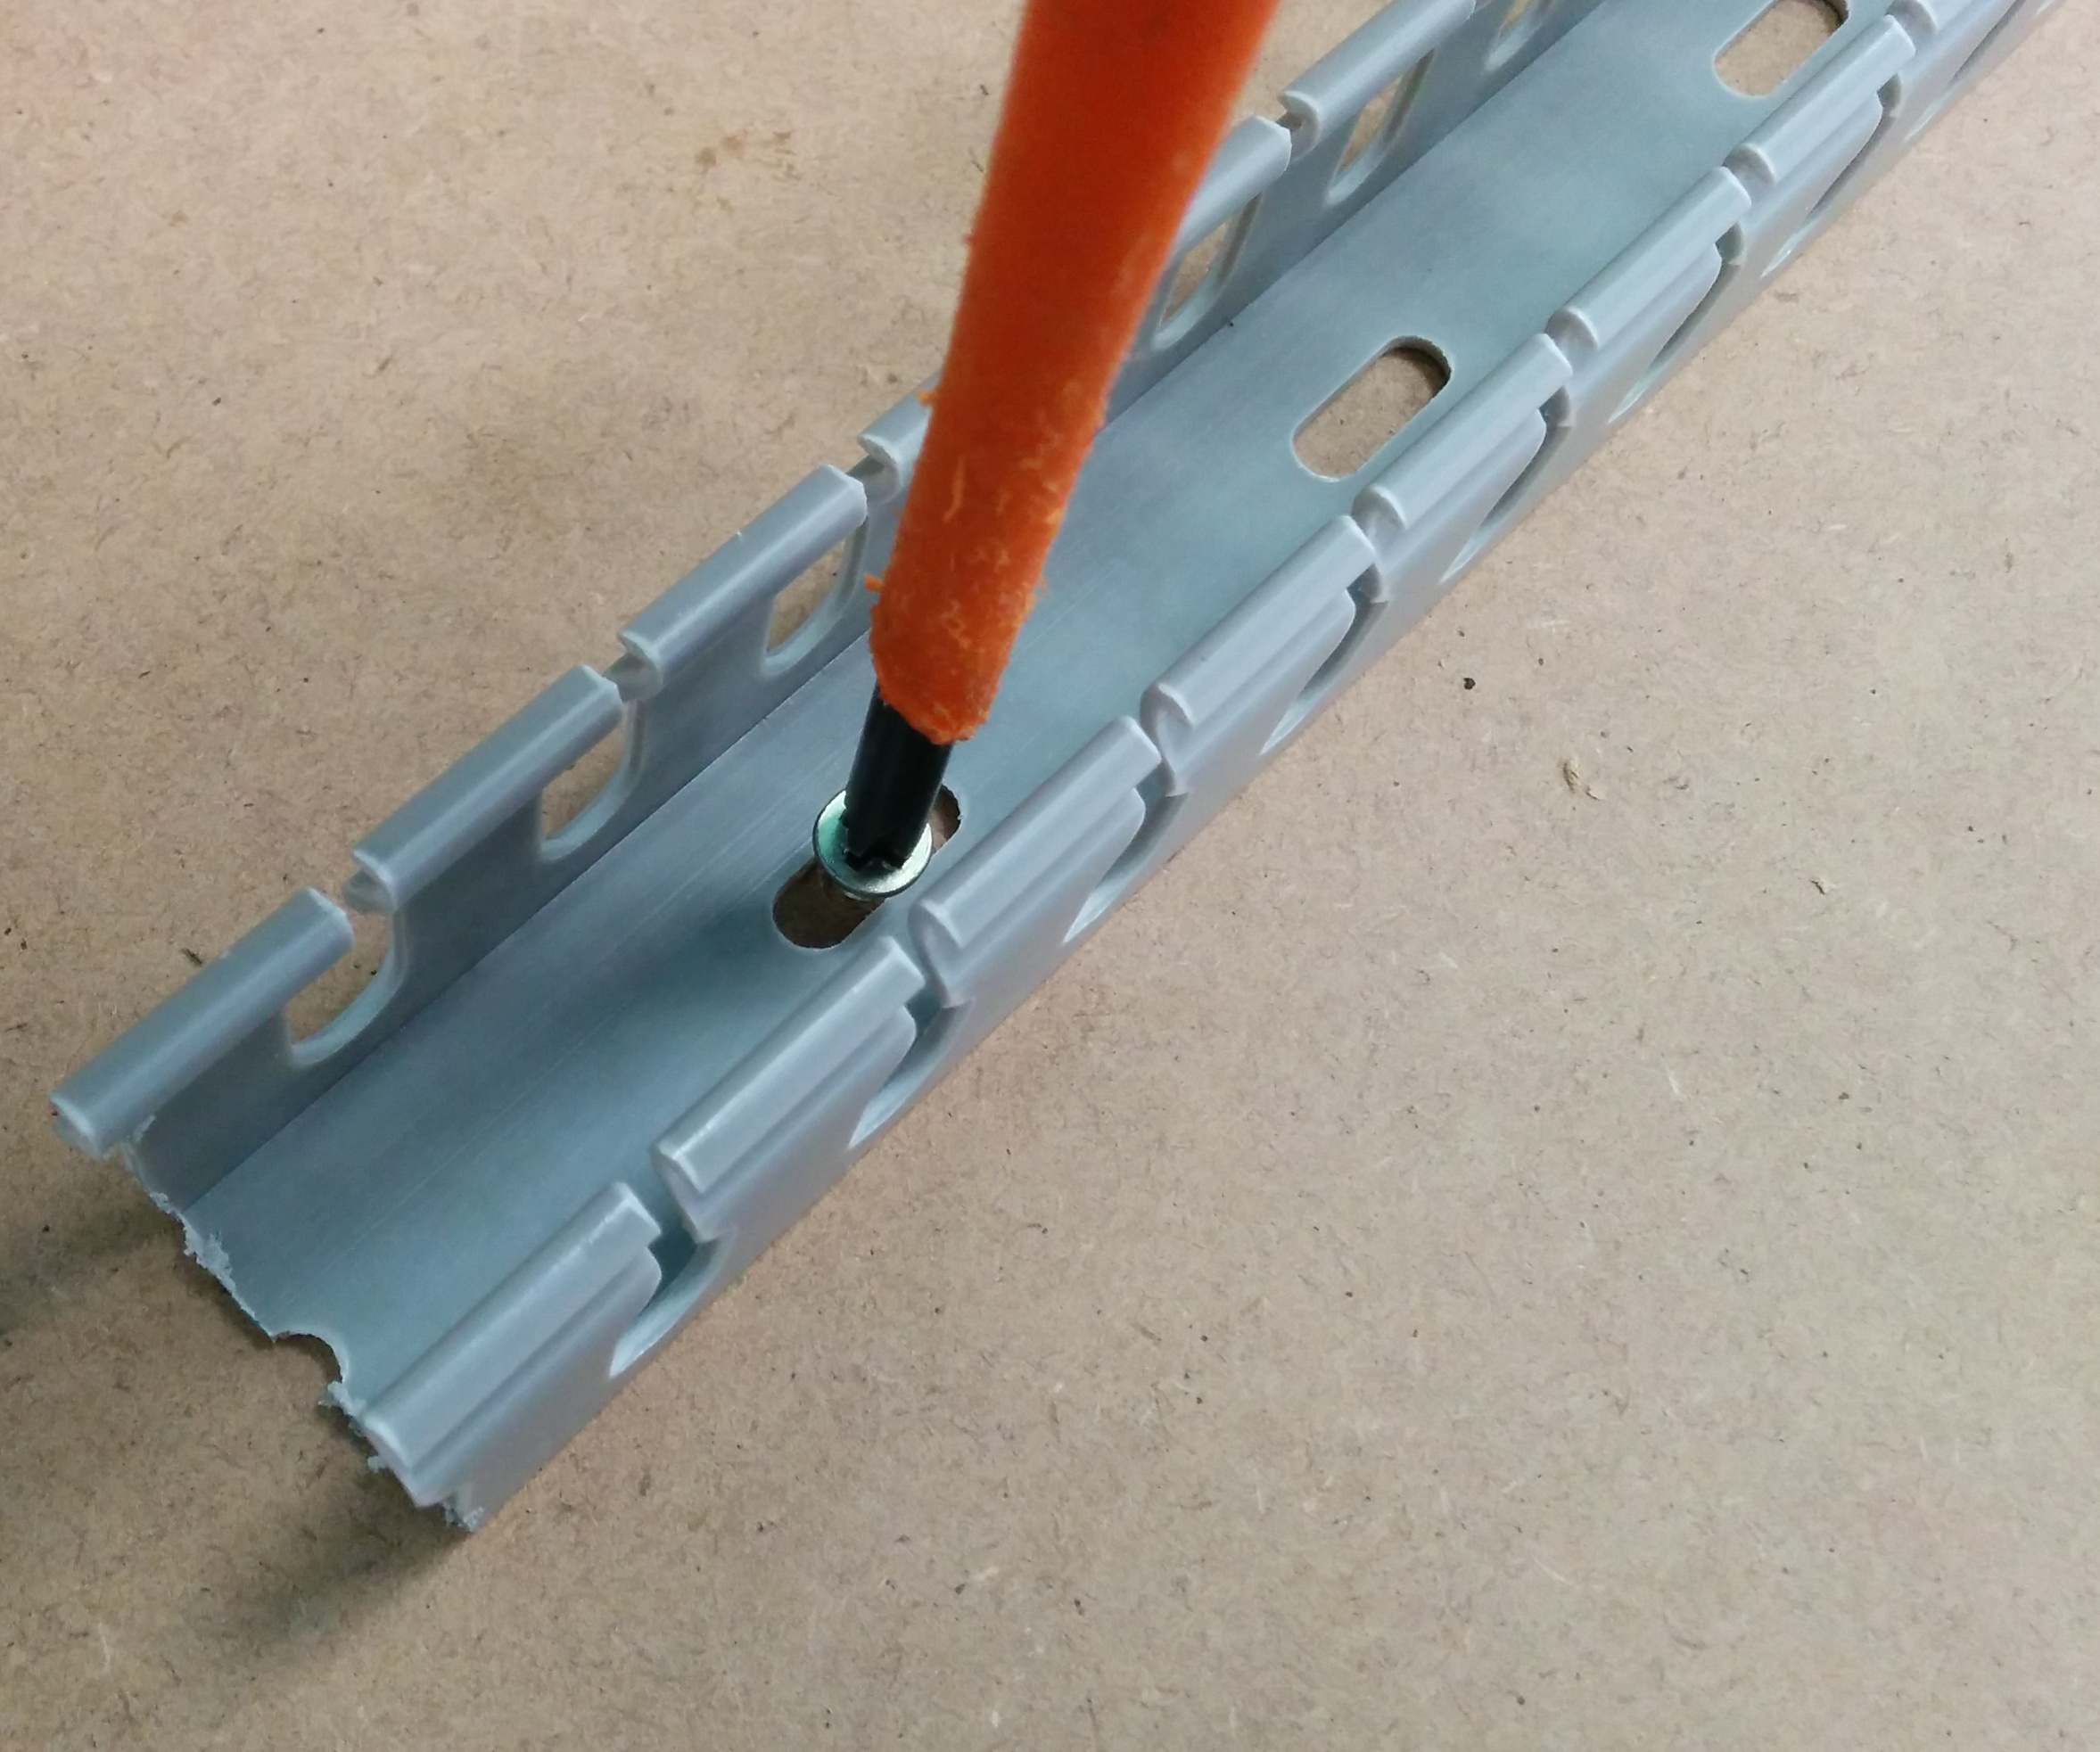
\includegraphics[width=0.5\textwidth]{images/maqueta/IMG_20150324_162705.jpg}
            \caption{Atornillamos las canaletas y guias a la madera.}
            \label{fig:maque_montaje6}
    \end{figure}
    \begin{figure}[H]
            \centering
            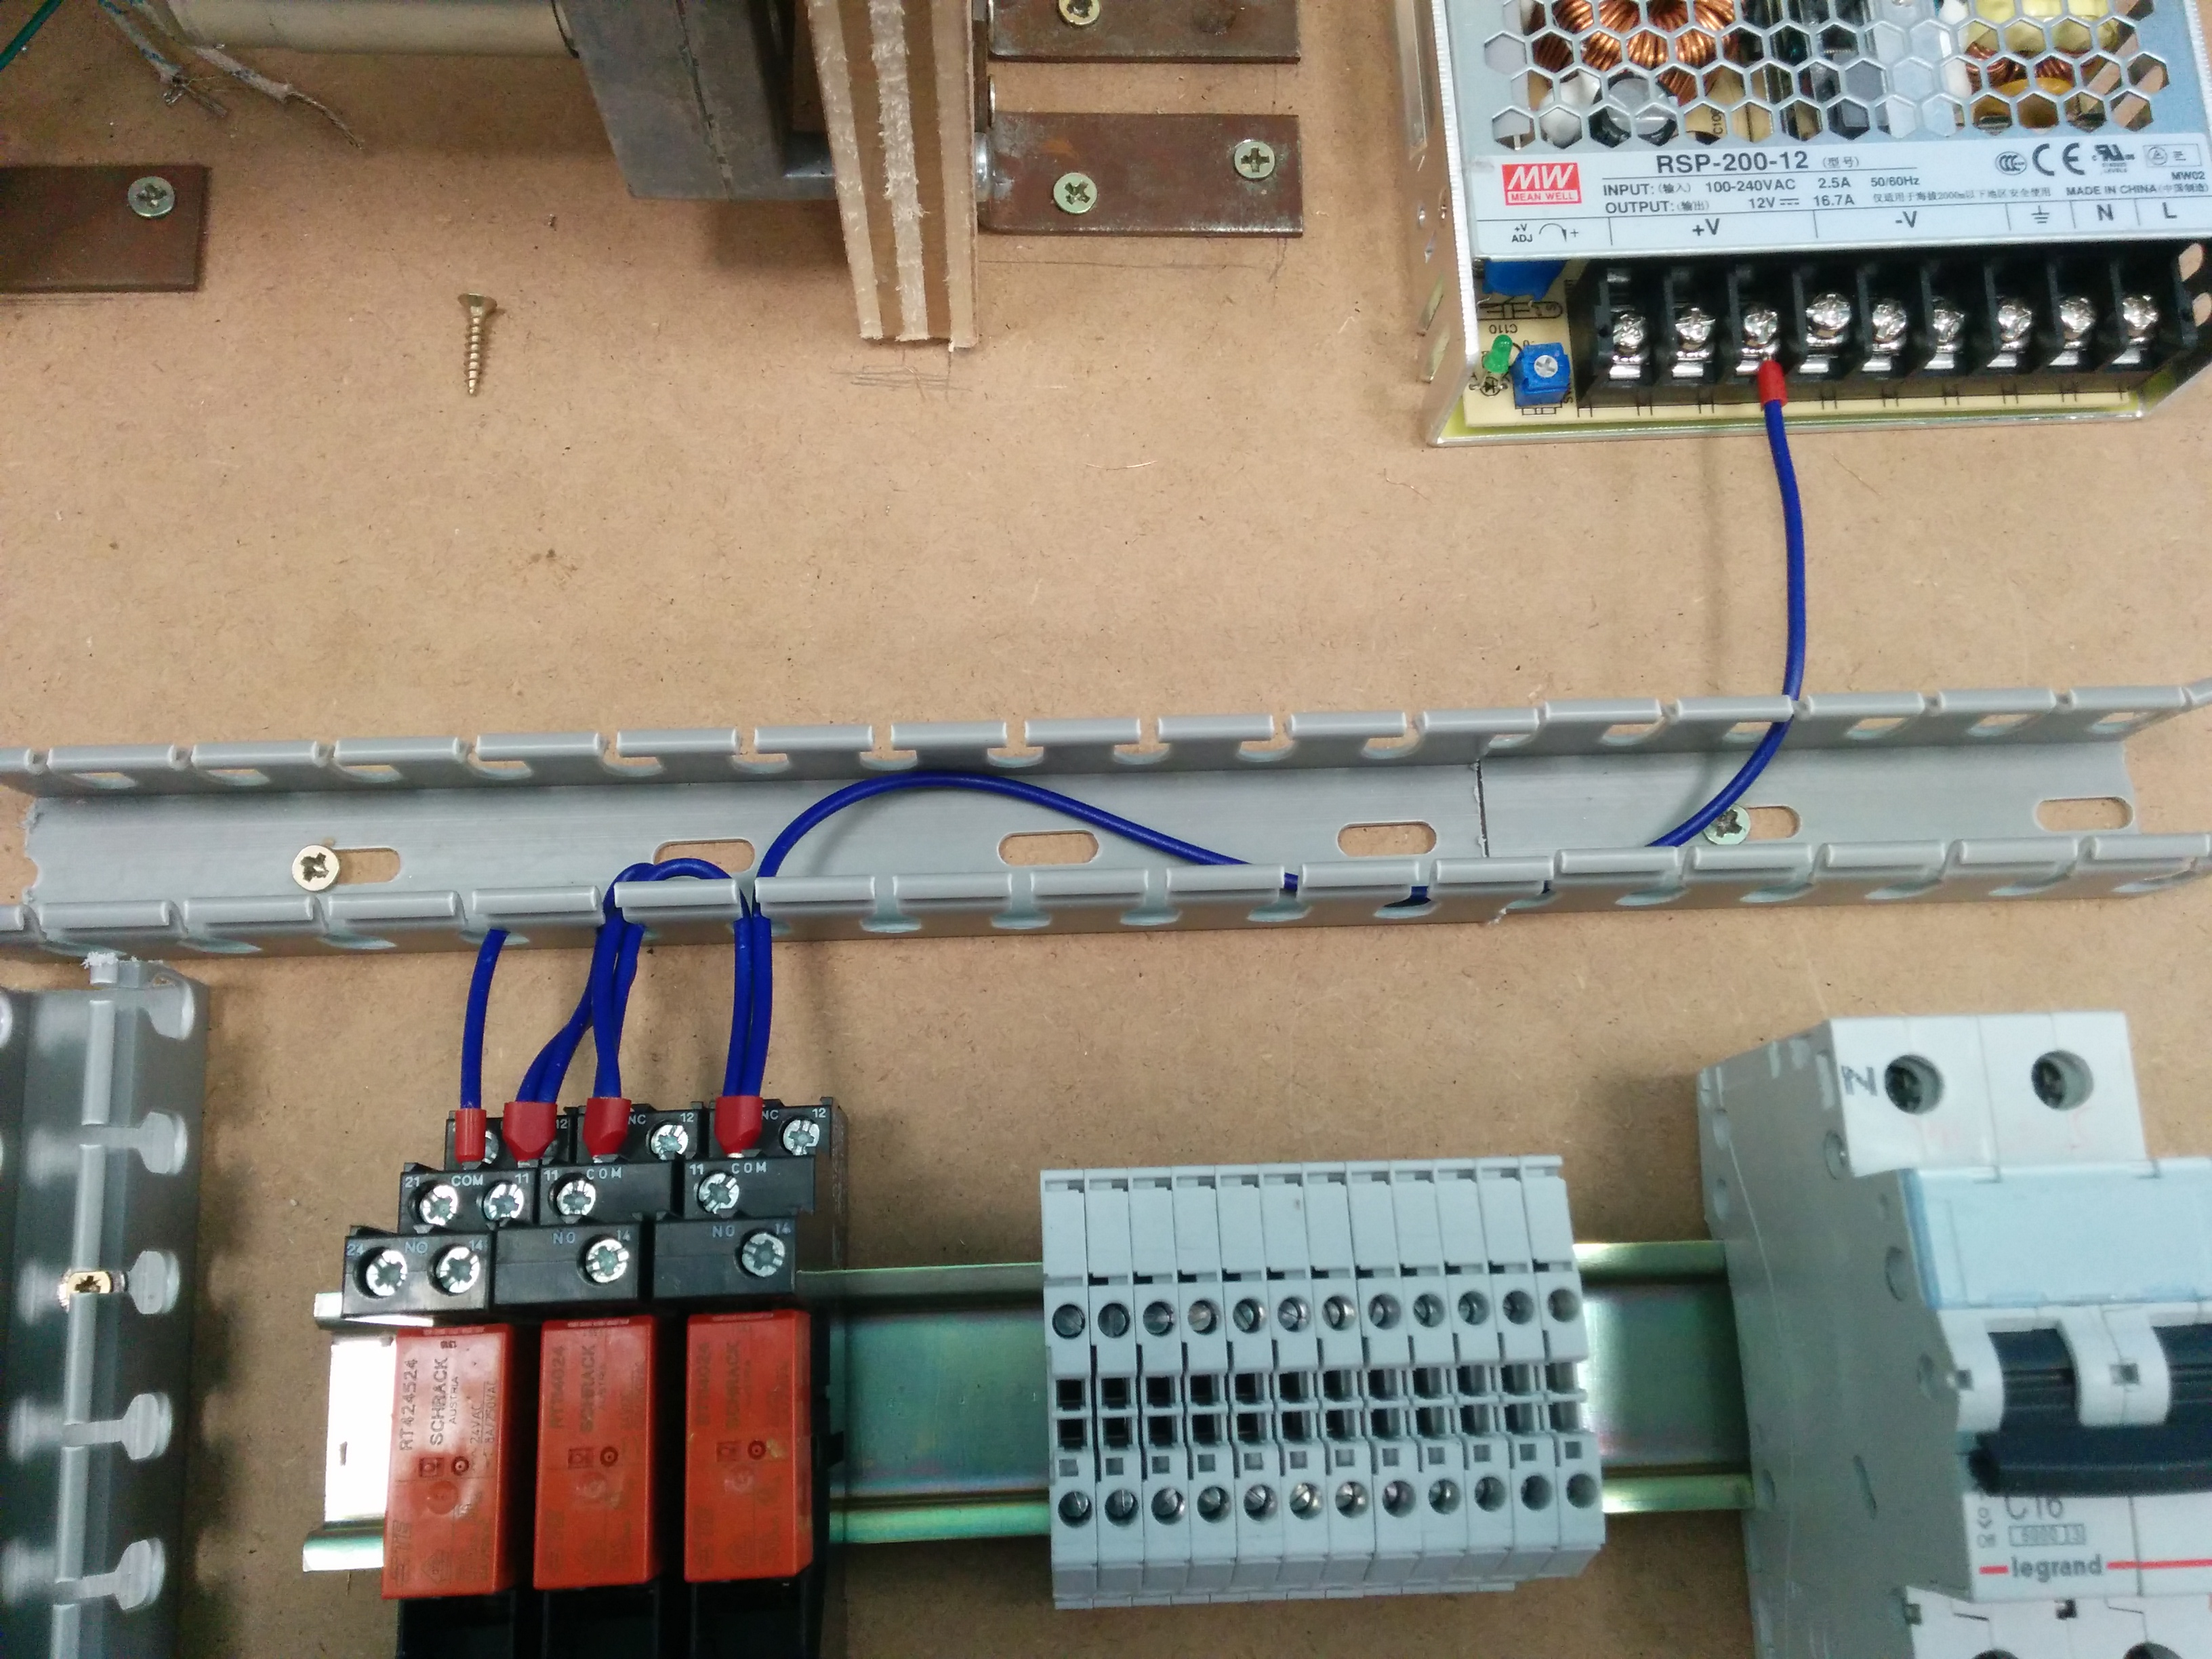
\includegraphics[width=0.5\textwidth]{images/maqueta/IMG_20150324_173716.jpg}
            \caption{Cableamos los componentes según los esquemas.}
            \label{fig:maque_montaje7}
    \end{figure}
    \begin{figure}[H]
            \centering
            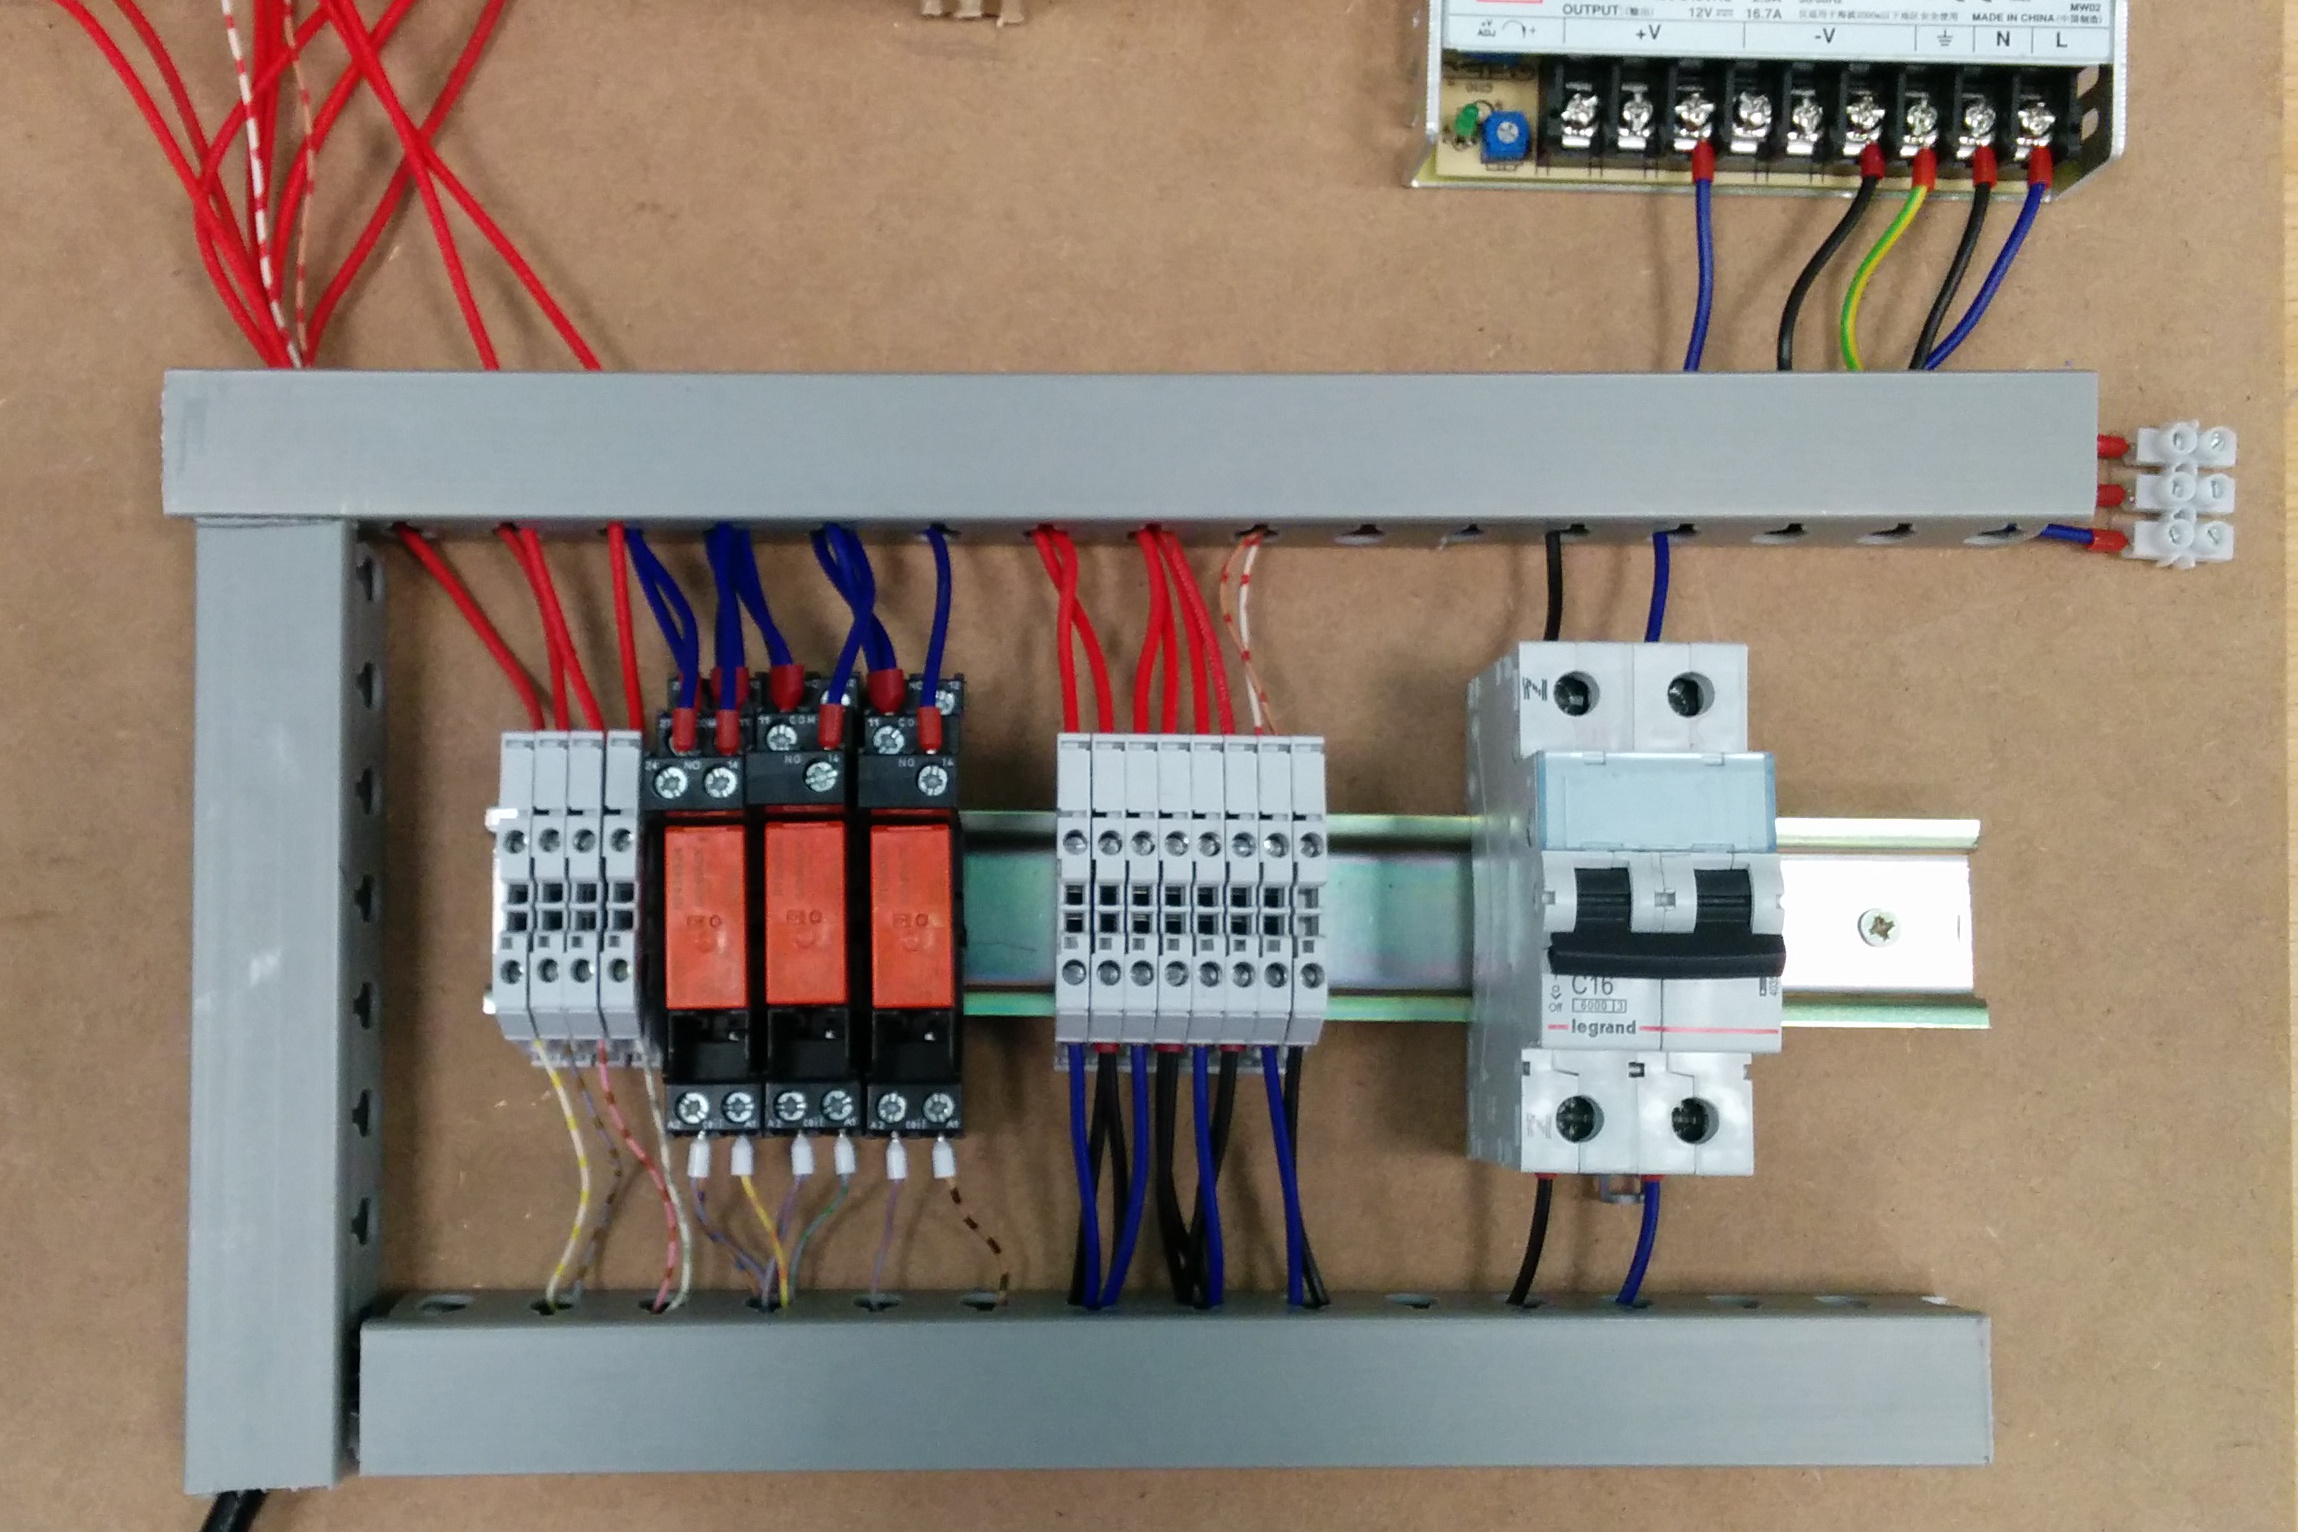
\includegraphics[width=0.5\textwidth]{images/maqueta/IMG_20150331_125243.jpg}
            \caption{Aspecto final cuadro eléctrico maqueta.}
            \label{fig:maque_montaje8}
    \end{figure}

A continuación se va a realizar el montaje del armario eléctrico

    \begin{figure}[H]
            \centering
            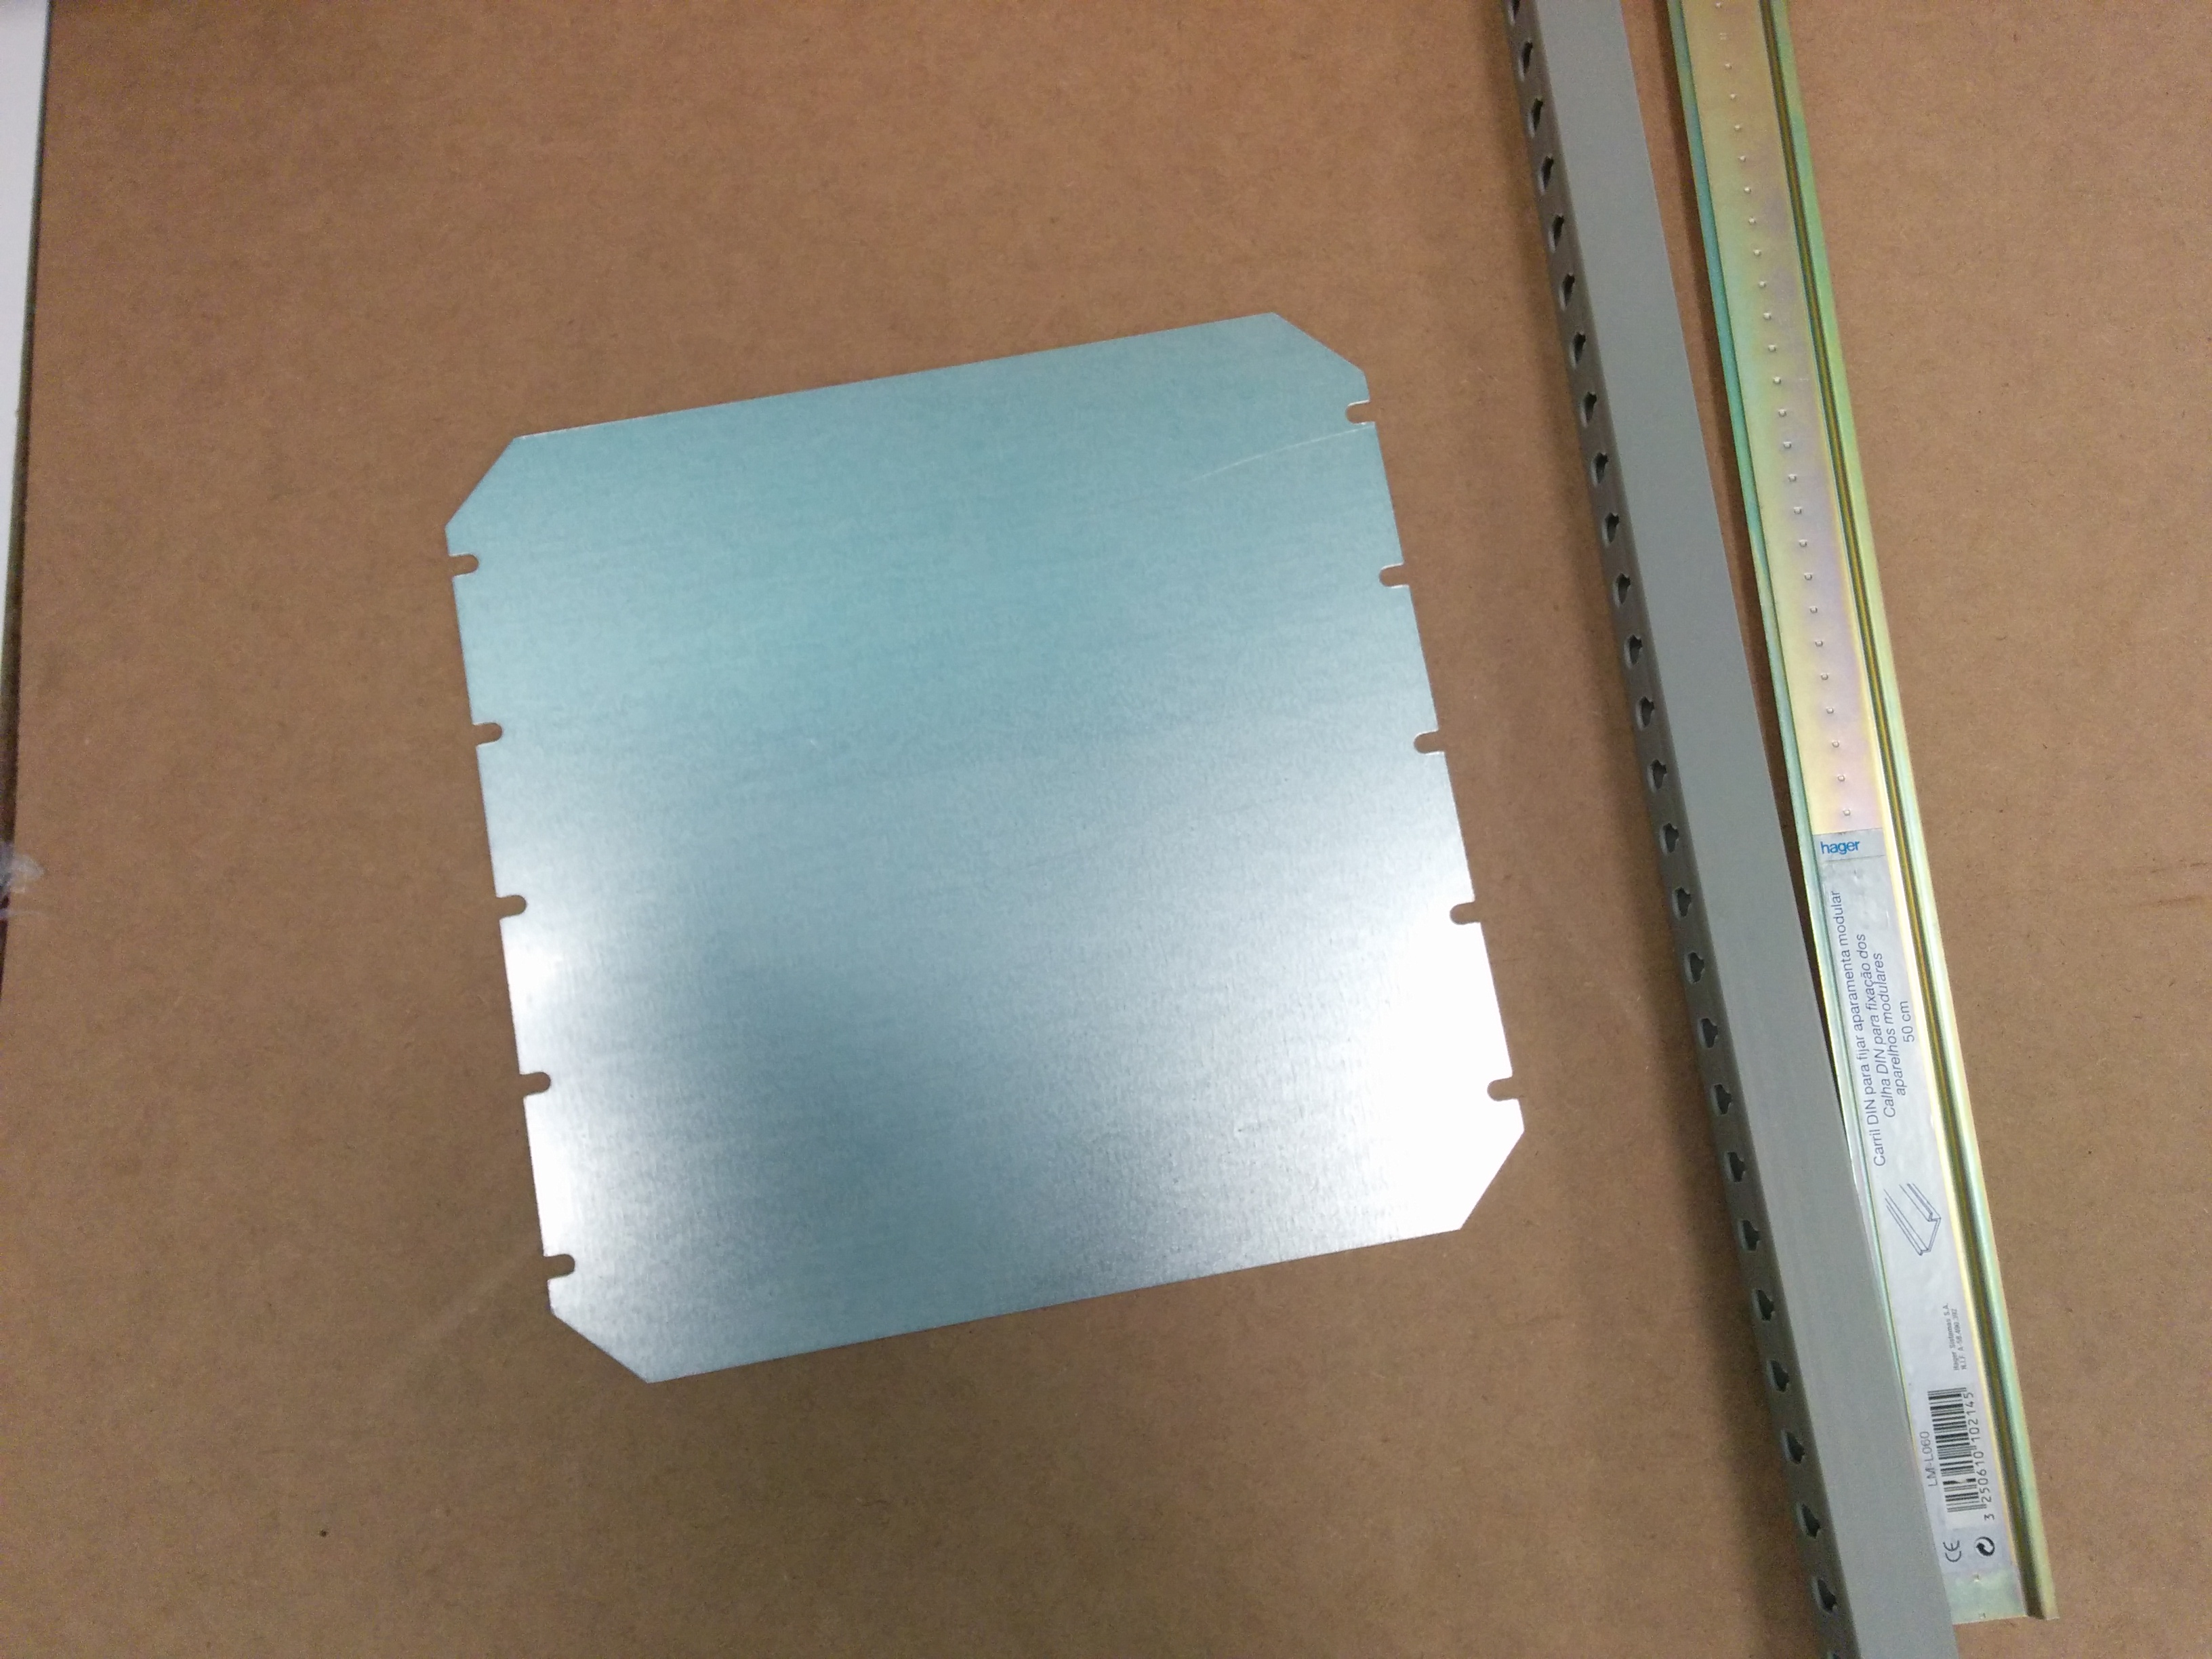
\includegraphics[width=0.5\textwidth]{images/cuadro/IMG_20150311_162414.jpg}
            \caption{Lámina, canaleta y guía donde irá el PLC.}
            \label{fig:cuad_montaje1}
    \end{figure}
    \begin{figure}[H]
            \centering
            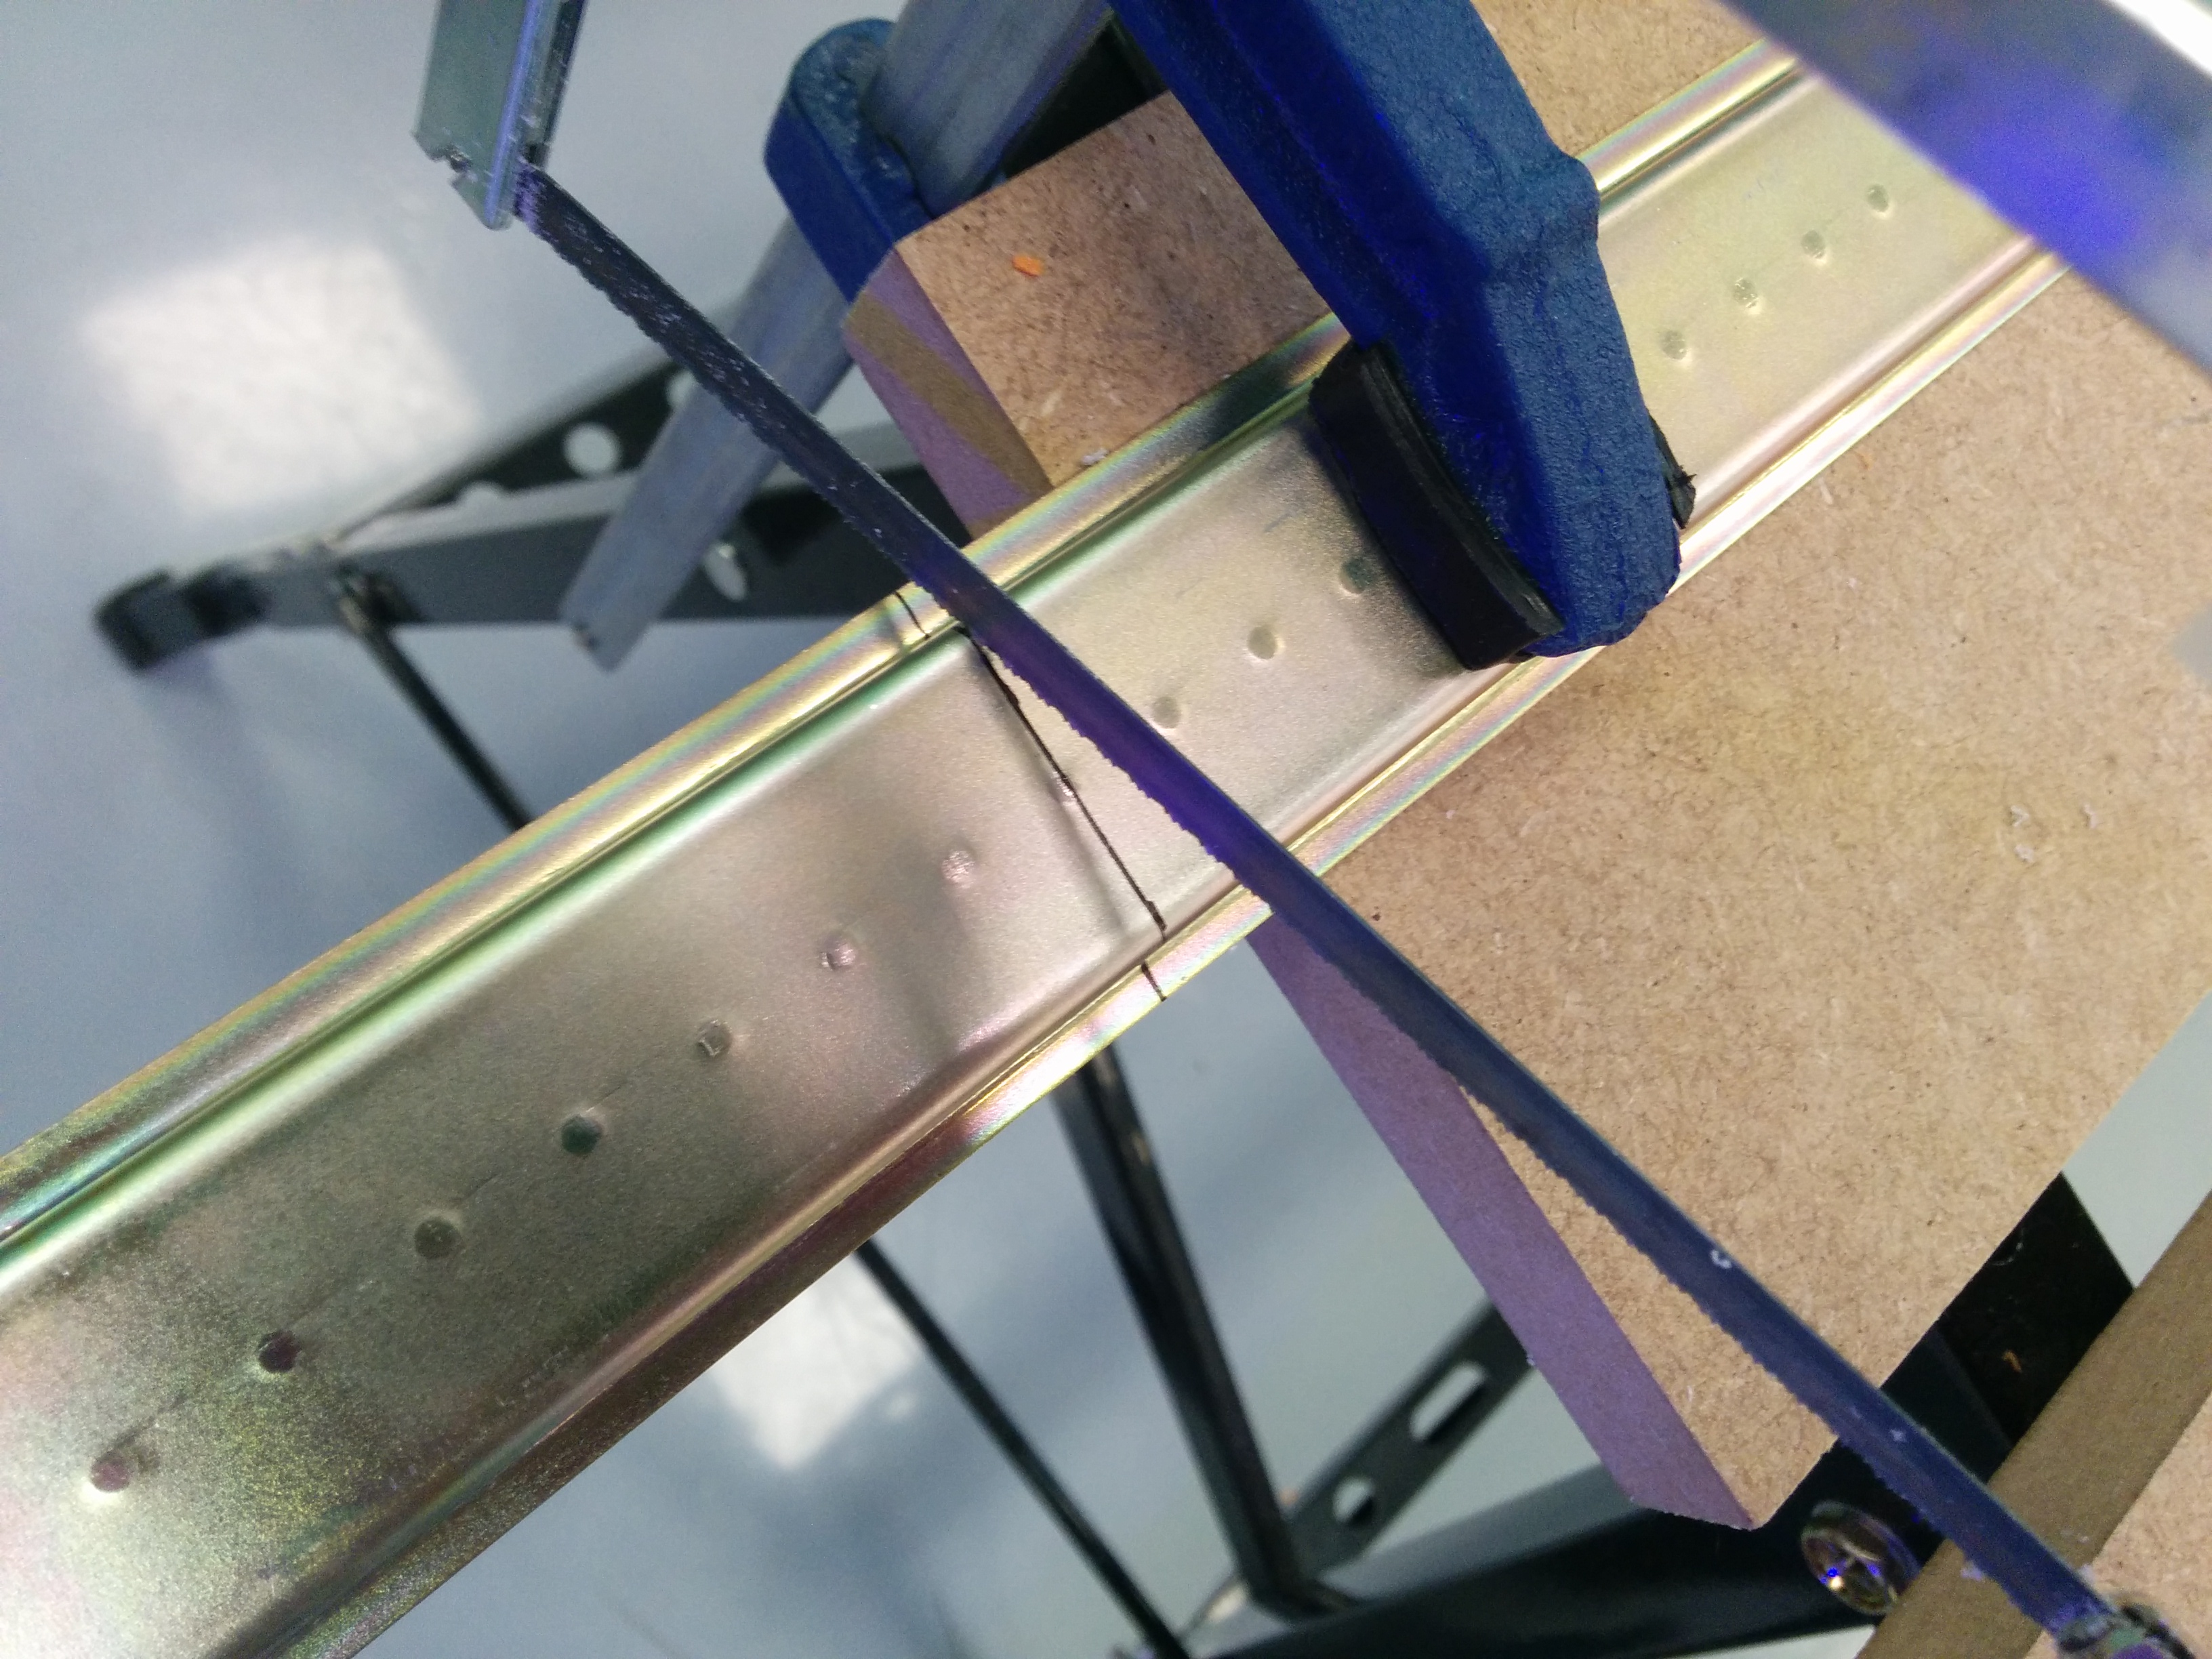
\includegraphics[width=0.5\textwidth]{images/cuadro/IMG_20150311_164348.jpg}
            \caption{Cortamos la guía y canaleta según las necesidades.}
            \label{fig:cuad_montaje2}
    \end{figure}
    \begin{figure}[H]
            \centering
            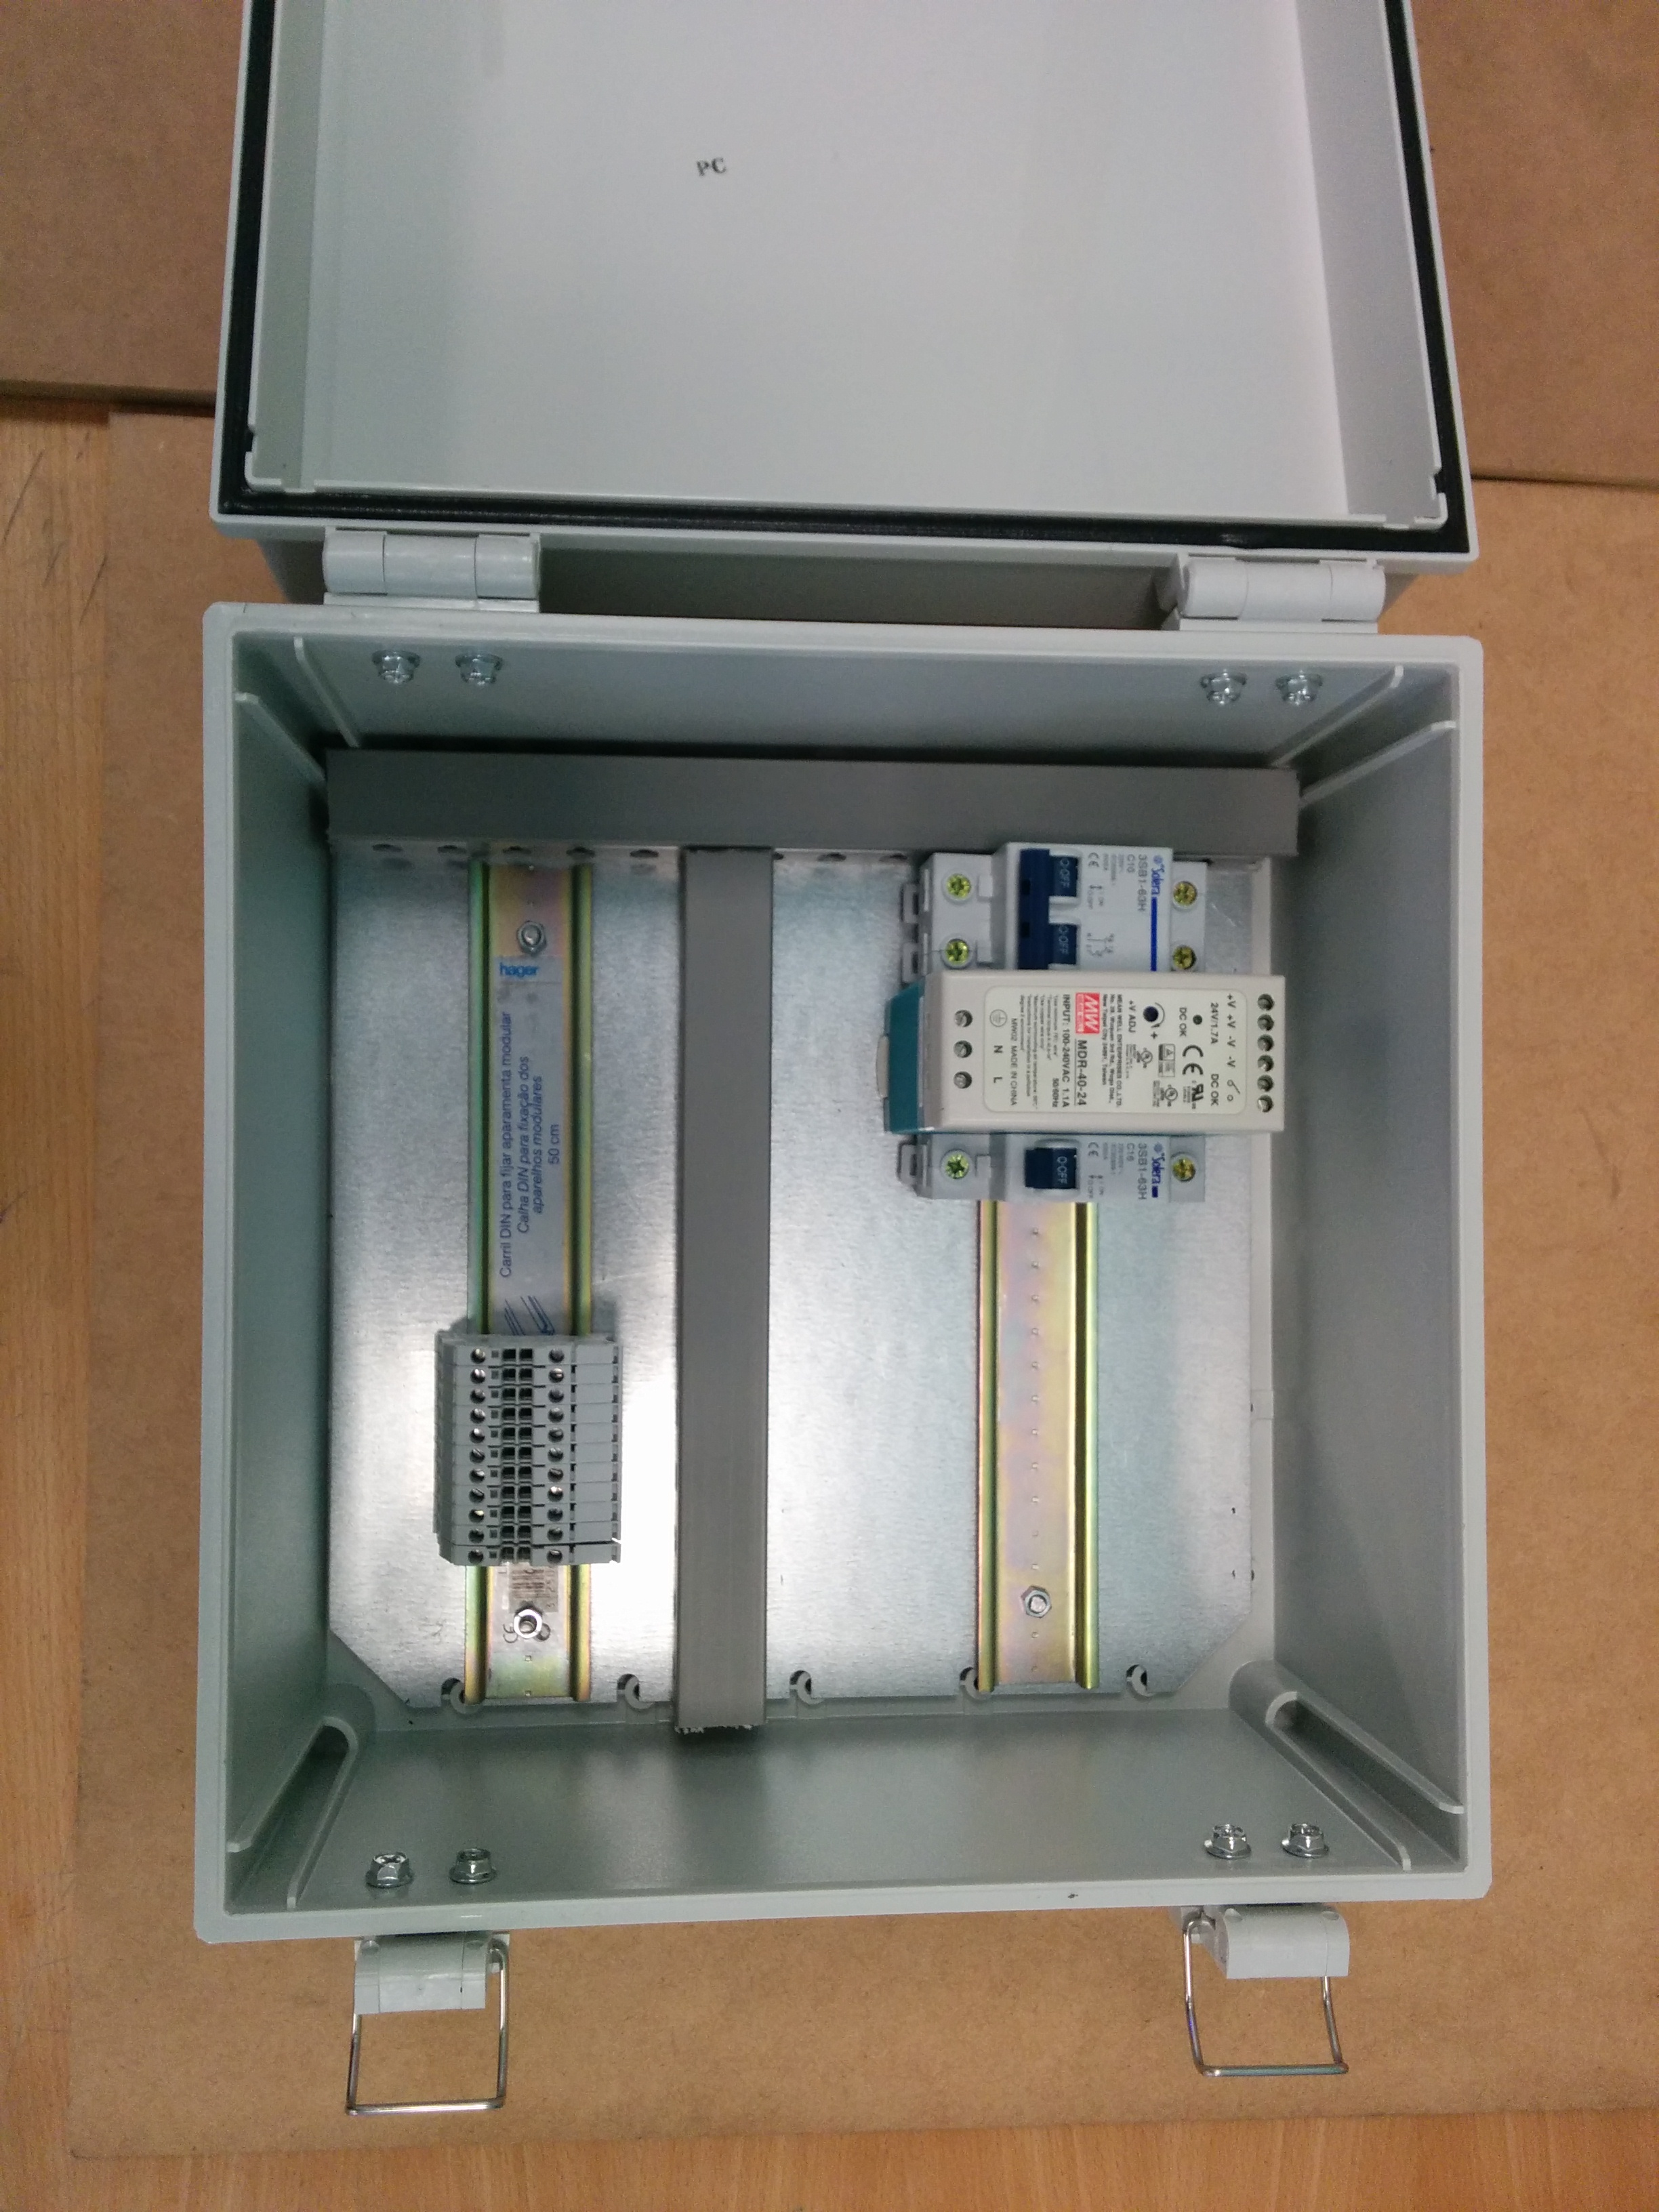
\includegraphics[width=0.5\textwidth]{images/cuadro/IMG_20150313_143943.jpg}
            \caption{Comprobamos que entra dentro del armario.}
            \label{fig:cuad_montaje3}
    \end{figure}
    \begin{figure}[H]
            \centering
            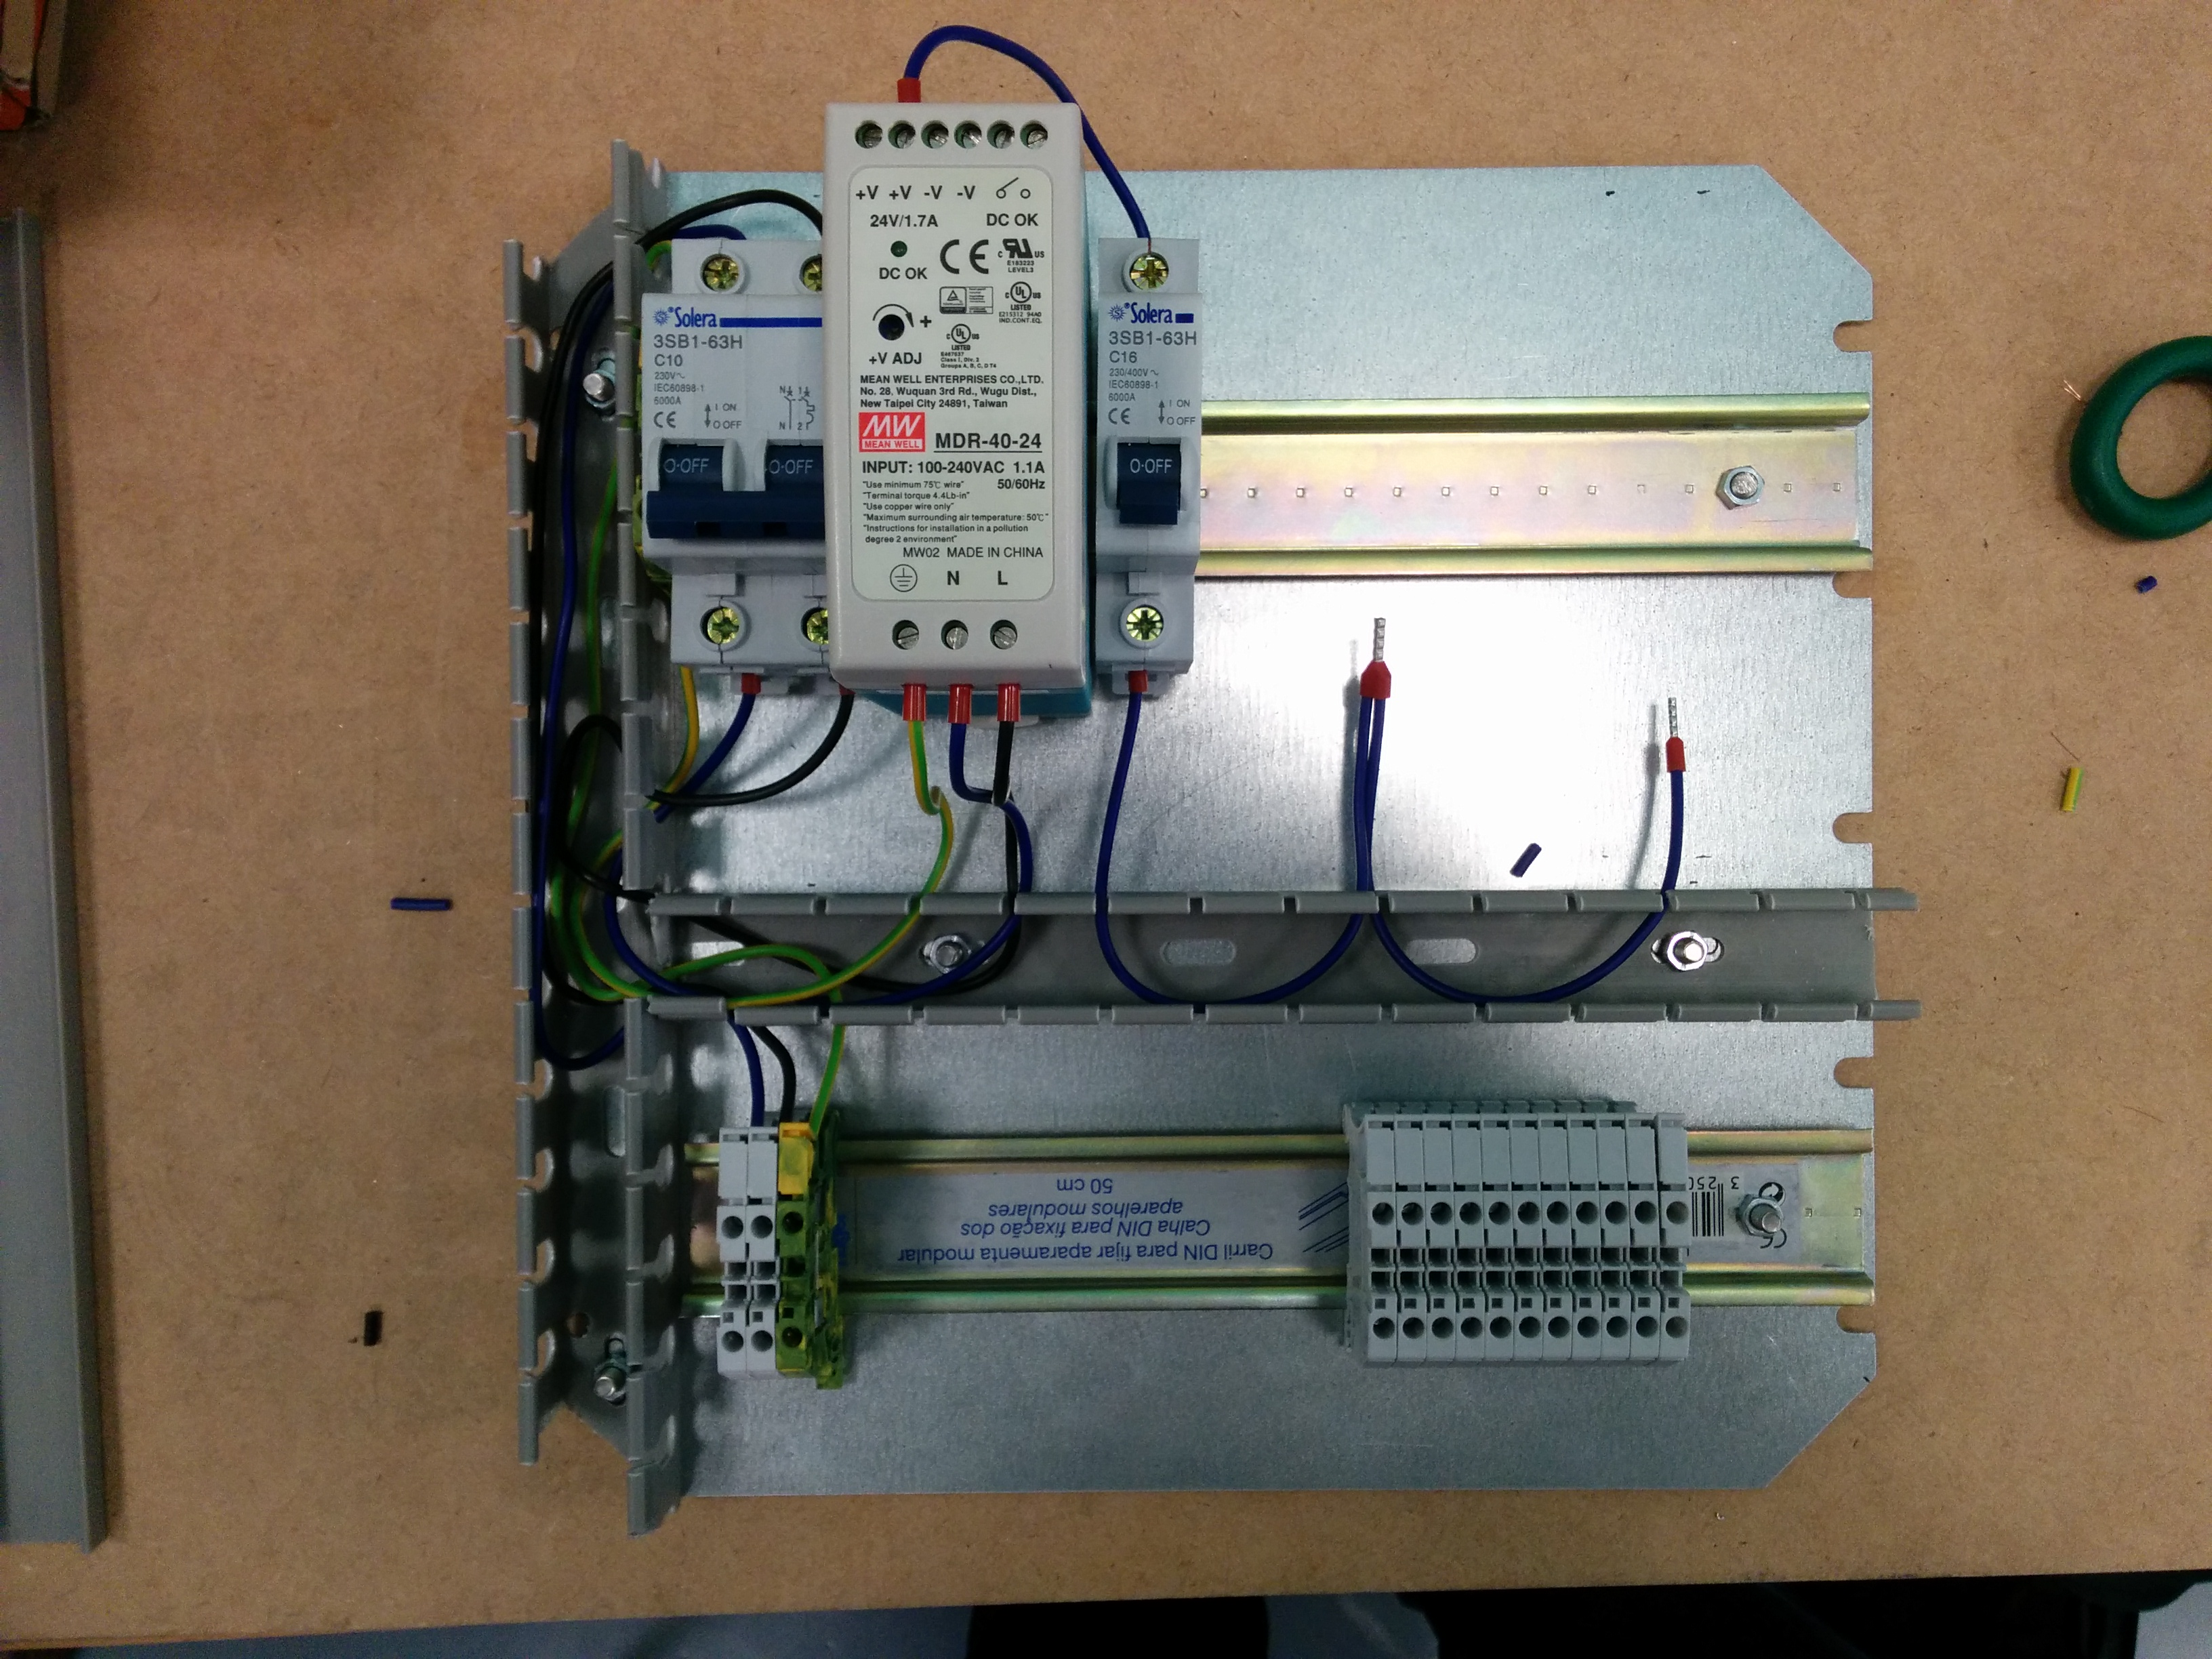
\includegraphics[width=0.5\textwidth]{images/cuadro/IMG_20150313_182301.jpg}
            \caption{Cableamos los dispositivos entre sí.}
            \label{fig:cuad_montaje4}
    \end{figure}
       \begin{figure}[H]
            \centering
            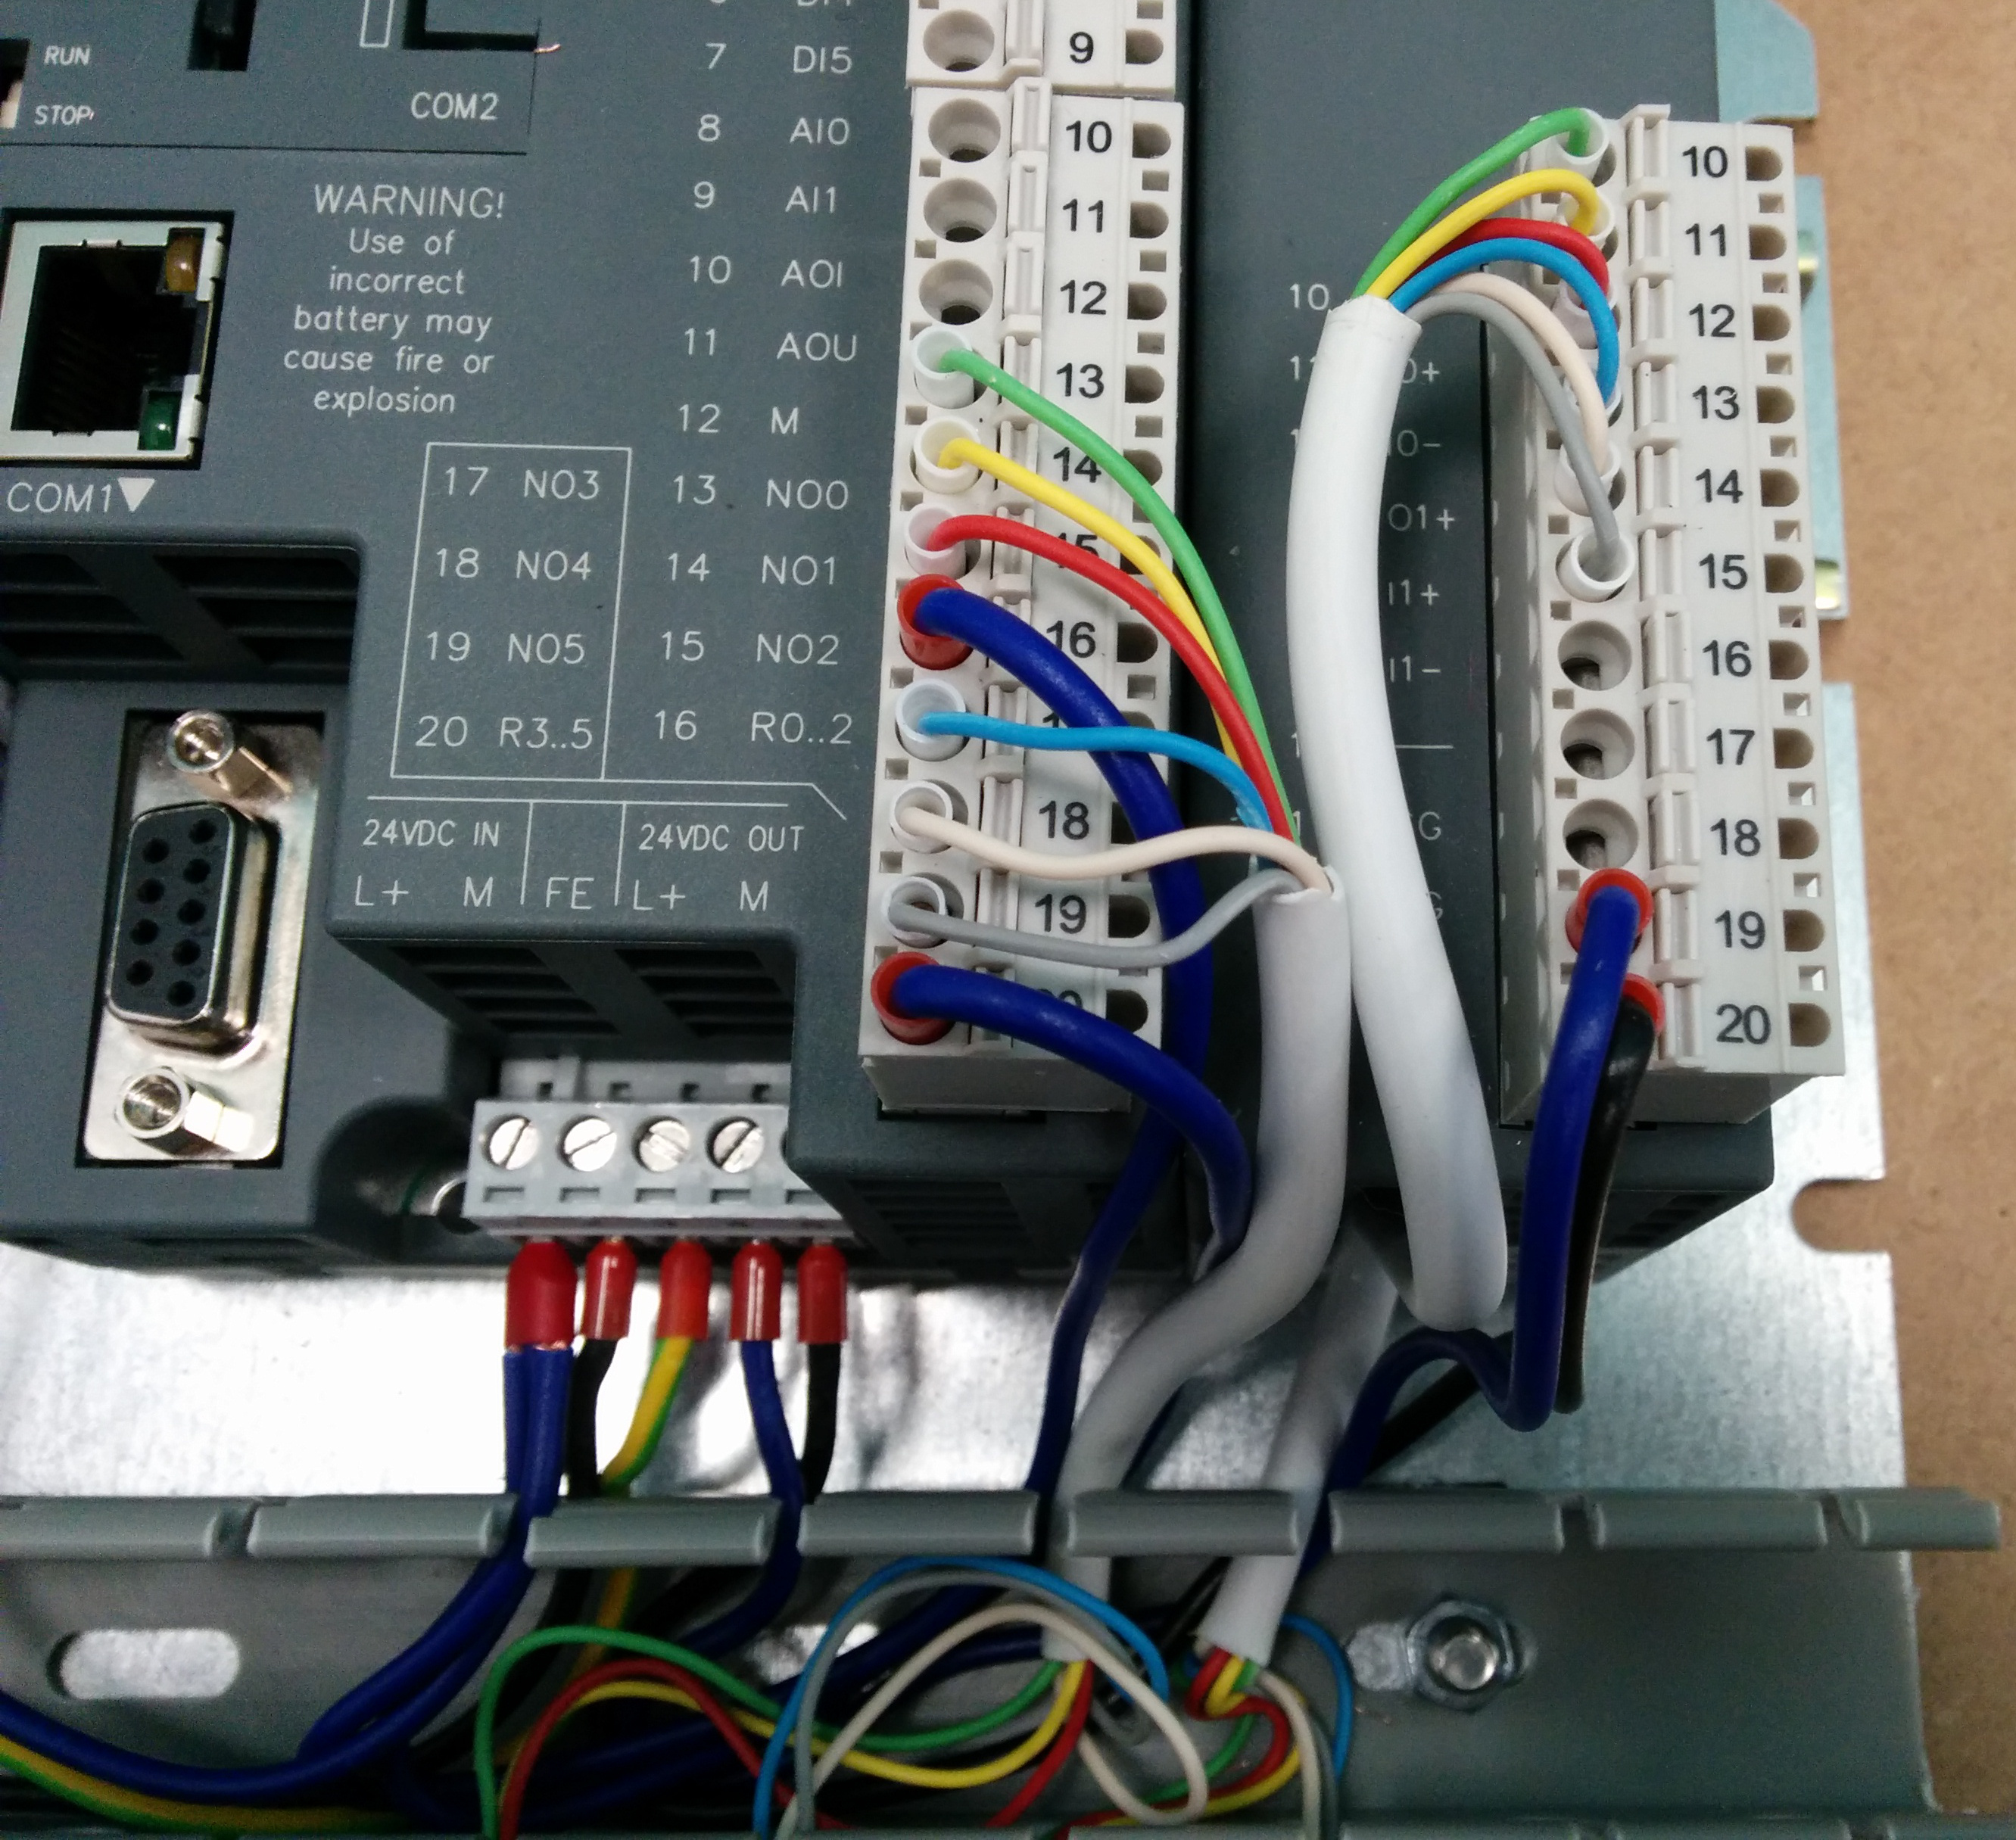
\includegraphics[width=0.5\textwidth]{images/cuadro/IMG_20150331_113600.jpg}
            \caption{Cableamos las entradas-salidas del PLC.}
            \label{fig:cuad_montaje5}
    \end{figure}
    \begin{figure}[H]
            \centering
            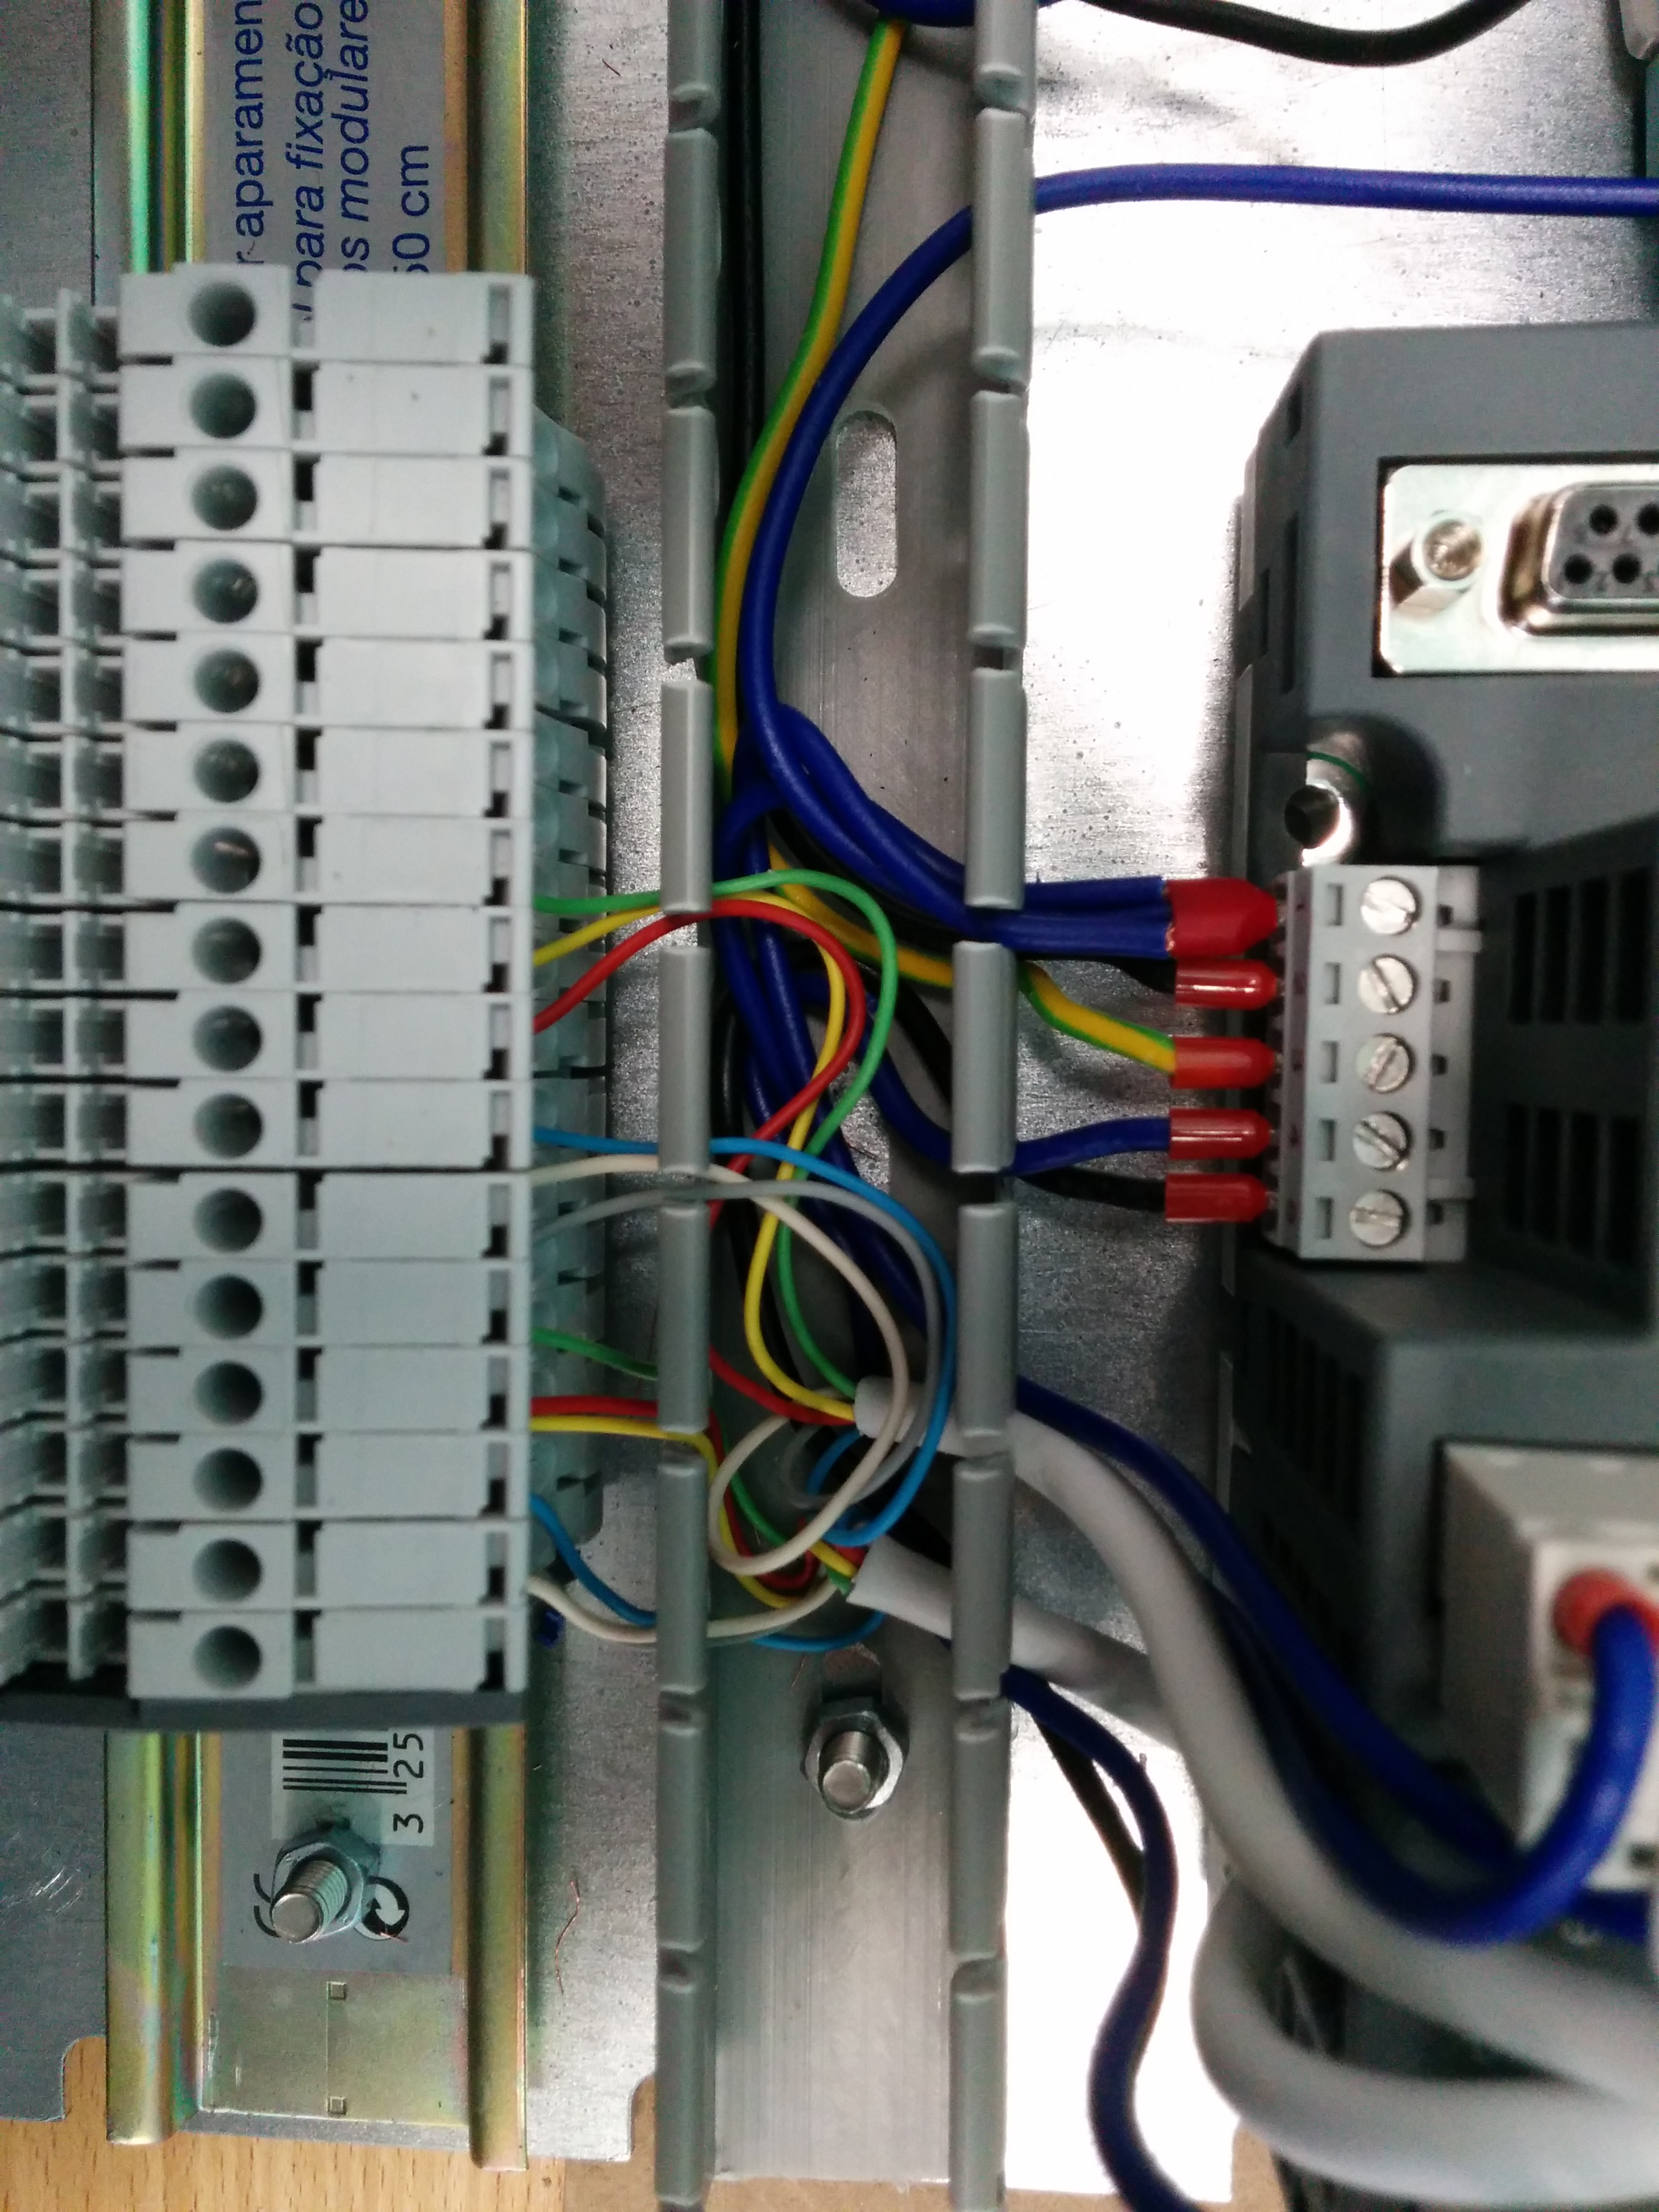
\includegraphics[width=0.5\textwidth]{images/cuadro/IMG_20150331_113607.jpg}
            \caption{Regletero con acceso a los pines del PLC.}
            \label{fig:cuad_montaje6}
    \end{figure}
    \begin{figure}[H]
            \centering
            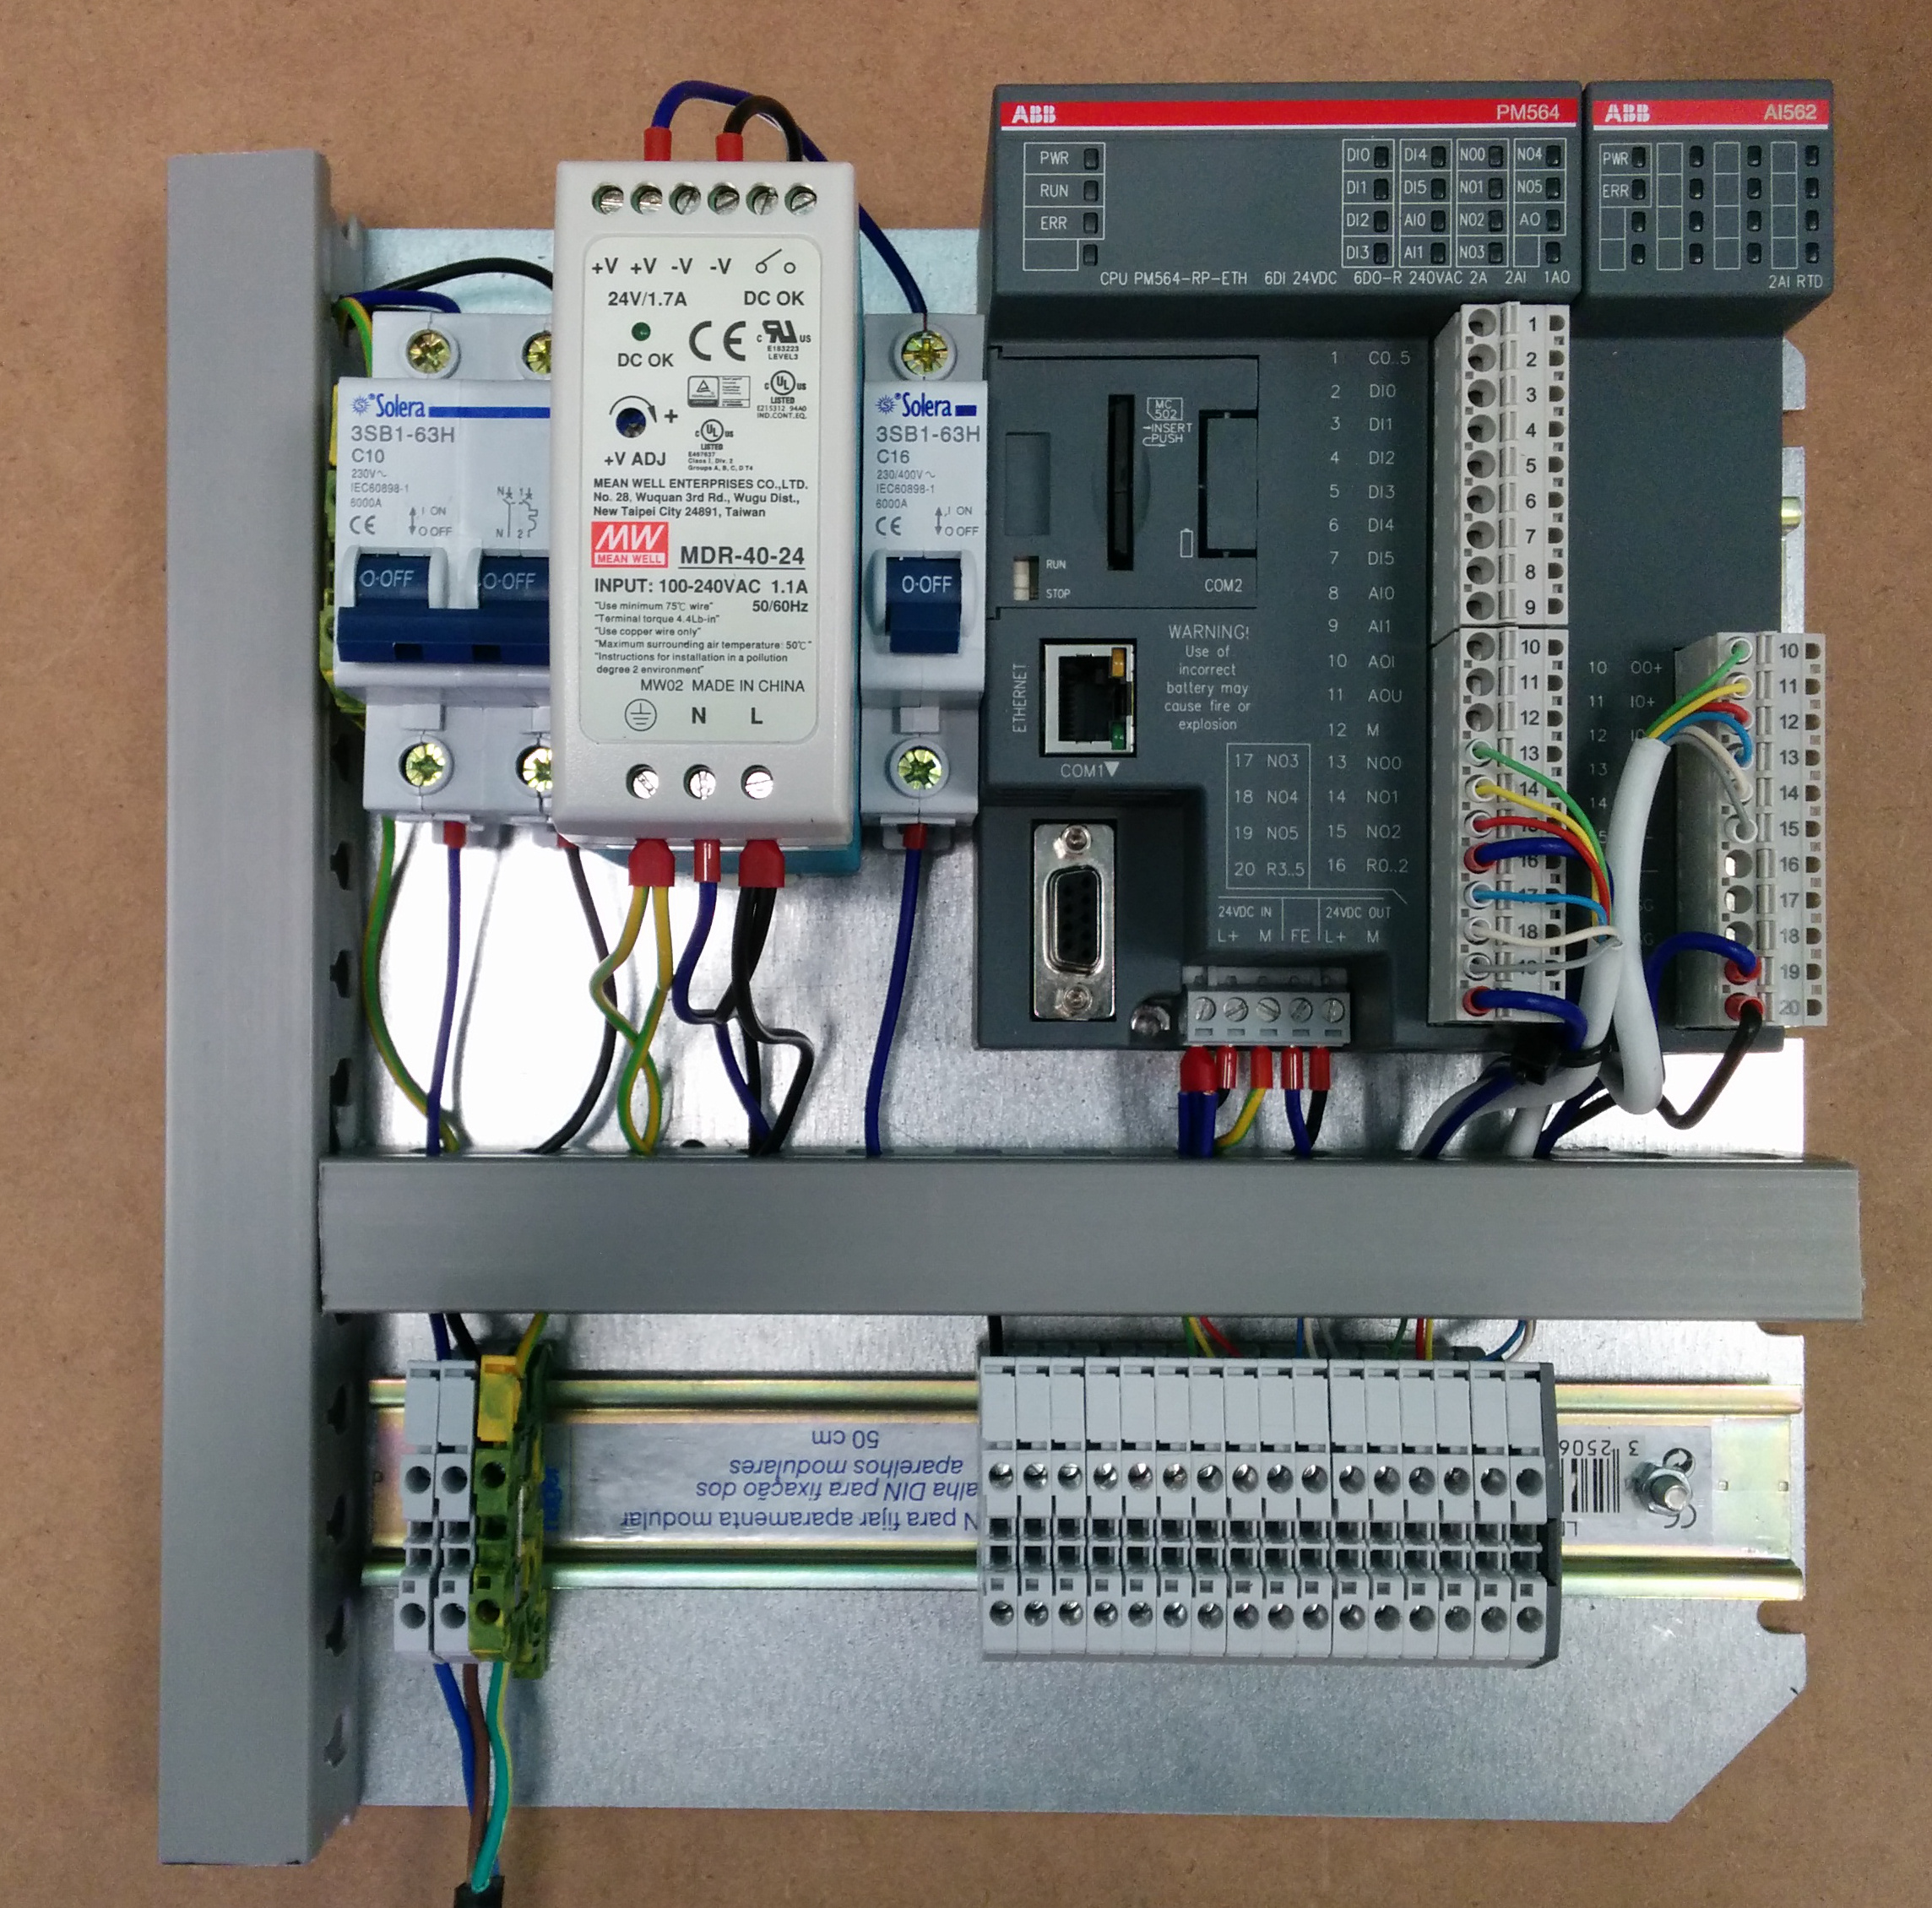
\includegraphics[width=0.5\textwidth]{images/cuadro/IMG_20150331_114950.jpg}
            \caption{Cuadro terminado.}
            \label{fig:cuad_montaje7}
    \end{figure}

Hasta el momento, hemos conseguido:

